% Generated by Sphinx.
\def\sphinxdocclass{report}
\documentclass[a4paper,12pt,spanish]{sphinxmanual}
\usepackage[utf8]{inputenc}
\DeclareUnicodeCharacter{00A0}{\nobreakspace}
\usepackage{cmap}
\usepackage[T1]{fontenc}
\usepackage{babel}
\usepackage{times}
\usepackage[Sonny]{fncychap}
\usepackage{longtable}
\usepackage{sphinx}
\usepackage{multirow}


\title{Programación de Servicios y Procesos}
\date{2014-2015}
\release{1.0}
\author{Oscar Gomez}
\newcommand{\sphinxlogo}{}
\renewcommand{\releasename}{Publicación}
\makeindex

\makeatletter
\def\PYG@reset{\let\PYG@it=\relax \let\PYG@bf=\relax%
    \let\PYG@ul=\relax \let\PYG@tc=\relax%
    \let\PYG@bc=\relax \let\PYG@ff=\relax}
\def\PYG@tok#1{\csname PYG@tok@#1\endcsname}
\def\PYG@toks#1+{\ifx\relax#1\empty\else%
    \PYG@tok{#1}\expandafter\PYG@toks\fi}
\def\PYG@do#1{\PYG@bc{\PYG@tc{\PYG@ul{%
    \PYG@it{\PYG@bf{\PYG@ff{#1}}}}}}}
\def\PYG#1#2{\PYG@reset\PYG@toks#1+\relax+\PYG@do{#2}}

\expandafter\def\csname PYG@tok@nv\endcsname{\def\PYG@tc##1{\textcolor[rgb]{0.73,0.38,0.84}{##1}}}
\expandafter\def\csname PYG@tok@sd\endcsname{\let\PYG@it=\textit\def\PYG@tc##1{\textcolor[rgb]{0.25,0.44,0.63}{##1}}}
\expandafter\def\csname PYG@tok@ss\endcsname{\def\PYG@tc##1{\textcolor[rgb]{0.32,0.47,0.09}{##1}}}
\expandafter\def\csname PYG@tok@s1\endcsname{\def\PYG@tc##1{\textcolor[rgb]{0.25,0.44,0.63}{##1}}}
\expandafter\def\csname PYG@tok@gp\endcsname{\let\PYG@bf=\textbf\def\PYG@tc##1{\textcolor[rgb]{0.78,0.36,0.04}{##1}}}
\expandafter\def\csname PYG@tok@vc\endcsname{\def\PYG@tc##1{\textcolor[rgb]{0.73,0.38,0.84}{##1}}}
\expandafter\def\csname PYG@tok@ni\endcsname{\let\PYG@bf=\textbf\def\PYG@tc##1{\textcolor[rgb]{0.84,0.33,0.22}{##1}}}
\expandafter\def\csname PYG@tok@no\endcsname{\def\PYG@tc##1{\textcolor[rgb]{0.38,0.68,0.84}{##1}}}
\expandafter\def\csname PYG@tok@vg\endcsname{\def\PYG@tc##1{\textcolor[rgb]{0.73,0.38,0.84}{##1}}}
\expandafter\def\csname PYG@tok@cs\endcsname{\def\PYG@tc##1{\textcolor[rgb]{0.25,0.50,0.56}{##1}}\def\PYG@bc##1{\setlength{\fboxsep}{0pt}\colorbox[rgb]{1.00,0.94,0.94}{\strut ##1}}}
\expandafter\def\csname PYG@tok@o\endcsname{\def\PYG@tc##1{\textcolor[rgb]{0.40,0.40,0.40}{##1}}}
\expandafter\def\csname PYG@tok@gu\endcsname{\let\PYG@bf=\textbf\def\PYG@tc##1{\textcolor[rgb]{0.50,0.00,0.50}{##1}}}
\expandafter\def\csname PYG@tok@ge\endcsname{\let\PYG@it=\textit}
\expandafter\def\csname PYG@tok@nd\endcsname{\let\PYG@bf=\textbf\def\PYG@tc##1{\textcolor[rgb]{0.33,0.33,0.33}{##1}}}
\expandafter\def\csname PYG@tok@c\endcsname{\let\PYG@it=\textit\def\PYG@tc##1{\textcolor[rgb]{0.25,0.50,0.56}{##1}}}
\expandafter\def\csname PYG@tok@err\endcsname{\def\PYG@bc##1{\setlength{\fboxsep}{0pt}\fcolorbox[rgb]{1.00,0.00,0.00}{1,1,1}{\strut ##1}}}
\expandafter\def\csname PYG@tok@bp\endcsname{\def\PYG@tc##1{\textcolor[rgb]{0.00,0.44,0.13}{##1}}}
\expandafter\def\csname PYG@tok@gs\endcsname{\let\PYG@bf=\textbf}
\expandafter\def\csname PYG@tok@kp\endcsname{\def\PYG@tc##1{\textcolor[rgb]{0.00,0.44,0.13}{##1}}}
\expandafter\def\csname PYG@tok@kt\endcsname{\def\PYG@tc##1{\textcolor[rgb]{0.56,0.13,0.00}{##1}}}
\expandafter\def\csname PYG@tok@vi\endcsname{\def\PYG@tc##1{\textcolor[rgb]{0.73,0.38,0.84}{##1}}}
\expandafter\def\csname PYG@tok@c1\endcsname{\let\PYG@it=\textit\def\PYG@tc##1{\textcolor[rgb]{0.25,0.50,0.56}{##1}}}
\expandafter\def\csname PYG@tok@si\endcsname{\let\PYG@it=\textit\def\PYG@tc##1{\textcolor[rgb]{0.44,0.63,0.82}{##1}}}
\expandafter\def\csname PYG@tok@cp\endcsname{\def\PYG@tc##1{\textcolor[rgb]{0.00,0.44,0.13}{##1}}}
\expandafter\def\csname PYG@tok@ne\endcsname{\def\PYG@tc##1{\textcolor[rgb]{0.00,0.44,0.13}{##1}}}
\expandafter\def\csname PYG@tok@k\endcsname{\let\PYG@bf=\textbf\def\PYG@tc##1{\textcolor[rgb]{0.00,0.44,0.13}{##1}}}
\expandafter\def\csname PYG@tok@sr\endcsname{\def\PYG@tc##1{\textcolor[rgb]{0.14,0.33,0.53}{##1}}}
\expandafter\def\csname PYG@tok@ow\endcsname{\let\PYG@bf=\textbf\def\PYG@tc##1{\textcolor[rgb]{0.00,0.44,0.13}{##1}}}
\expandafter\def\csname PYG@tok@mf\endcsname{\def\PYG@tc##1{\textcolor[rgb]{0.13,0.50,0.31}{##1}}}
\expandafter\def\csname PYG@tok@mo\endcsname{\def\PYG@tc##1{\textcolor[rgb]{0.13,0.50,0.31}{##1}}}
\expandafter\def\csname PYG@tok@gt\endcsname{\def\PYG@tc##1{\textcolor[rgb]{0.00,0.27,0.87}{##1}}}
\expandafter\def\csname PYG@tok@mi\endcsname{\def\PYG@tc##1{\textcolor[rgb]{0.13,0.50,0.31}{##1}}}
\expandafter\def\csname PYG@tok@mh\endcsname{\def\PYG@tc##1{\textcolor[rgb]{0.13,0.50,0.31}{##1}}}
\expandafter\def\csname PYG@tok@nl\endcsname{\let\PYG@bf=\textbf\def\PYG@tc##1{\textcolor[rgb]{0.00,0.13,0.44}{##1}}}
\expandafter\def\csname PYG@tok@w\endcsname{\def\PYG@tc##1{\textcolor[rgb]{0.73,0.73,0.73}{##1}}}
\expandafter\def\csname PYG@tok@nf\endcsname{\def\PYG@tc##1{\textcolor[rgb]{0.02,0.16,0.49}{##1}}}
\expandafter\def\csname PYG@tok@gd\endcsname{\def\PYG@tc##1{\textcolor[rgb]{0.63,0.00,0.00}{##1}}}
\expandafter\def\csname PYG@tok@m\endcsname{\def\PYG@tc##1{\textcolor[rgb]{0.13,0.50,0.31}{##1}}}
\expandafter\def\csname PYG@tok@kc\endcsname{\let\PYG@bf=\textbf\def\PYG@tc##1{\textcolor[rgb]{0.00,0.44,0.13}{##1}}}
\expandafter\def\csname PYG@tok@kd\endcsname{\let\PYG@bf=\textbf\def\PYG@tc##1{\textcolor[rgb]{0.00,0.44,0.13}{##1}}}
\expandafter\def\csname PYG@tok@kn\endcsname{\let\PYG@bf=\textbf\def\PYG@tc##1{\textcolor[rgb]{0.00,0.44,0.13}{##1}}}
\expandafter\def\csname PYG@tok@gh\endcsname{\let\PYG@bf=\textbf\def\PYG@tc##1{\textcolor[rgb]{0.00,0.00,0.50}{##1}}}
\expandafter\def\csname PYG@tok@cm\endcsname{\let\PYG@it=\textit\def\PYG@tc##1{\textcolor[rgb]{0.25,0.50,0.56}{##1}}}
\expandafter\def\csname PYG@tok@sc\endcsname{\def\PYG@tc##1{\textcolor[rgb]{0.25,0.44,0.63}{##1}}}
\expandafter\def\csname PYG@tok@gr\endcsname{\def\PYG@tc##1{\textcolor[rgb]{1.00,0.00,0.00}{##1}}}
\expandafter\def\csname PYG@tok@kr\endcsname{\let\PYG@bf=\textbf\def\PYG@tc##1{\textcolor[rgb]{0.00,0.44,0.13}{##1}}}
\expandafter\def\csname PYG@tok@na\endcsname{\def\PYG@tc##1{\textcolor[rgb]{0.25,0.44,0.63}{##1}}}
\expandafter\def\csname PYG@tok@sb\endcsname{\def\PYG@tc##1{\textcolor[rgb]{0.25,0.44,0.63}{##1}}}
\expandafter\def\csname PYG@tok@il\endcsname{\def\PYG@tc##1{\textcolor[rgb]{0.13,0.50,0.31}{##1}}}
\expandafter\def\csname PYG@tok@nn\endcsname{\let\PYG@bf=\textbf\def\PYG@tc##1{\textcolor[rgb]{0.05,0.52,0.71}{##1}}}
\expandafter\def\csname PYG@tok@nt\endcsname{\let\PYG@bf=\textbf\def\PYG@tc##1{\textcolor[rgb]{0.02,0.16,0.45}{##1}}}
\expandafter\def\csname PYG@tok@go\endcsname{\def\PYG@tc##1{\textcolor[rgb]{0.20,0.20,0.20}{##1}}}
\expandafter\def\csname PYG@tok@se\endcsname{\let\PYG@bf=\textbf\def\PYG@tc##1{\textcolor[rgb]{0.25,0.44,0.63}{##1}}}
\expandafter\def\csname PYG@tok@sh\endcsname{\def\PYG@tc##1{\textcolor[rgb]{0.25,0.44,0.63}{##1}}}
\expandafter\def\csname PYG@tok@s2\endcsname{\def\PYG@tc##1{\textcolor[rgb]{0.25,0.44,0.63}{##1}}}
\expandafter\def\csname PYG@tok@gi\endcsname{\def\PYG@tc##1{\textcolor[rgb]{0.00,0.63,0.00}{##1}}}
\expandafter\def\csname PYG@tok@sx\endcsname{\def\PYG@tc##1{\textcolor[rgb]{0.78,0.36,0.04}{##1}}}
\expandafter\def\csname PYG@tok@nc\endcsname{\let\PYG@bf=\textbf\def\PYG@tc##1{\textcolor[rgb]{0.05,0.52,0.71}{##1}}}
\expandafter\def\csname PYG@tok@s\endcsname{\def\PYG@tc##1{\textcolor[rgb]{0.25,0.44,0.63}{##1}}}
\expandafter\def\csname PYG@tok@nb\endcsname{\def\PYG@tc##1{\textcolor[rgb]{0.00,0.44,0.13}{##1}}}

\def\PYGZbs{\char`\\}
\def\PYGZus{\char`\_}
\def\PYGZob{\char`\{}
\def\PYGZcb{\char`\}}
\def\PYGZca{\char`\^}
\def\PYGZam{\char`\&}
\def\PYGZlt{\char`\<}
\def\PYGZgt{\char`\>}
\def\PYGZsh{\char`\#}
\def\PYGZpc{\char`\%}
\def\PYGZdl{\char`\$}
\def\PYGZhy{\char`\-}
\def\PYGZsq{\char`\'}
\def\PYGZdq{\char`\"}
\def\PYGZti{\char`\~}
% for compatibility with earlier versions
\def\PYGZat{@}
\def\PYGZlb{[}
\def\PYGZrb{]}
\makeatother

\renewcommand\PYGZsq{\textquotesingle}

\begin{document}
\shorthandoff{"}
\maketitle
\tableofcontents
\phantomsection\label{index::doc}



\chapter{Programación multiproceso}
\label{textos/tema1:programacion-de-servicios-y-procesos}\label{textos/tema1::doc}\label{textos/tema1:programacion-multiproceso}

\section{Ejecutables. Procesos. Servicios.}
\label{textos/tema1:ejecutables-procesos-servicios}

\subsection{Ejecutables}
\label{textos/tema1:ejecutables}
Un ejecutable es un archivo con la estructura necesaria para que el sistema operativo pueda poner en marcha el programa que hay dentro. En Windows, los ejecutables suelen ser archivos con la extension .EXE.

Sin embargo, Java genera ficheros .JAR o .CLASS. Estos ficheros \emph{no son ejecutables} sino que son archivos que el intérprete de JAVA (el archivo \code{java.exe}) leerá y ejecutará.

El intérprete toma el programa y lo traduce a instrucciones del microprocesador en el que estemos, que puede ser x86 o un x64 o lo que sea. Ese proceso se hace ``al instante'' o JIT (Just-In-Time).

Un EXE puede que no contenga las instrucciones de los microprocesadores más modernos. Como todos son compatibles no es un gran problema, sin embargo, puede que no aprovechemos al 100\% la capacidad de nuestro micro.


\subsection{Procesos}
\label{textos/tema1:procesos}
Es un archivo que está en ejecución y bajo el control del sistema operativo. Un proceso puede atravesar diversas etapas en su ``ciclo de vida''. Los estados en los que puede estar son:
\begin{itemize}
\item {} 
En ejecución: está dentro del microprocesador.

\item {} 
Pausado/detenido/en espera: el proceso tiene que seguir en ejecución pero en ese momento el S.O tomó la decisión de dejar paso a otro.

\item {} 
Interrumpido: el proceso tiene que seguir en ejecución pero \emph{el usuario} ha decidido interrumpir la ejecución.

\item {} 
Existen otros estados pero ya son muy dependientes del sistema operativo concreto.

\end{itemize}


\subsection{Servicios}
\label{textos/tema1:servicios}
Un servicio es un proceso que no muestra ninguna ventana ni gráfico en pantalla porque no está pensado para que el usuario lo maneje directamente.

Habitualmente, un servicio es un programa que atiende a otro programa.


\section{Hilos.}
\label{textos/tema1:hilos}
Un hilo es un concepto más avanzado que un proceso: al hablar de procesos cada uno tiene su propio espacio en memoria. Si abrimos 20 procesos cada uno de ellos consume 20x de memoria RAM. Un hilo es un proceso mucho más ligero, en el que el código y los datos se comparten de una forma distinta.

Un proceso no tiene acceso a los datos de otro procesos. Sin embargo un hilo sí accede a los datos de otro hilo. Esto complicará algunas cuestiones a la hora de programar.


\section{Programación concurrente.}
\label{textos/tema1:programacion-concurrente}
La programación concurrente es la parte de la programación que se ocupa de crear programas que pueden tener varios procesos/hilos que colaboran para ejecutar un trabajo y aprovechar al máximo el rendimiento de sistemas multinúcleo.


\section{Programación paralela y distribuida.}
\label{textos/tema1:programacion-paralela-y-distribuida}
Dentro de la programación concurrente tenemos la paralela y la distribuida:
\begin{itemize}
\item {} 
En general se denomina ``programación paralela'' a la creación de software que se ejecuta siempre en un solo ordenador (con varios núcleos o no)

\item {} 
Se denomina ``programación distribuida'' a la creación de software que se ejecuta en ordenadores distintos y que se comunican a través de una red.

\end{itemize}


\section{Creación de procesos.}
\label{textos/tema1:creacion-de-procesos}
En Java es posible crear procesos utilizando algunas clases que el entorno ofrece para esta tarea. En este tema, veremos en profundidad la clase ProcessBuilder.

El ejemplo siguiente muestra como lanzar un proceso de Acrobat Reader:

\begin{Verbatim}[commandchars=\\\{\}]
\PYG{k+kd}{public} \PYG{k+kd}{class} \PYG{n+nc}{LanzadorProcesos} \PYG{o}{\PYGZob{}}
        \PYG{k+kd}{public} \PYG{k+kt}{void} \PYG{n+nf}{ejecutar}\PYG{o}{(}\PYG{n}{String} \PYG{n}{ruta}\PYG{o}{)}\PYG{o}{\PYGZob{}}

                \PYG{n}{ProcessBuilder} \PYG{n}{pb}\PYG{o}{;}
                \PYG{k}{try} \PYG{o}{\PYGZob{}}
                        \PYG{n}{pb} \PYG{o}{=} \PYG{k}{new} \PYG{n}{ProcessBuilder}\PYG{o}{(}\PYG{n}{ruta}\PYG{o}{)}\PYG{o}{;}
                        \PYG{n}{pb}\PYG{o}{.}\PYG{n+na}{start}\PYG{o}{(}\PYG{o}{)}\PYG{o}{;}
                \PYG{o}{\PYGZcb{}} \PYG{k}{catch} \PYG{o}{(}\PYG{n}{Exception} \PYG{n}{e}\PYG{o}{)} \PYG{o}{\PYGZob{}}
                        \PYG{c+c1}{// TODO Auto\PYGZhy{}generated catch block}
                        \PYG{n}{e}\PYG{o}{.}\PYG{n+na}{printStackTrace}\PYG{o}{(}\PYG{o}{)}\PYG{o}{;}
                \PYG{o}{\PYGZcb{}}

        \PYG{o}{\PYGZcb{}}
        \PYG{c+cm}{/**}
\PYG{c+cm}{         * @param args}
\PYG{c+cm}{         */}
        \PYG{k+kd}{public} \PYG{k+kd}{static} \PYG{k+kt}{void} \PYG{n+nf}{main}\PYG{o}{(}\PYG{n}{String}\PYG{o}{[}\PYG{o}{]} \PYG{n}{args}\PYG{o}{)} \PYG{o}{\PYGZob{}}
                \PYG{n}{String} \PYG{n}{ruta}\PYG{o}{=}
                        \PYG{l+s}{\PYGZdq{}C:\PYGZbs{}\PYGZbs{}Program Files (x86)\PYGZbs{}\PYGZbs{}Adobe\PYGZbs{}\PYGZbs{}Reader 11.0\PYGZbs{}\PYGZbs{}Reader\PYGZbs{}\PYGZbs{}AcroRd32.exe\PYGZdq{}}\PYG{o}{;}
                \PYG{n}{LanzadorProcesos} \PYG{n}{lp}\PYG{o}{=}\PYG{k}{new} \PYG{n}{LanzadorProcesos}\PYG{o}{(}\PYG{o}{)}\PYG{o}{;}
                \PYG{n}{lp}\PYG{o}{.}\PYG{n+na}{ejecutar}\PYG{o}{(}\PYG{n}{ruta}\PYG{o}{)}\PYG{o}{;}
                \PYG{n}{System}\PYG{o}{.}\PYG{n+na}{out}\PYG{o}{.}\PYG{n+na}{println}\PYG{o}{(}\PYG{l+s}{\PYGZdq{}Finalizado\PYGZdq{}}\PYG{o}{)}\PYG{o}{;}
        \PYG{o}{\PYGZcb{}}

\PYG{o}{\PYGZcb{}}
\end{Verbatim}

Supongamos que necesitamos crear un programa que aproveche al máximo el número de CPUs para realizar alguna tarea intensiva. Supongamos que dicha tarea consiste en sumar números.

Enunciado: crear una clase Java que sea capaz de sumar todos los números comprendidos entre dos valores incluyendo ambos valores.

Para resolverlo crearemos una clase \code{Sumador} que tenga un método que acepte dos números \code{n1} y \code{n2} y que devuelva la suma de todo el intervalor.

Además, incluiremos un método \code{main} que ejecute la operación de suma tomando los números de la línea de comandos (es decir, se pasan como argumentos al main).

El código de dicha clase podría ser algo así:

\begin{Verbatim}[commandchars=\\\{\}]
\PYG{k+kn}{package} \PYG{n}{com}\PYG{o}{.}\PYG{n+na}{ies}\PYG{o}{;}

\PYG{k+kd}{public} \PYG{k+kd}{class} \PYG{n+nc}{Sumador} \PYG{o}{\PYGZob{}}
        \PYG{k+kd}{public} \PYG{k+kt}{int} \PYG{n+nf}{sumar}\PYG{o}{(}\PYG{k+kt}{int} \PYG{n}{n1}\PYG{o}{,} \PYG{k+kt}{int} \PYG{n}{n2}\PYG{o}{)}\PYG{o}{\PYGZob{}}
                \PYG{k+kt}{int} \PYG{n}{resultado}\PYG{o}{=}\PYG{l+m+mi}{0}\PYG{o}{;}
                \PYG{k}{for} \PYG{o}{(}\PYG{k+kt}{int} \PYG{n}{i}\PYG{o}{=}\PYG{n}{n1}\PYG{o}{;}\PYG{n}{i}\PYG{o}{\PYGZlt{}}\PYG{o}{=}\PYG{n}{n2}\PYG{o}{;}\PYG{n}{i}\PYG{o}{+}\PYG{o}{+}\PYG{o}{)}\PYG{o}{\PYGZob{}}
                        \PYG{n}{resultado}\PYG{o}{=}\PYG{n}{resultado}\PYG{o}{+}\PYG{n}{i}\PYG{o}{;}
                \PYG{o}{\PYGZcb{}}
                \PYG{k}{return} \PYG{n}{resultado}\PYG{o}{;}
        \PYG{o}{\PYGZcb{}}
        \PYG{k+kd}{public} \PYG{k+kd}{static} \PYG{k+kt}{void} \PYG{n+nf}{main}\PYG{o}{(}\PYG{n}{String}\PYG{o}{[}\PYG{o}{]} \PYG{n}{args}\PYG{o}{)}\PYG{o}{\PYGZob{}}
                \PYG{n}{Sumador} \PYG{n}{s}\PYG{o}{=}\PYG{k}{new} \PYG{n}{Sumador}\PYG{o}{(}\PYG{o}{)}\PYG{o}{;}
                \PYG{k+kt}{int} \PYG{n}{n1}\PYG{o}{=}\PYG{n}{Integer}\PYG{o}{.}\PYG{n+na}{parseInt}\PYG{o}{(}\PYG{n}{args}\PYG{o}{[}\PYG{l+m+mi}{0}\PYG{o}{]}\PYG{o}{)}\PYG{o}{;}
                \PYG{k+kt}{int} \PYG{n}{n2}\PYG{o}{=}\PYG{n}{Integer}\PYG{o}{.}\PYG{n+na}{parseInt}\PYG{o}{(}\PYG{n}{args}\PYG{o}{[}\PYG{l+m+mi}{1}\PYG{o}{]}\PYG{o}{)}\PYG{o}{;}
                \PYG{k+kt}{int} \PYG{n}{resultado}\PYG{o}{=}\PYG{n}{s}\PYG{o}{.}\PYG{n+na}{sumar}\PYG{o}{(}\PYG{n}{n1}\PYG{o}{,} \PYG{n}{n2}\PYG{o}{)}\PYG{o}{;}
                \PYG{n}{System}\PYG{o}{.}\PYG{n+na}{out}\PYG{o}{.}\PYG{n+na}{println}\PYG{o}{(}\PYG{n}{resultado}\PYG{o}{)}\PYG{o}{;}
        \PYG{o}{\PYGZcb{}}
\PYG{o}{\PYGZcb{}}
\end{Verbatim}

Para ejecutar este programa desde dentro de Eclipse es necesario indicar que deseamos enviar \emph{argumentos} al programa. Por ejemplo, si deseamos sumar los números del 2 al 10, deberemos ir a la venta ``Run configuration'' y en la pestaña ``Arguments'' indicar los argumentos (que en este caso son los dos números a indicar).
\begin{figure}[htbp]
\centering
\capstart

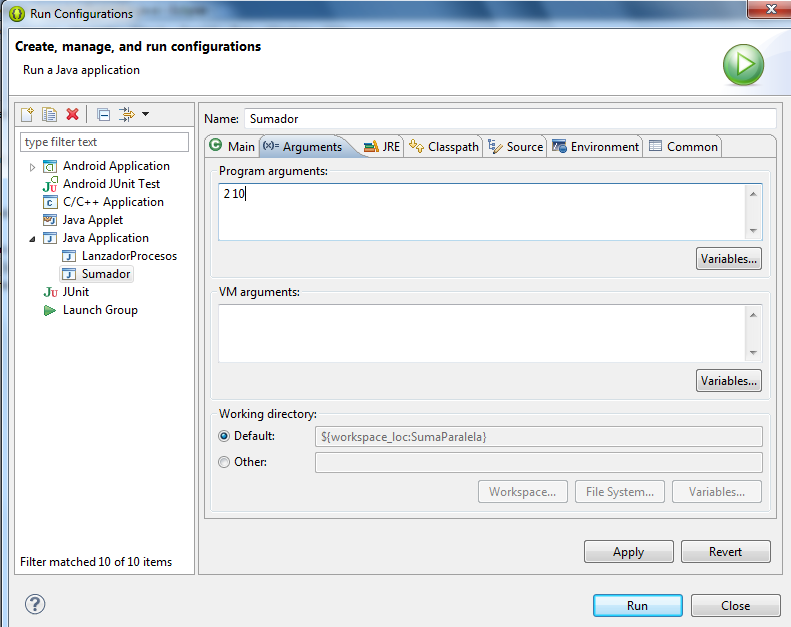
\includegraphics{configuraciones.png}
\caption{Modificando los argumentos del programa}\end{figure}

Una vez hecha la prueba de la clase sumador, le quitamos el main, y crearemos una clase que sea capaz de lanzar varios procesos. La clase \code{Sumador} se quedará así:

\begin{Verbatim}[commandchars=\\\{\}]
\PYG{k+kd}{public} \PYG{k+kd}{class} \PYG{n+nc}{Sumador} \PYG{o}{\PYGZob{}}
        \PYG{k+kd}{public} \PYG{k+kt}{int} \PYG{n+nf}{sumar}\PYG{o}{(}\PYG{k+kt}{int} \PYG{n}{n1}\PYG{o}{,} \PYG{k+kt}{int} \PYG{n}{n2}\PYG{o}{)}\PYG{o}{\PYGZob{}}
                \PYG{k+kt}{int} \PYG{n}{resultado}\PYG{o}{=}\PYG{l+m+mi}{0}\PYG{o}{;}
                \PYG{k}{for} \PYG{o}{(}\PYG{k+kt}{int} \PYG{n}{i}\PYG{o}{=}\PYG{n}{n1}\PYG{o}{;}\PYG{n}{i}\PYG{o}{\PYGZlt{}}\PYG{o}{=}\PYG{n}{n2}\PYG{o}{;}\PYG{n}{i}\PYG{o}{+}\PYG{o}{+}\PYG{o}{)}\PYG{o}{\PYGZob{}}
                        \PYG{n}{resultado}\PYG{o}{=}\PYG{n}{resultado}\PYG{o}{+}\PYG{n}{i}\PYG{o}{;}
                \PYG{o}{\PYGZcb{}}
                \PYG{k}{return} \PYG{n}{resultado}\PYG{o}{;}
        \PYG{o}{\PYGZcb{}}
\PYG{o}{\PYGZcb{}}
\end{Verbatim}

Y ahora tendremos una clase que lanza procesos de esta forma:

\begin{Verbatim}[commandchars=\\\{\}]
\PYG{k+kn}{package} \PYG{n}{com}\PYG{o}{.}\PYG{n+na}{ies}\PYG{o}{;}

\PYG{k+kd}{public} \PYG{k+kd}{class} \PYG{n+nc}{Lanzador} \PYG{o}{\PYGZob{}}
        \PYG{k+kd}{public} \PYG{k+kt}{void} \PYG{n+nf}{lanzarSumador}\PYG{o}{(}\PYG{n}{Integer} \PYG{n}{n1}\PYG{o}{,}
                        \PYG{n}{Integer} \PYG{n}{n2}\PYG{o}{)}\PYG{o}{\PYGZob{}}
                \PYG{n}{String} \PYG{n}{clase}\PYG{o}{=}\PYG{l+s}{\PYGZdq{}com.ies.Sumador\PYGZdq{}}\PYG{o}{;}
                \PYG{n}{ProcessBuilder} \PYG{n}{pb}\PYG{o}{;}
                \PYG{k}{try} \PYG{o}{\PYGZob{}}
                        \PYG{n}{pb} \PYG{o}{=} \PYG{k}{new} \PYG{n}{ProcessBuilder}\PYG{o}{(}
                                        \PYG{l+s}{\PYGZdq{}java\PYGZdq{}}\PYG{o}{,}\PYG{n}{clase}\PYG{o}{,}
                                        \PYG{n}{n1}\PYG{o}{.}\PYG{n+na}{toString}\PYG{o}{(}\PYG{o}{)}\PYG{o}{,}
                                        \PYG{n}{n2}\PYG{o}{.}\PYG{n+na}{toString}\PYG{o}{(}\PYG{o}{)}\PYG{o}{)}\PYG{o}{;}
                        \PYG{n}{pb}\PYG{o}{.}\PYG{n+na}{start}\PYG{o}{(}\PYG{o}{)}\PYG{o}{;}
                \PYG{o}{\PYGZcb{}} \PYG{k}{catch} \PYG{o}{(}\PYG{n}{Exception} \PYG{n}{e}\PYG{o}{)} \PYG{o}{\PYGZob{}}
                        \PYG{c+c1}{// TODO Auto\PYGZhy{}generated catch block}
                        \PYG{n}{e}\PYG{o}{.}\PYG{n+na}{printStackTrace}\PYG{o}{(}\PYG{o}{)}\PYG{o}{;}
                \PYG{o}{\PYGZcb{}}
        \PYG{o}{\PYGZcb{}}
        \PYG{k+kd}{public} \PYG{k+kd}{static} \PYG{k+kt}{void} \PYG{n+nf}{main}\PYG{o}{(}\PYG{n}{String}\PYG{o}{[}\PYG{o}{]} \PYG{n}{args}\PYG{o}{)}\PYG{o}{\PYGZob{}}
                \PYG{n}{Lanzador} \PYG{n}{l}\PYG{o}{=}\PYG{k}{new} \PYG{n}{Lanzador}\PYG{o}{(}\PYG{o}{)}\PYG{o}{;}
                \PYG{n}{l}\PYG{o}{.}\PYG{n+na}{lanzarSumador}\PYG{o}{(}\PYG{l+m+mi}{1}\PYG{o}{,} \PYG{l+m+mi}{51}\PYG{o}{)}\PYG{o}{;}
                \PYG{n}{l}\PYG{o}{.}\PYG{n+na}{lanzarSumador}\PYG{o}{(}\PYG{l+m+mi}{51}\PYG{o}{,} \PYG{l+m+mi}{100}\PYG{o}{)}\PYG{o}{;}
                \PYG{n}{System}\PYG{o}{.}\PYG{n+na}{out}\PYG{o}{.}\PYG{n+na}{println}\PYG{o}{(}\PYG{l+s}{\PYGZdq{}Ok\PYGZdq{}}\PYG{o}{)}\PYG{o}{;}
        \PYG{o}{\PYGZcb{}}
\PYG{o}{\PYGZcb{}}
\end{Verbatim}


\section{Comunicación entre procesos.}
\label{textos/tema1:comunicacion-entre-procesos}
Las operaciones multiproceso pueden implicar que sea necesario comunicar información entre muchos procesos, lo que obliga a la necesidad de utilizar mecanismos específicos de comunicación que ofrecerá Java o a diseñar alguno separado que evite los problemas que puedan aparecer.

En el ejemplo, el segundo proceso suele sobreescribir el resultado del primero, así que modificaremos el código del lanzador para que cada proceso use su propio fichero de resultados.

\begin{Verbatim}[commandchars=\\\{\}]
\PYG{k+kd}{public} \PYG{k+kd}{class} \PYG{n+nc}{Lanzador} \PYG{o}{\PYGZob{}}
        \PYG{k+kd}{public} \PYG{k+kt}{void} \PYG{n+nf}{lanzarSumador}\PYG{o}{(}\PYG{n}{Integer} \PYG{n}{n1}\PYG{o}{,}
                        \PYG{n}{Integer} \PYG{n}{n2}\PYG{o}{,} \PYG{n}{String} \PYG{n}{fichResultado}\PYG{o}{)}\PYG{o}{\PYGZob{}}
                \PYG{n}{String} \PYG{n}{clase}\PYG{o}{=}\PYG{l+s}{\PYGZdq{}com.ies.Sumador\PYGZdq{}}\PYG{o}{;}
                \PYG{n}{ProcessBuilder} \PYG{n}{pb}\PYG{o}{;}
                \PYG{k}{try} \PYG{o}{\PYGZob{}}
                        \PYG{n}{pb} \PYG{o}{=} \PYG{k}{new} \PYG{n}{ProcessBuilder}\PYG{o}{(}
                                        \PYG{l+s}{\PYGZdq{}java\PYGZdq{}}\PYG{o}{,}\PYG{n}{clase}\PYG{o}{,}
                                        \PYG{n}{n1}\PYG{o}{.}\PYG{n+na}{toString}\PYG{o}{(}\PYG{o}{)}\PYG{o}{,}
                                        \PYG{n}{n2}\PYG{o}{.}\PYG{n+na}{toString}\PYG{o}{(}\PYG{o}{)}\PYG{o}{)}\PYG{o}{;}

                        \PYG{n}{pb}\PYG{o}{.}\PYG{n+na}{redirectError}\PYG{o}{(}\PYG{k}{new} \PYG{n}{File}\PYG{o}{(}\PYG{l+s}{\PYGZdq{}errores.txt\PYGZdq{}}\PYG{o}{)}\PYG{o}{)}\PYG{o}{;}
                        \PYG{n}{pb}\PYG{o}{.}\PYG{n+na}{redirectOutput}\PYG{o}{(}\PYG{k}{new} \PYG{n}{File}\PYG{o}{(}\PYG{n}{fichResultado}\PYG{o}{)}\PYG{o}{)}\PYG{o}{;}
                        \PYG{n}{pb}\PYG{o}{.}\PYG{n+na}{start}\PYG{o}{(}\PYG{o}{)}\PYG{o}{;}
                \PYG{o}{\PYGZcb{}} \PYG{k}{catch} \PYG{o}{(}\PYG{n}{Exception} \PYG{n}{e}\PYG{o}{)} \PYG{o}{\PYGZob{}}
                        \PYG{c+c1}{// TODO Auto\PYGZhy{}generated catch block}
                        \PYG{n}{e}\PYG{o}{.}\PYG{n+na}{printStackTrace}\PYG{o}{(}\PYG{o}{)}\PYG{o}{;}
                \PYG{o}{\PYGZcb{}}
        \PYG{o}{\PYGZcb{}}
        \PYG{k+kd}{public} \PYG{k+kd}{static} \PYG{k+kt}{void} \PYG{n+nf}{main}\PYG{o}{(}\PYG{n}{String}\PYG{o}{[}\PYG{o}{]} \PYG{n}{args}\PYG{o}{)}\PYG{o}{\PYGZob{}}
                \PYG{n}{Lanzador} \PYG{n}{l}\PYG{o}{=}\PYG{k}{new} \PYG{n}{Lanzador}\PYG{o}{(}\PYG{o}{)}\PYG{o}{;}
                \PYG{n}{l}\PYG{o}{.}\PYG{n+na}{lanzarSumador}\PYG{o}{(}\PYG{l+m+mi}{1}\PYG{o}{,} \PYG{l+m+mi}{5}\PYG{o}{,} \PYG{l+s}{\PYGZdq{}result1.txt\PYGZdq{}}\PYG{o}{)}\PYG{o}{;}
                \PYG{n}{l}\PYG{o}{.}\PYG{n+na}{lanzarSumador}\PYG{o}{(}\PYG{l+m+mi}{6}\PYG{o}{,}\PYG{l+m+mi}{10}\PYG{o}{,} \PYG{l+s}{\PYGZdq{}result2.txt\PYGZdq{}}\PYG{o}{)}\PYG{o}{;}
                \PYG{n}{System}\PYG{o}{.}\PYG{n+na}{out}\PYG{o}{.}\PYG{n+na}{println}\PYG{o}{(}\PYG{l+s}{\PYGZdq{}Ok\PYGZdq{}}\PYG{o}{)}\PYG{o}{;}
        \PYG{o}{\PYGZcb{}}
\PYG{o}{\PYGZcb{}}
\end{Verbatim}

Cuando se lanza un programa desde Eclipse no ocurre lo mismo que cuando se lanza desde Windows. Eclipse trabaja con unos directorios predefinidos y puede ser necesario indicar a nuestro programa cual es la ruta donde hay que buscar algo.

Usando el método \code{.directory(new File("c:\textbackslash{}\textbackslash{}dir\textbackslash{}\textbackslash{}))} se puede indicar a Java donde está el archivo que se desea ejecutar.


\section{Gestión de procesos.}
\label{textos/tema1:gestion-de-procesos}
La gestión de procesos se realiza de dos formas \textbf{muy distintas} en función de los dos grandes sistemas operativos: Windows y Linux.
\begin{itemize}
\item {} 
En Windows toda la gestión de procesos se realiza desde el ``Administrador de tareas'' al cual se accede con Ctrl+Alt+Supr. Existen otros programas algo más sofisticados que proporcionan algo más de información sobre los procesos, como Processviewer.

\end{itemize}


\section{Comandos para la gestión de procesos en sistemas libres y propietarios.}
\label{textos/tema1:comandos-para-la-gestion-de-procesos-en-sistemas-libres-y-propietarios}
En sistemas Windows, no existen apenas comandos para gestionar procesos. Puede obligarse al sistema operativo a arrancar la aplicación asociada a un archivo con el comando \code{START}. Es decir, si se ejecuta lo siguiente:

\begin{Verbatim}[commandchars=\\\{\}]
START documento.pdf
\end{Verbatim}

se abrirá el visor de archivos PDF el cual cargará automáticamente el fichero \code{documento.pdf}

En GNU/Linux se puede utilizar un terminal de consola para la gestión de procesos, lo que implica que no solo se pueden arrancar procesos si no tambien detenerlos, reanudarlos, terminarlos y modificar su prioridad de ejecución.
\begin{itemize}
\item {} 
Para arrancar un proceso, simplemente tenemos que escribir el nombre del comando correspondiente. Desde GNU/Linux se pueden controlar los servicios que se ejecutan con un comando llamado \code{service}. Por ejemplo, se puede usar \code{sudo service apache2 stop} para parar el servidor web y \code{sudo service apache2 start} para volver a ponerlo en marcha. También se puede reiniciar un servicio (tal vez para que relea un fichero de configuración que hemos cambiado) con \code{sudo service apache2 restart}.

\item {} 
Se puede detener y/o terminar un proceso con el comando \code{kill}. Se puede usar este comando para \textbf{terminar un proceso} sin guardar nada usando \code{kill -SIGKILL \textless{}numproceso\textgreater{}} o \code{kill -9 \textless{}numproceso\textgreater{}}. Se puede pausar un proceso con \code{kill -SIGPAUSE \textless{}numproceso\textgreater{}} y rearrancarlo con \code{kill -SIGCONT}

\item {} 
Se puede enviar un proceso a segundo plano con comandos como \code{bg} o al arrancar el proceso escribir el nombre del comando terminado en \code{\&}.

\item {} 
Se puede devolver un proceso a primer plano con el comando \code{fg}.

\end{itemize}


\subsection{Prioridades}
\label{textos/tema1:prioridades}
En sistemas como GNU/Linux se puede modificar la prioridad con que se ejecuta un proceso. Esto implica dos posibilidades
\begin{itemize}
\item {} 
Si pensamos que un programa que necesitamos ejecutar es muy importante podemos darle más prioridad para que reciba ``más turnos'' del planificador.

\item {} 
Y por el contrario, si pensamos que un programa no es muy necesario podemos quitarle prioridad y reservar ``más turnos de planificador'' para otros posibles procesos.

\end{itemize}

El comando \code{nice} permite indicar prioridades entre -20 y 19. El -20 implica que un proceso reciba la \textbf{máxima prioridad}, y el 19 supone asignar la \textbf{mínima prioridad}


\section{Sincronización entre procesos.}
\label{textos/tema1:sincronizacion-entre-procesos}
Cuando se lanza más de un proceso de una misma sección de código no se sabe qué proceso ejecutará qué instrucción en un cierto momento, lo que es muy peligroso:

\begin{Verbatim}[commandchars=\\\{\}]
\PYG{k+kt}{int} \PYG{n}{i}\PYG{o}{;}
\PYG{n}{i}\PYG{o}{=}\PYG{l+m+mi}{0}\PYG{o}{;}
\PYG{k}{if} \PYG{o}{(}\PYG{n}{i}\PYG{o}{=}\PYG{o}{=}\PYG{l+m+mi}{0}\PYG{o}{)}\PYG{o}{\PYGZob{}}
        \PYG{n}{i}\PYG{o}{=}\PYG{n}{i}\PYG{o}{+}\PYG{l+m+mi}{1}\PYG{o}{;}
        \PYG{n}{j}\PYG{o}{=}\PYG{n}{j}\PYG{o}{+}\PYG{l+m+mi}{1}
\PYG{o}{\PYGZcb{}}
\PYG{n}{System}\PYG{o}{.}\PYG{n+na}{out}\PYG{o}{.}\PYG{n+na}{println}\PYG{o}{(}\PYG{l+s}{\PYGZdq{}Ok\PYGZdq{}}\PYG{o}{)}\PYG{o}{;}
\PYG{n}{i}\PYG{o}{=}\PYG{n}{i}\PYG{o}{*}\PYG{l+m+mi}{2}\PYG{o}{;}
\PYG{n}{j}\PYG{o}{=}\PYG{n}{j}\PYG{o}{\PYGZhy{}}\PYG{l+m+mi}{1}\PYG{o}{;}
\end{Verbatim}

Si dos o más procesos avanzan por esta sección de código es perfectamente que unas veces nuestro programa multiproceso se ejecute bien y otras no.

En todo programa multiproceso pueden encontrarse estas zonas de código ``peligrosas'' que deben protegerse especialmente utilizando ciertos mecanismos. El nombre global para todos los lenguajes es denominar a estos trozos ``secciones críticas''.


\subsection{Mecanismos para controlar secciones críticas}
\label{textos/tema1:mecanismos-para-controlar-secciones-criticas}
Los mecanismos más típicos son los ofrecidos por UNIX/Windows:
\begin{itemize}
\item {} 
Semáforos.

\item {} 
Colas de mensajes.

\item {} 
Tuberías (pipes)

\item {} 
Bloques de memoria compartida.

\end{itemize}

En realidad algunos de estos mecanismos se utilizan más para intercomunicar procesos, aunque para los programadores Java la forma de resolver el problema de la ``sección crítica'' es más simple.

En Java, si el programador piensa que un trozo de código es peligroso puede ponerle la palabra clave \code{synchronized} y la máquina virtual Java protege el código automáticamente.

\begin{Verbatim}[commandchars=\\\{\}]
\PYG{c+cm}{/* La máquina virtual Java evitará que más de un proceso/hilo acceda a este método*/}
\PYG{k+kd}{synchronized}
        \PYG{k+kd}{public} \PYG{k+kt}{void} \PYG{n+nf}{actualizarPension}\PYG{o}{(}\PYG{k+kt}{int} \PYG{n}{nuevoValor}\PYG{o}{)}\PYG{o}{\PYGZob{}}
        \PYG{c+cm}{/*..trozo de código largo omitido*/}
        \PYG{k}{this}\PYG{o}{.}\PYG{n+na}{pension}\PYG{o}{=}\PYG{n}{nuevoValor}
\PYG{o}{\PYGZcb{}}


\PYG{c+cm}{/* Otro ejemplo, ahora no hemos protegido un método entero, sino solo un pequeño trozo de código.*/}
\PYG{k}{for} \PYG{o}{(}\PYG{k+kt}{int} \PYG{n}{i}\PYG{o}{=}\PYG{l+m+mi}{0}\PYG{o}{;} \PYG{n}{i}\PYG{o}{=}\PYG{n}{i}\PYG{o}{+}\PYG{l+m+mi}{1}\PYG{o}{;} \PYG{n}{i}\PYG{o}{+}\PYG{o}{+}\PYG{o}{)}\PYG{o}{\PYGZob{}}
        \PYG{c+cm}{/* Código omitido*/}
        \PYG{k+kd}{synchronized} \PYG{o}{\PYGZob{}}
                \PYG{n}{i}\PYG{o}{=}\PYG{n}{i}\PYG{o}{*}\PYG{l+m+mi}{2}\PYG{o}{;}
                \PYG{n}{j}\PYG{o}{=}\PYG{n}{j}\PYG{o}{+}\PYG{l+m+mi}{1}\PYG{o}{;}
        \PYG{o}{\PYGZcb{}}
\end{Verbatim}


\section{Documentación}
\label{textos/tema1:documentacion}
Para hacer la documentación tradicionalmente hemos usado JavaDOC. Sin embargo, las versiones más modernas de Java incluyen las \textbf{anotaciones}.

Una anotación es un texto que pueden utilizar otras herramientas (no solo el Javadoc) para comprender mejor qué hace ese código o como documentarlo.

Cualquiera puede crear sus propias anotaciones simplemente definiéndolas como un interfaz Java. Sin embargo tendremos que programar nuestras propias para extraer la información que proporcionan dichas anotaciones.


\section{Depuración.}
\label{textos/tema1:depuracion}
¿Como se depura un programa multiproceso/multihilo? Por desgracia puede ser muy difícil:
\begin{enumerate}
\item {} 
No todos los depuradores son capaces.

\item {} 
A veces cuando un depurador interviene en un proceso puede ocurrir que el resto de procesos consigan ejecutarse en el orden correcto y dar lugar a que el programa parezca que funciona bien.

\item {} 
Un error muy típico es la \code{NullPointerException}

\end{enumerate}

En general todos los fallos en un programa multiproceso vienen derivado de no usar \code{synchronized} de la forma correcta.


\section{Examen}
\label{textos/tema1:examen}
Se realizará el 24 de octubre.


\chapter{Programación multihilo}
\label{textos/tema2:programacion-multihilo}\label{textos/tema2::doc}

\section{Recursos compartidos por los hilos.}
\label{textos/tema2:recursos-compartidos-por-los-hilos}
Cuando creamos varios objetos de una clase, puede ocurrir que varios hilos de ejecución accedan a un objeto. Es importante recordar que \textbf{todos los campos del objeto son compartidos entre todos los hilos}.

Supongamos una clase como esta:

\begin{Verbatim}[commandchars=\\\{\}]
\PYG{k+kd}{public} \PYG{k+kd}{class} \PYG{n+nf}{Empleado}\PYG{o}{(}\PYG{o}{)}\PYG{o}{\PYGZob{}}
        \PYG{k+kt}{int} \PYG{n}{numHorasTrabajadas}\PYG{o}{=}\PYG{l+m+mi}{0}\PYG{o}{;}
        \PYG{k+kd}{public} \PYG{k+kt}{void} \PYG{k+kt}{int} \PYG{n+nf}{incrementarHoras}\PYG{o}{(}\PYG{o}{)}\PYG{o}{\PYGZob{}}
                \PYG{n}{numHorasTrabajadas}\PYG{o}{+}\PYG{o}{+}\PYG{o}{;}
        \PYG{o}{\PYGZcb{}}
\PYG{o}{\PYGZcb{}}
\end{Verbatim}

Si varios hilos ejecutan sin querer el método \code{incrementar} ocurrirá que el número se incrementará tantas veces como procesos.


\section{Estados de un hilo. Cambios de estado.}
\label{textos/tema2:estados-de-un-hilo-cambios-de-estado}
Aunque no lo vemos, un hilo cambia de estado: puede pasar de la nada a la ejecución. De la ejecución al estado ``en espera''. De ahí puede volver a estar en ejecución. De cualquier estado se puede pasar al estado ``finalizado''.

El programador no necesita controlar esto, lo hace el sistema operativo. Sin embargo un programa multihilo mal hecho puede dar lugar problemas como los siguientes:
\begin{itemize}
\item {} 
Interbloqueo. Se produce cuando las peticiones y las esperas se entrelazan de forma que ningún proceso puede avanzar.

\item {} 
Inanición. Ningún proceso consigue hacer ninguna tarea útil y por lo tanto hay que esperar a que el administrador del sistema detecte el interbloqueo y mate procesos (o hasta que alguien reinicie el equipo).

\end{itemize}


\section{Elementos relacionados con la programación de hilos. Librerías y clases.}
\label{textos/tema2:elementos-relacionados-con-la-programacion-de-hilos-librerias-y-clases}
Para crear programas multihilo en Java se pueden hacer dos cosas:
\begin{enumerate}
\item {} 
Heredar de la clase Thread.

\item {} 
Implementar la interfaz Runnable.

\end{enumerate}

Los documentos de Java aconsejan el segundo. Lo único que hay que hacer es algo como esto.

\begin{Verbatim}[commandchars=\\\{\}]
\PYG{k+kd}{class} \PYG{n+nc}{EjecutorTareaCompleja} \PYG{k+kd}{implements} \PYG{n}{Runnable}\PYG{o}{\PYGZob{}}
        \PYG{k+kd}{private} \PYG{n}{String} \PYG{n}{nombre}\PYG{o}{;}
        \PYG{k+kt}{int} \PYG{n}{numEjecucion}\PYG{o}{;}
        \PYG{k+kd}{public} \PYG{n+nf}{EjecutorTareaCompleja}\PYG{o}{(}\PYG{n}{String} \PYG{n}{nombre}\PYG{o}{)}\PYG{o}{\PYGZob{}}
                \PYG{k}{this}\PYG{o}{.}\PYG{n+na}{nombre}\PYG{o}{=}\PYG{n}{nombre}\PYG{o}{;}
        \PYG{o}{\PYGZcb{}}
        \PYG{n+nd}{@Override}
        \PYG{k+kd}{public} \PYG{k+kt}{void} \PYG{n+nf}{run}\PYG{o}{(}\PYG{o}{)} \PYG{o}{\PYGZob{}}
                \PYG{n}{String} \PYG{n}{cad}\PYG{o}{;}
                \PYG{k}{while} \PYG{o}{(}\PYG{n}{numEjecucion}\PYG{o}{\PYGZlt{}}\PYG{l+m+mi}{100}\PYG{o}{)}\PYG{o}{\PYGZob{}}
                        \PYG{k}{for} \PYG{o}{(}\PYG{k+kt}{double} \PYG{n}{i}\PYG{o}{=}\PYG{l+m+mi}{0}\PYG{o}{;} \PYG{n}{i}\PYG{o}{\PYGZlt{}}\PYG{l+m+mf}{4999.99}\PYG{o}{;} \PYG{n}{i}\PYG{o}{=}\PYG{n}{i}\PYG{o}{+}\PYG{l+m+mf}{0.04}\PYG{o}{)}
                        \PYG{o}{\PYGZob{}}
                                \PYG{n}{Math}\PYG{o}{.}\PYG{n+na}{sqrt}\PYG{o}{(}\PYG{n}{i}\PYG{o}{)}\PYG{o}{;}
                        \PYG{o}{\PYGZcb{}}
                        \PYG{n}{cad}\PYG{o}{=}\PYG{l+s}{\PYGZdq{}Soy el hilo \PYGZdq{}}\PYG{o}{+}\PYG{k}{this}\PYG{o}{.}\PYG{n+na}{nombre}\PYG{o}{;}
                        \PYG{n}{cad}\PYG{o}{+}\PYG{o}{=}\PYG{l+s}{\PYGZdq{} y mi valor de i es \PYGZdq{}}\PYG{o}{+}\PYG{n}{numEjecucion}\PYG{o}{;}
                        \PYG{n}{System}\PYG{o}{.}\PYG{n+na}{out}\PYG{o}{.}\PYG{n+na}{println}\PYG{o}{(}\PYG{n}{cad}\PYG{o}{)}\PYG{o}{;}
                        \PYG{n}{numEjecucion}\PYG{o}{+}\PYG{o}{+}\PYG{o}{;}
                \PYG{o}{\PYGZcb{}}
        \PYG{o}{\PYGZcb{}}

\PYG{o}{\PYGZcb{}}
\PYG{k+kd}{public} \PYG{k+kd}{class} \PYG{n+nc}{LanzaHilos} \PYG{o}{\PYGZob{}}

        \PYG{c+cm}{/**}
\PYG{c+cm}{         * @param args}
\PYG{c+cm}{         */}
        \PYG{k+kd}{public} \PYG{k+kd}{static} \PYG{k+kt}{void} \PYG{n+nf}{main}\PYG{o}{(}\PYG{n}{String}\PYG{o}{[}\PYG{o}{]} \PYG{n}{args}\PYG{o}{)} \PYG{o}{\PYGZob{}}
                \PYG{k+kt}{int} \PYG{n}{NUM\PYGZus{}HILOS}\PYG{o}{=}\PYG{l+m+mi}{500}\PYG{o}{;}
                \PYG{n}{EjecutorTareaCompleja} \PYG{n}{op}\PYG{o}{;}
                \PYG{k}{for} \PYG{o}{(}\PYG{k+kt}{int} \PYG{n}{i}\PYG{o}{=}\PYG{l+m+mi}{0}\PYG{o}{;} \PYG{n}{i}\PYG{o}{\PYGZlt{}}\PYG{n}{NUM\PYGZus{}HILOS}\PYG{o}{;} \PYG{n}{i}\PYG{o}{+}\PYG{o}{+}\PYG{o}{)}
                \PYG{o}{\PYGZob{}}
                        \PYG{n}{op}\PYG{o}{=}\PYG{k}{new} \PYG{n}{EjecutorTareaCompleja} \PYG{o}{(}\PYG{l+s}{\PYGZdq{}Operacion \PYGZdq{}}\PYG{o}{+}\PYG{n}{i}\PYG{o}{)}\PYG{o}{;}
                        \PYG{n}{Thread} \PYG{n}{hilo}\PYG{o}{=}\PYG{k}{new} \PYG{n}{Thread}\PYG{o}{(}\PYG{n}{op}\PYG{o}{)}\PYG{o}{;}
                        \PYG{n}{hilo}\PYG{o}{.}\PYG{n+na}{start}\PYG{o}{(}\PYG{o}{)}\PYG{o}{;}
                \PYG{o}{\PYGZcb{}}
        \PYG{o}{\PYGZcb{}}
\PYG{o}{\PYGZcb{}}
\end{Verbatim}

\begin{notice}{warning}{Advertencia:}
Este código tiene un problema \textbf{muy grave} y es que no se controla el acceso a variables compartidas, es decir \textbf{HAY UNA SECCIÓN CRÍTICA QUE NO ESTÁ PROTEGIDA} por lo que el resultado de la ejecución no muestra ningún sentido aunque el programa esté bien.
\end{notice}


\section{Gestión de hilos.}
\label{textos/tema2:gestion-de-hilos}
Con los hilos se pueden efectuar diversas operaciones que sean de utilidad al programador (y al administrador de sistemas a veces).

Por ejemplo, un hilo puede tener un nombre. Si queremos asignar un nombre a un hilo podemos usar el método \code{setName("Nombre que sea")}. También podemos obtener un objeto que represente el hilo de ejecución con \code{getCurrentThread} que nos devolverá un objeto de la clase \code{Thread}.

Otra operación de utilidad al gestionar hilos es indicar la prioridad que queremos darle a un hilo. En realidad esta prioridad es indicativa, el sistema operativo no está obligado a respetarla aunque por lo general lo hacen. Se puede indicar la prioridad con \code{setPriority(10)}. La máxima prioridad posible es \code{MAX\_PRIORITY}, y la mínima es \code{MIN\_PRIORITY}.

Cuando lanzamos una operación también podemos usar el método \code{Thread.sleep(numero)} y poner nuestro hilo ``a dormir''.

Cuando se trabaja con prioridades en hilos \textbf{no hay garantías de que un hilo termine cuando esperemos}.

Podemos terminar un hilo de ejecución llamando al método \code{join}. Este método devuelve el control al hilo principal que lanzó el hilo secundario con la posibilidad de elegir un tiempo de espera en milisegundos.

El siguiente programa ilustra el uso de estos métodos:

\begin{Verbatim}[commandchars=\\\{\}]
\PYG{k+kd}{class} \PYG{n+nc}{Calculador} \PYG{k+kd}{implements} \PYG{n}{Runnable}\PYG{o}{\PYGZob{}}
        \PYG{n+nd}{@Override}
        \PYG{k+kd}{public} \PYG{k+kt}{void} \PYG{n+nf}{run}\PYG{o}{(}\PYG{o}{)} \PYG{o}{\PYGZob{}}
                \PYG{k+kt}{int} \PYG{n}{num}\PYG{o}{=}\PYG{l+m+mi}{0}\PYG{o}{;}
                \PYG{k}{while}\PYG{o}{(}\PYG{n}{num}\PYG{o}{\PYGZlt{}}\PYG{l+m+mi}{5}\PYG{o}{)}\PYG{o}{\PYGZob{}}
                        \PYG{n}{System}\PYG{o}{.}\PYG{n+na}{out}\PYG{o}{.}\PYG{n+na}{println}\PYG{o}{(}\PYG{l+s}{\PYGZdq{}Calculando...\PYGZdq{}}\PYG{o}{)}\PYG{o}{;}
                        \PYG{k}{try} \PYG{o}{\PYGZob{}}
                                \PYG{k+kt}{long} \PYG{n}{tiempo}\PYG{o}{=}\PYG{o}{(}\PYG{k+kt}{long}\PYG{o}{)} \PYG{o}{(}\PYG{l+m+mi}{1000}\PYG{o}{*}\PYG{n}{Math}\PYG{o}{.}\PYG{n+na}{random}\PYG{o}{(}\PYG{o}{)}\PYG{o}{*}\PYG{l+m+mi}{10}\PYG{o}{)}\PYG{o}{;}
                                \PYG{k}{if} \PYG{o}{(}\PYG{n}{tiempo}\PYG{o}{\PYGZgt{}}\PYG{l+m+mi}{8000}\PYG{o}{)}\PYG{o}{\PYGZob{}}
                                        \PYG{n}{Thread} \PYG{n}{hilo}\PYG{o}{=}\PYG{n}{Thread}\PYG{o}{.}\PYG{n+na}{currentThread}\PYG{o}{(}\PYG{o}{)}\PYG{o}{;}
                                        \PYG{n}{System}\PYG{o}{.}\PYG{n+na}{out}\PYG{o}{.}\PYG{n+na}{println}\PYG{o}{(}
                                                        \PYG{l+s}{\PYGZdq{}Terminando hilo:\PYGZdq{}}\PYG{o}{+}
                                                                        \PYG{n}{hilo}\PYG{o}{.}\PYG{n+na}{getName}\PYG{o}{(}\PYG{o}{)}
                                        \PYG{o}{)}\PYG{o}{;}
                                        \PYG{n}{hilo}\PYG{o}{.}\PYG{n+na}{join}\PYG{o}{(}\PYG{o}{)}\PYG{o}{;}
                                \PYG{o}{\PYGZcb{}}
                                \PYG{n}{Thread}\PYG{o}{.}\PYG{n+na}{sleep}\PYG{o}{(}\PYG{n}{tiempo}\PYG{o}{)}\PYG{o}{;}
                        \PYG{o}{\PYGZcb{}} \PYG{k}{catch} \PYG{o}{(}\PYG{n}{InterruptedException} \PYG{n}{e}\PYG{o}{)} \PYG{o}{\PYGZob{}}
                                \PYG{c+c1}{// TODO Auto\PYGZhy{}generated catch block}
                                \PYG{n}{e}\PYG{o}{.}\PYG{n+na}{printStackTrace}\PYG{o}{(}\PYG{o}{)}\PYG{o}{;}
                        \PYG{o}{\PYGZcb{}}
                        \PYG{n}{System}\PYG{o}{.}\PYG{n+na}{out}\PYG{o}{.}\PYG{n+na}{println}\PYG{o}{(}\PYG{l+s}{\PYGZdq{}Calculado y reiniciando.\PYGZdq{}}\PYG{o}{)}\PYG{o}{;}
                        \PYG{n}{num}\PYG{o}{+}\PYG{o}{+}\PYG{o}{;}
                \PYG{o}{\PYGZcb{}}
                \PYG{n}{Thread} \PYG{n}{hilo}\PYG{o}{=}\PYG{n}{Thread}\PYG{o}{.}\PYG{n+na}{currentThread}\PYG{o}{(}\PYG{o}{)}\PYG{o}{;}
                \PYG{n}{String} \PYG{n}{miNombre}\PYG{o}{=}\PYG{n}{hilo}\PYG{o}{.}\PYG{n+na}{getName}\PYG{o}{(}\PYG{o}{)}\PYG{o}{;}
                \PYG{n}{System}\PYG{o}{.}\PYG{n+na}{out}\PYG{o}{.}\PYG{n+na}{println}\PYG{o}{(}\PYG{l+s}{\PYGZdq{}Hilo terminado:\PYGZdq{}}\PYG{o}{+}\PYG{n}{miNombre}\PYG{o}{)}\PYG{o}{;}
        \PYG{o}{\PYGZcb{}}
\PYG{o}{\PYGZcb{}}

\PYG{k+kd}{public} \PYG{k+kd}{class} \PYG{n+nc}{LanzadorHilos} \PYG{o}{\PYGZob{}}
        \PYG{k+kd}{public} \PYG{k+kd}{static} \PYG{k+kt}{void} \PYG{n+nf}{main}\PYG{o}{(}\PYG{n}{String}\PYG{o}{[}\PYG{o}{]} \PYG{n}{args}\PYG{o}{)} \PYG{o}{\PYGZob{}}
                \PYG{n}{Calculador} \PYG{n}{vHilos}\PYG{o}{[}\PYG{o}{]}\PYG{o}{=}\PYG{k}{new} \PYG{n}{Calculador}\PYG{o}{[}\PYG{l+m+mi}{5}\PYG{o}{]}\PYG{o}{;}
                \PYG{k}{for} \PYG{o}{(}\PYG{k+kt}{int} \PYG{n}{i}\PYG{o}{=}\PYG{l+m+mi}{0}\PYG{o}{;} \PYG{n}{i}\PYG{o}{\PYGZlt{}}\PYG{l+m+mi}{5}\PYG{o}{;}\PYG{n}{i}\PYG{o}{+}\PYG{o}{+}\PYG{o}{)}\PYG{o}{\PYGZob{}}
                        \PYG{n}{vHilos}\PYG{o}{[}\PYG{n}{i}\PYG{o}{]}\PYG{o}{=}\PYG{k}{new} \PYG{n}{Calculador}\PYG{o}{(}\PYG{o}{)}\PYG{o}{;}
                        \PYG{n}{Thread} \PYG{n}{hilo}\PYG{o}{=}\PYG{k}{new} \PYG{n}{Thread}\PYG{o}{(}\PYG{n}{vHilos}\PYG{o}{[}\PYG{n}{i}\PYG{o}{]}\PYG{o}{)}\PYG{o}{;}
                        \PYG{n}{hilo}\PYG{o}{.}\PYG{n+na}{setName}\PYG{o}{(}\PYG{l+s}{\PYGZdq{}Hilo \PYGZdq{}}\PYG{o}{+}\PYG{n}{i}\PYG{o}{)}\PYG{o}{;}
                        \PYG{k}{if} \PYG{o}{(}\PYG{n}{i}\PYG{o}{=}\PYG{o}{=}\PYG{l+m+mi}{0}\PYG{o}{)}\PYG{o}{\PYGZob{}}
                                \PYG{n}{hilo}\PYG{o}{.}\PYG{n+na}{setPriority}\PYG{o}{(}\PYG{n}{Thread}\PYG{o}{.}\PYG{n+na}{MAX\PYGZus{}PRIORITY}\PYG{o}{)}\PYG{o}{;}
                        \PYG{o}{\PYGZcb{}}
                        \PYG{n}{hilo}\PYG{o}{.}\PYG{n+na}{start}\PYG{o}{(}\PYG{o}{)}\PYG{o}{;}
                \PYG{o}{\PYGZcb{}}
        \PYG{o}{\PYGZcb{}}
\PYG{o}{\PYGZcb{}}
\end{Verbatim}

Ejercicio: crear un programa que lance 10 hilos de ejecución donde a cada hilo se le pasará la base y la altura de un triángulo, y cada hilo ejecutará el cálculo del área de dicho triángulo informando de qué base y qué altura recibió y cual es el área resultado.

Una posibilidad (quizá incorrecta) sería esta:

\begin{Verbatim}[commandchars=\\\{\}]
\PYG{k+kn}{package} \PYG{n}{com}\PYG{o}{.}\PYG{n+na}{ies}\PYG{o}{;}

\PYG{k+kn}{import} \PYG{n+nn}{java.util.Random}\PYG{o}{;}

\PYG{k+kd}{class} \PYG{n+nc}{CalculadorAreas} \PYG{k+kd}{implements} \PYG{n}{Runnable}\PYG{o}{\PYGZob{}}
        \PYG{k+kt}{int} \PYG{n}{base}\PYG{o}{,} \PYG{n}{altura}\PYG{o}{;}
        \PYG{k+kd}{public} \PYG{n+nf}{CalculadorAreas}\PYG{o}{(}\PYG{k+kt}{int} \PYG{n}{base}\PYG{o}{,} \PYG{k+kt}{int} \PYG{n}{altura}\PYG{o}{)}\PYG{o}{\PYGZob{}}
                \PYG{k}{this}\PYG{o}{.}\PYG{n+na}{base}\PYG{o}{=}\PYG{n}{base}\PYG{o}{;}
                \PYG{k}{this}\PYG{o}{.}\PYG{n+na}{altura}\PYG{o}{=}\PYG{n}{altura}\PYG{o}{;}
        \PYG{o}{\PYGZcb{}}
        \PYG{n+nd}{@Override}
        \PYG{k+kd}{public} \PYG{k+kt}{void} \PYG{n+nf}{run}\PYG{o}{(}\PYG{o}{)} \PYG{o}{\PYGZob{}}
                \PYG{k+kt}{float} \PYG{n}{area}\PYG{o}{=}\PYG{k}{this}\PYG{o}{.}\PYG{n+na}{base}\PYG{o}{*}\PYG{k}{this}\PYG{o}{.}\PYG{n+na}{altura}\PYG{o}{/}\PYG{l+m+mi}{2}\PYG{o}{;}
                \PYG{n}{System}\PYG{o}{.}\PYG{n+na}{out}\PYG{o}{.}\PYG{n+na}{print}\PYG{o}{(}\PYG{l+s}{\PYGZdq{}Base:\PYGZdq{}}\PYG{o}{+}\PYG{k}{this}\PYG{o}{.}\PYG{n+na}{base}\PYG{o}{)}\PYG{o}{;}
                \PYG{n}{System}\PYG{o}{.}\PYG{n+na}{out}\PYG{o}{.}\PYG{n+na}{print}\PYG{o}{(}\PYG{l+s}{\PYGZdq{}Altura:\PYGZdq{}}\PYG{o}{+}\PYG{k}{this}\PYG{o}{.}\PYG{n+na}{altura}\PYG{o}{)}\PYG{o}{;}
                \PYG{n}{System}\PYG{o}{.}\PYG{n+na}{out}\PYG{o}{.}\PYG{n+na}{println}\PYG{o}{(}\PYG{l+s}{\PYGZdq{}Area:\PYGZdq{}}\PYG{o}{+}\PYG{n}{area}\PYG{o}{)}\PYG{o}{;}
        \PYG{o}{\PYGZcb{}}

\PYG{o}{\PYGZcb{}}
\PYG{k+kd}{public} \PYG{k+kd}{class} \PYG{n+nc}{AreasEnParalelo} \PYG{o}{\PYGZob{}}

        \PYG{k+kd}{public} \PYG{k+kd}{static} \PYG{k+kt}{void} \PYG{n+nf}{main}\PYG{o}{(}\PYG{n}{String}\PYG{o}{[}\PYG{o}{]} \PYG{n}{args}\PYG{o}{)} \PYG{o}{\PYGZob{}}
                \PYG{n}{Random} \PYG{n}{generador}\PYG{o}{=}\PYG{k}{new} \PYG{n}{Random}\PYG{o}{(}\PYG{o}{)}\PYG{o}{;}
                \PYG{k+kt}{int} \PYG{n}{numHilos}\PYG{o}{=}\PYG{l+m+mi}{10000}\PYG{o}{;}
                \PYG{k+kt}{int} \PYG{n}{baseMaxima}\PYG{o}{=}\PYG{l+m+mi}{3}\PYG{o}{;}
                \PYG{k+kt}{int} \PYG{n}{alturaMaxima}\PYG{o}{=}\PYG{l+m+mi}{5}\PYG{o}{;}
                \PYG{k}{for} \PYG{o}{(}\PYG{k+kt}{int} \PYG{n}{i}\PYG{o}{=}\PYG{l+m+mi}{0}\PYG{o}{;} \PYG{n}{i}\PYG{o}{\PYGZlt{}}\PYG{n}{numHilos}\PYG{o}{;} \PYG{n}{i}\PYG{o}{+}\PYG{o}{+}\PYG{o}{)}\PYG{o}{\PYGZob{}}
                        \PYG{c+c1}{//Sumamos 1 para evitar casos como base=0}
                        \PYG{k+kt}{int} \PYG{n}{base}\PYG{o}{=}\PYG{l+m+mi}{1}\PYG{o}{+}\PYG{n}{generador}\PYG{o}{.}\PYG{n+na}{nextInt}\PYG{o}{(}\PYG{n}{baseMaxima}\PYG{o}{)}\PYG{o}{;}
                        \PYG{k+kt}{int} \PYG{n}{altura}\PYG{o}{=}\PYG{l+m+mi}{1}\PYG{o}{+}\PYG{n}{generador}\PYG{o}{.}\PYG{n+na}{nextInt}\PYG{o}{(}\PYG{n}{alturaMaxima}\PYG{o}{)}\PYG{o}{;}
                        \PYG{n}{CalculadorAreas} \PYG{n}{ca}\PYG{o}{=}
                                        \PYG{k}{new} \PYG{n+nf}{CalculadorAreas}\PYG{o}{(}\PYG{n}{base}\PYG{o}{,} \PYG{n}{altura}\PYG{o}{)}\PYG{o}{;}
                        \PYG{n}{Thread} \PYG{n}{hiloAsociado}\PYG{o}{=}\PYG{k}{new} \PYG{n}{Thread}\PYG{o}{(}\PYG{n}{ca}\PYG{o}{)}\PYG{o}{;}
                        \PYG{n}{hiloAsociado}\PYG{o}{.}\PYG{n+na}{start}\PYG{o}{(}\PYG{o}{)}\PYG{o}{;}
                \PYG{o}{\PYGZcb{}}
        \PYG{o}{\PYGZcb{}}
\PYG{o}{\PYGZcb{}}
\end{Verbatim}

Las secciones siguientes sirven como resumen de como crear una aplicación multihilo


\section{Creación, inicio y finalización.}
\label{textos/tema2:creacion-inicio-y-finalizacion}\begin{itemize}
\item {} 
Podemos heredar de Thread o implementar \code{Runnable}. Usaremos el segundo recordando implementar el método \code{public void run()}.

\item {} 
Para crear un hilo asociado a un objeto usaremos algo como:

\end{itemize}

\begin{Verbatim}[commandchars=\\\{\}]
\PYG{n}{Thread} \PYG{n}{hilo}\PYG{o}{=}\PYG{k}{new} \PYG{n}{Thread}\PYG{o}{(}\PYG{n}{objetoDeClase}\PYG{o}{)}
\end{Verbatim}

Lo más habitual es guardar en un vector todos los hilos que hagan algo, y no en un objeto suelto.
\begin{itemize}
\item {} 
Cada objeto que tenga un hilo asociado debe iniciarse así:

\end{itemize}

\begin{Verbatim}[commandchars=\\\{\}]
\PYG{n}{hilo}\PYG{o}{.}\PYG{n+na}{start}\PYG{o}{(}\PYG{o}{)}\PYG{o}{;}
\end{Verbatim}
\begin{itemize}
\item {} 
Todo programa multihilo tiene un ``hilo principal'', el cual deberá esperar a que terminen los hilos asociados ejecutando el método \code{join()}  .

\end{itemize}


\section{Sincronización de hilos.}
\label{textos/tema2:sincronizacion-de-hilos}
Cuando un método acceda a una variable miembro que esté compartida deberemos proteger dicha sección crítica, usando \code{synchronized}. Se puede poner todo el método \code{synchronized} o marcar un trozo de código más pequeño.


\section{Información entre hilos.}
\label{textos/tema2:informacion-entre-hilos}
Todos los hilos comparten todo, así que obtener información es tan sencillo como consultar un miembro.
En realidad podemos comunicar los hilos con otro mecanismo llamado \code{sockets de red}, pero se ve en el tema siguiente.


\section{Prioridades de los hilos.}
\label{textos/tema2:prioridades-de-los-hilos}
Podemos asignar distintas prioridades a los hilos usando los campos estáticos \code{MAX\_PRIORITY} y \code{MIN\_PRIORITY}. Usando valores entre estas dos constantes podemos hacer que un hilo reciba más procesador que otro (se hace en contadas ocasiones).

Para ello se usa el método \code{setPriority(valor)}


\section{Gestión de prioridades.}
\label{textos/tema2:gestion-de-prioridades}
En realidad un sistema operativo no está obligado a respetar las prioridades, sino que se lo tomará como ``recomendaciones''. En general hasta ahora todos respetan hasta cierto punto las prioridades que pone el programador pero no debe tomarse como algo absoluto.


\section{Programación de aplicaciones multihilo.}
\label{textos/tema2:programacion-de-aplicaciones-multihilo}
La estructura típica de un programa multihilo es esta:

\begin{Verbatim}[commandchars=\\\{\}]
\PYG{k+kd}{class} \PYG{n+nc}{TareaCompleja} \PYG{k+kd}{implements} \PYG{n}{Runnable}\PYG{o}{\PYGZob{}}
        \PYG{n+nd}{@Override}
        \PYG{k+kd}{public} \PYG{k+kt}{void} \PYG{n+nf}{run}\PYG{o}{(}\PYG{o}{)} \PYG{o}{\PYGZob{}}
                \PYG{k}{for} \PYG{o}{(}\PYG{k+kt}{int} \PYG{n}{i}\PYG{o}{=}\PYG{l+m+mi}{0}\PYG{o}{;} \PYG{n}{i}\PYG{o}{\PYGZlt{}}\PYG{l+m+mi}{100}\PYG{o}{;}\PYG{n}{i}\PYG{o}{+}\PYG{o}{+}\PYG{o}{)}\PYG{o}{\PYGZob{}}
                        \PYG{k+kt}{int} \PYG{n}{a}\PYG{o}{=}\PYG{n}{i}\PYG{o}{*}\PYG{l+m+mi}{3}\PYG{o}{;}
                \PYG{o}{\PYGZcb{}}
                \PYG{n}{Thread} \PYG{n}{hiloActual}\PYG{o}{=}\PYG{n}{Thread}\PYG{o}{.}\PYG{n+na}{currentThread}\PYG{o}{(}\PYG{o}{)}\PYG{o}{;}
                \PYG{n}{String} \PYG{n}{miNombre}\PYG{o}{=}\PYG{n}{hiloActual}\PYG{o}{.}\PYG{n+na}{getName}\PYG{o}{(}\PYG{o}{)}\PYG{o}{;}
                \PYG{n}{System}\PYG{o}{.}\PYG{n+na}{out}\PYG{o}{.}\PYG{n+na}{println}\PYG{o}{(}
                                \PYG{l+s}{\PYGZdq{}Finalizado el hilo\PYGZdq{}}\PYG{o}{+}\PYG{n}{miNombre}\PYG{o}{)}\PYG{o}{;}
        \PYG{o}{\PYGZcb{}}
\PYG{o}{\PYGZcb{}}
\PYG{k+kd}{public} \PYG{k+kd}{class} \PYG{n+nc}{LanzadorHilos} \PYG{o}{\PYGZob{}}
        \PYG{k+kd}{public} \PYG{k+kd}{static} \PYG{k+kt}{void} \PYG{n+nf}{main}\PYG{o}{(}\PYG{n}{String}\PYG{o}{[}\PYG{o}{]} \PYG{n}{args}\PYG{o}{)} \PYG{o}{\PYGZob{}}
                \PYG{k+kt}{int} \PYG{n}{NUM\PYGZus{}HILOS}\PYG{o}{=}\PYG{l+m+mi}{100}\PYG{o}{;}
                \PYG{n}{Thread}\PYG{o}{[}\PYG{o}{]} \PYG{n}{hilosAsociados}\PYG{o}{;}

                \PYG{n}{hilosAsociados}\PYG{o}{=}\PYG{k}{new} \PYG{n}{Thread}\PYG{o}{[}\PYG{n}{NUM\PYGZus{}HILOS}\PYG{o}{]}\PYG{o}{;}
                \PYG{k}{for} \PYG{o}{(}\PYG{k+kt}{int} \PYG{n}{i}\PYG{o}{=}\PYG{l+m+mi}{0}\PYG{o}{;}\PYG{n}{i}\PYG{o}{\PYGZlt{}}\PYG{n}{NUM\PYGZus{}HILOS}\PYG{o}{;}\PYG{n}{i}\PYG{o}{+}\PYG{o}{+}\PYG{o}{)}\PYG{o}{\PYGZob{}}
                        \PYG{n}{TareaCompleja} \PYG{n}{t}\PYG{o}{=}\PYG{k}{new} \PYG{n}{TareaCompleja}\PYG{o}{(}\PYG{o}{)}\PYG{o}{;}
                        \PYG{n}{Thread} \PYG{n}{hilo}\PYG{o}{=}\PYG{k}{new} \PYG{n}{Thread}\PYG{o}{(}\PYG{n}{t}\PYG{o}{)}\PYG{o}{;}
                        \PYG{n}{hilo}\PYG{o}{.}\PYG{n+na}{setName}\PYG{o}{(}\PYG{l+s}{\PYGZdq{}Hilo: \PYGZdq{}}\PYG{o}{+}\PYG{n}{i}\PYG{o}{)}\PYG{o}{;}
                        \PYG{n}{hilo}\PYG{o}{.}\PYG{n+na}{start}\PYG{o}{(}\PYG{o}{)}\PYG{o}{;}
                        \PYG{n}{hilosAsociados}\PYG{o}{[}\PYG{n}{i}\PYG{o}{]}\PYG{o}{=}\PYG{n}{hilo}\PYG{o}{;}
                \PYG{o}{\PYGZcb{}}

                \PYG{c+cm}{/* Despues de crear todo, nos aseguramos}
\PYG{c+cm}{                 * de esperar que todos los hilos acaben. */}

                \PYG{k}{for} \PYG{o}{(}\PYG{k+kt}{int} \PYG{n}{i}\PYG{o}{=}\PYG{l+m+mi}{0}\PYG{o}{;} \PYG{n}{i}\PYG{o}{\PYGZlt{}}\PYG{n}{NUM\PYGZus{}HILOS}\PYG{o}{;} \PYG{n}{i}\PYG{o}{+}\PYG{o}{+}\PYG{o}{)}\PYG{o}{\PYGZob{}}
                        \PYG{n}{Thread} \PYG{n}{hilo}\PYG{o}{=}\PYG{n}{hilosAsociados}\PYG{o}{[}\PYG{n}{i}\PYG{o}{]}\PYG{o}{;}
                        \PYG{k}{try} \PYG{o}{\PYGZob{}}
                                \PYG{c+c1}{//Espera a que el hilo acabe}
                                \PYG{n}{hilo}\PYG{o}{.}\PYG{n+na}{join}\PYG{o}{(}\PYG{o}{)}\PYG{o}{;}
                        \PYG{o}{\PYGZcb{}} \PYG{k}{catch} \PYG{o}{(}\PYG{n}{InterruptedException} \PYG{n}{e}\PYG{o}{)} \PYG{o}{\PYGZob{}}
                                \PYG{n}{System}\PYG{o}{.}\PYG{n+na}{out}\PYG{o}{.}\PYG{n+na}{print}\PYG{o}{(}\PYG{l+s}{\PYGZdq{}Algun hilo acabó \PYGZdq{}}\PYG{o}{)}\PYG{o}{;}
                                \PYG{n}{System}\PYG{o}{.}\PYG{n+na}{out}\PYG{o}{.}\PYG{n+na}{println}\PYG{o}{(}\PYG{l+s}{\PYGZdq{} antes de tiempo!\PYGZdq{}}\PYG{o}{)}\PYG{o}{;}
                        \PYG{o}{\PYGZcb{}}
                \PYG{o}{\PYGZcb{}}
                \PYG{n}{System}\PYG{o}{.}\PYG{n+na}{out}\PYG{o}{.}\PYG{n+na}{println}\PYG{o}{(}\PYG{l+s}{\PYGZdq{}El principal ha terminado\PYGZdq{}}\PYG{o}{)}\PYG{o}{;}
        \PYG{o}{\PYGZcb{}}
\PYG{o}{\PYGZcb{}}
\end{Verbatim}

Supongamos que la tarea es más compleja y que el bucle se ejecuta un número al azar de veces. Esto significaría que nuestro bucle es algo como esto:

\begin{Verbatim}[commandchars=\\\{\}]
\PYG{n}{Random} \PYG{n}{generador}\PYG{o}{=} \PYG{k}{new} \PYG{n}{Random}\PYG{o}{(}\PYG{o}{)}\PYG{o}{;}
\PYG{k+kt}{int} \PYG{n}{numAzar}\PYG{o}{=}\PYG{o}{(}\PYG{l+m+mi}{1}\PYG{o}{+}\PYG{n}{generador}\PYG{o}{.}\PYG{n+na}{nextInt}\PYG{o}{(}\PYG{l+m+mi}{5}\PYG{o}{)}\PYG{o}{)}\PYG{o}{*}\PYG{l+m+mi}{100}\PYG{o}{;}
\PYG{k}{for} \PYG{o}{(}\PYG{k+kt}{int} \PYG{n}{i}\PYG{o}{=}\PYG{l+m+mi}{0}\PYG{o}{;} \PYG{n}{i}\PYG{o}{\PYGZlt{}}\PYG{n}{numAzar}\PYG{o}{;}\PYG{n}{i}\PYG{o}{+}\PYG{o}{+}\PYG{o}{)}\PYG{o}{\PYGZob{}}
        \PYG{k+kt}{int} \PYG{n}{a}\PYG{o}{=}\PYG{n}{i}\PYG{o}{*}\PYG{l+m+mi}{3}\PYG{o}{;}
\PYG{o}{\PYGZcb{}}
\end{Verbatim}

¿Como podríamos modificar el programa para que podamos saber cuantas multiplicaciones se han hecho en total entre todos los hilos?

Aquí entra el problema de la sincronización. Supongamos una clase contador muy simple como esta:

\begin{Verbatim}[commandchars=\\\{\}]
\PYG{k+kd}{class} \PYG{n+nc}{Contador}\PYG{o}{\PYGZob{}}
        \PYG{k+kt}{int} \PYG{n}{cuenta}\PYG{o}{;}
        \PYG{k+kd}{public} \PYG{n+nf}{Contador}\PYG{o}{(}\PYG{o}{)}\PYG{o}{\PYGZob{}}
                \PYG{n}{cuenta}\PYG{o}{=}\PYG{l+m+mi}{0}\PYG{o}{;}
        \PYG{o}{\PYGZcb{}}
        \PYG{k+kd}{public} \PYG{k+kt}{void} \PYG{n+nf}{incrementar}\PYG{o}{(}\PYG{o}{)}\PYG{o}{\PYGZob{}}
                \PYG{n}{cuenta}\PYG{o}{=}\PYG{n}{cuenta}\PYG{o}{+}\PYG{l+m+mi}{1}\PYG{o}{;}
        \PYG{o}{\PYGZcb{}}
        \PYG{k+kd}{public} \PYG{k+kt}{int} \PYG{n+nf}{getCuenta}\PYG{o}{(}\PYG{o}{)}\PYG{o}{\PYGZob{}}
                \PYG{k}{return} \PYG{n}{cuenta}\PYG{o}{;}
        \PYG{o}{\PYGZcb{}}
\PYG{o}{\PYGZcb{}}
\end{Verbatim}

De esta forma podríamos construir un objeto contador y pasárselo a todos los hilos para que en ese único objeto se almacene el recuento final. El problema es que en la programación multihilo \textbf{SI EL OBJETO CONTADOR SE COMPARTE ENTRE VARIOS HILOS LA CUENTA FINAL RESULTANTE ES MUY POSIBLE QUE ESTÉ MAL}

Esta clase debería tener protegidas sus secciones críticas

\begin{Verbatim}[commandchars=\\\{\}]
\PYG{k+kd}{class} \PYG{n+nc}{Contador}\PYG{o}{\PYGZob{}}
        \PYG{k+kt}{int} \PYG{n}{cuenta}\PYG{o}{;}
        \PYG{k+kd}{public} \PYG{n+nf}{Contador}\PYG{o}{(}\PYG{o}{)}\PYG{o}{\PYGZob{}}
                \PYG{n}{cuenta}\PYG{o}{=}\PYG{l+m+mi}{0}\PYG{o}{;}
        \PYG{o}{\PYGZcb{}}
        \PYG{k+kd}{public} \PYG{k+kd}{synchronized} \PYG{k+kt}{void} \PYG{n+nf}{incrementar}\PYG{o}{(}\PYG{o}{)}\PYG{o}{\PYGZob{}}
                \PYG{n}{cuenta}\PYG{o}{=}\PYG{n}{cuenta}\PYG{o}{+}\PYG{l+m+mi}{1}\PYG{o}{;}
        \PYG{o}{\PYGZcb{}}
        \PYG{k+kd}{public} \PYG{k+kd}{synchronized} \PYG{k+kt}{int} \PYG{n+nf}{getCuenta}\PYG{o}{(}\PYG{o}{)}\PYG{o}{\PYGZob{}}
                \PYG{k}{return} \PYG{n}{cuenta}\PYG{o}{;}
        \PYG{o}{\PYGZcb{}}
\PYG{o}{\PYGZcb{}}
\end{Verbatim}

Se puede aprovechar todavía más rendimiento si en un método marcamos como sección crítica (o sincronizada) exclusivamente el código peligroso:

\begin{Verbatim}[commandchars=\\\{\}]
\PYG{k+kd}{public}  \PYG{k+kt}{void} \PYG{n+nf}{incrementar}\PYG{o}{(}\PYG{o}{)}\PYG{o}{\PYGZob{}}
        \PYG{n}{System}\PYG{o}{.}\PYG{n+na}{out}\PYG{o}{.}\PYG{n+na}{println}\PYG{o}{(}\PYG{l+s}{\PYGZdq{}Otras cosas\PYGZdq{}}\PYG{o}{)}\PYG{o}{;}
        \PYG{k+kd}{synchronized}\PYG{o}{(}\PYG{k}{this}\PYG{o}{)}\PYG{o}{\PYGZob{}}
                \PYG{n}{cuenta}\PYG{o}{=}\PYG{n}{cuenta}\PYG{o}{+}\PYG{l+m+mi}{1}\PYG{o}{;}
        \PYG{o}{\PYGZcb{}}
        \PYG{n}{System}\PYG{o}{.}\PYG{n+na}{out}\PYG{o}{.}\PYG{n+na}{println}\PYG{o}{(}\PYG{l+s}{\PYGZdq{}Mas cosas...\PYGZdq{}}\PYG{o}{)}\PYG{o}{;}
        \PYG{k+kd}{synchronized}\PYG{o}{(}\PYG{k}{this}\PYG{o}{)}\PYG{o}{\PYGZob{}}
                \PYG{k}{if} \PYG{o}{(}\PYG{n}{cuenta}\PYG{o}{\PYGZgt{}}\PYG{l+m+mi}{300}\PYG{o}{)}\PYG{o}{\PYGZob{}}
                        \PYG{n}{System}\PYG{o}{.}\PYG{n+na}{out}\PYG{o}{.}\PYG{n+na}{println}\PYG{o}{(}\PYG{l+s}{\PYGZdq{}Este hilo trabaja mucho\PYGZdq{}}\PYG{o}{)}\PYG{o}{;}
                \PYG{o}{\PYGZcb{}}
        \PYG{o}{\PYGZcb{}}
\PYG{o}{\PYGZcb{}}
\end{Verbatim}


\section{Problema}
\label{textos/tema2:problema}
En una mesa hay procesos que simulan el comportamiento de unos filósofos que intentan comer de un plato. Cada filósofo tiene un cubierto a su izquierda y uno a su derecha y para poder comer tiene que conseguir los dos. Si lo consigue, mostrará un mensaje en pantalla que indique ``Filosofo 2 comiendo''.

Despues de comer, soltará los cubiertos y esperará al azar un tiempo entre 1000 y 5000 milisegundos, indicando por pantalla ``El filósofo 2 está pensando''.

En general todos los objetos de la clase Filósofo está en un bucle infinito dedicándose a comer y a pensar.

Simular este problema en un programa Java que muestre el progreso de todos sin caer en problemas de sincronización ni de inanición.
\begin{figure}[htbp]
\centering
\capstart

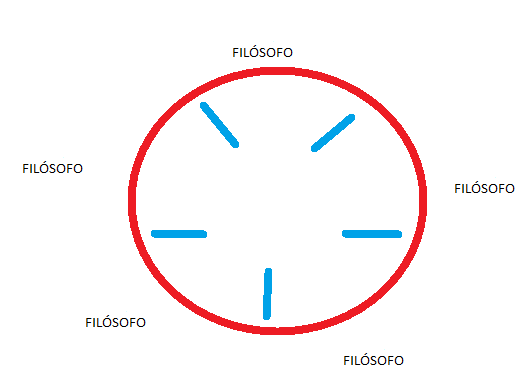
\includegraphics{Filosofos.png}
\caption{Esquema de los filósofos}\end{figure}


\subsection{Boceto de solución}
\label{textos/tema2:boceto-de-solucion}
\begin{Verbatim}[commandchars=\\\{\}]
\PYG{k+kn}{import} \PYG{n+nn}{java.util.Random}\PYG{o}{;}


\PYG{k+kd}{public} \PYG{k+kd}{class} \PYG{n+nc}{Filosofo}  \PYG{k+kd}{implements} \PYG{n}{Runnable}\PYG{o}{\PYGZob{}}
        \PYG{k+kd}{public} \PYG{k+kt}{void} \PYG{n+nf}{run}\PYG{o}{(}\PYG{o}{)}\PYG{o}{\PYGZob{}}
                \PYG{n}{String} \PYG{n}{miNombre}\PYG{o}{=}\PYG{n}{Thread}\PYG{o}{.}\PYG{n+na}{currentThread}\PYG{o}{(}\PYG{o}{)}\PYG{o}{.}\PYG{n+na}{getName}\PYG{o}{(}\PYG{o}{)}\PYG{o}{;}
                \PYG{n}{Random} \PYG{n}{generador}\PYG{o}{=}\PYG{k}{new} \PYG{n}{Random}\PYG{o}{(}\PYG{o}{)}\PYG{o}{;}
                \PYG{k}{while} \PYG{o}{(}\PYG{k+kc}{true}\PYG{o}{)}\PYG{o}{\PYGZob{}}
                        \PYG{c+cm}{/* Comer*/}
                        \PYG{c+cm}{/* Intentar coger palillos*/}
                        \PYG{c+cm}{/* Si los coge:*/}
                        \PYG{n}{System}\PYG{o}{.}\PYG{n+na}{out}\PYG{o}{.}\PYG{n+na}{println}\PYG{o}{(}\PYG{n}{miNombre}\PYG{o}{+}\PYG{l+s}{\PYGZdq{} comiendo...\PYGZdq{}}\PYG{o}{)}\PYG{o}{;}
                        \PYG{k+kt}{int} \PYG{n}{milisegs}\PYG{o}{=}\PYG{o}{(}\PYG{l+m+mi}{1}\PYG{o}{+}\PYG{n}{generador}\PYG{o}{.}\PYG{n+na}{nextInt}\PYG{o}{(}\PYG{l+m+mi}{5}\PYG{o}{)}\PYG{o}{)}\PYG{o}{*}\PYG{l+m+mi}{1000}\PYG{o}{;}
                        \PYG{n}{esperarTiempoAzar}\PYG{o}{(}\PYG{n}{miNombre}\PYG{o}{,} \PYG{n}{milisegs}\PYG{o}{)}\PYG{o}{;}
                        \PYG{c+cm}{/* Pensando...*/}
                        \PYG{c+c1}{//Recordemos soltar los palillos}
                        \PYG{n}{System}\PYG{o}{.}\PYG{n+na}{out}\PYG{o}{.}\PYG{n+na}{println}\PYG{o}{(}\PYG{n}{miNombre}\PYG{o}{+}\PYG{l+s}{\PYGZdq{}  pensando...\PYGZdq{}}\PYG{o}{)}\PYG{o}{;}                           \PYG{n}{milisegs}\PYG{o}{=}\PYG{o}{(}\PYG{l+m+mi}{1}\PYG{o}{+}\PYG{n}{generador}\PYG{o}{.}\PYG{n+na}{nextInt}\PYG{o}{(}\PYG{l+m+mi}{5}\PYG{o}{)}\PYG{o}{)}\PYG{o}{*}\PYG{l+m+mi}{1000}\PYG{o}{;}
                        \PYG{n}{esperarTiempoAzar}\PYG{o}{(}\PYG{n}{miNombre}\PYG{o}{,} \PYG{n}{milisegs}\PYG{o}{)}\PYG{o}{;}
                \PYG{o}{\PYGZcb{}}
        \PYG{o}{\PYGZcb{}}

\PYG{k+kd}{private} \PYG{k+kt}{void} \PYG{n+nf}{esperarTiempoAzar}\PYG{o}{(}\PYG{n}{String} \PYG{n}{miNombre}\PYG{o}{,} \PYG{k+kt}{int} \PYG{n}{milisegs}\PYG{o}{)} \PYG{o}{\PYGZob{}}
                \PYG{k}{try} \PYG{o}{\PYGZob{}}
                        \PYG{n}{Thread}\PYG{o}{.}\PYG{n+na}{sleep}\PYG{o}{(}\PYG{n}{milisegs}\PYG{o}{)}\PYG{o}{;}
                \PYG{o}{\PYGZcb{}} \PYG{k}{catch} \PYG{o}{(}\PYG{n}{InterruptedException} \PYG{n}{e}\PYG{o}{)} \PYG{o}{\PYGZob{}}
                        \PYG{n}{System}\PYG{o}{.}\PYG{n+na}{out}\PYG{o}{.}\PYG{n+na}{println}\PYG{o}{(}
                                \PYG{n}{miNombre}\PYG{o}{+}\PYG{l+s}{\PYGZdq{} interrumpido!!. Saliendo...\PYGZdq{}}\PYG{o}{)}\PYG{o}{;}
                        \PYG{k}{return} \PYG{o}{;}
                \PYG{o}{\PYGZcb{}}
        \PYG{o}{\PYGZcb{}}
\PYG{o}{\PYGZcb{}}
\end{Verbatim}


\section{Solución completa al problema de los filósofos}
\label{textos/tema2:solucion-completa-al-problema-de-los-filosofos}

\subsection{Gestor de recursos compartidos (palillos)}
\label{textos/tema2:gestor-de-recursos-compartidos-palillos}
\begin{Verbatim}[commandchars=\\\{\}]
\PYG{k+kd}{public} \PYG{k+kd}{class} \PYG{n+nc}{GestorPalillos} \PYG{o}{\PYGZob{}}
        \PYG{c+cm}{/* False significa que no están cogidos*/}
        \PYG{k+kd}{private} \PYG{k+kt}{boolean}\PYG{o}{[}\PYG{o}{]} \PYG{n}{palillos}\PYG{o}{;}
        \PYG{k+kd}{public} \PYG{n+nf}{GestorPalillos}\PYG{o}{(}\PYG{k+kt}{int} \PYG{n}{num\PYGZus{}filosofos}\PYG{o}{)}\PYG{o}{\PYGZob{}}
                \PYG{n}{palillos}\PYG{o}{=}\PYG{k}{new} \PYG{k+kt}{boolean}\PYG{o}{[}\PYG{n}{num\PYGZus{}filosofos}\PYG{o}{]}\PYG{o}{;}
                \PYG{k}{for} \PYG{o}{(}\PYG{k+kt}{int} \PYG{n}{i}\PYG{o}{=}\PYG{l+m+mi}{0}\PYG{o}{;}\PYG{n}{i}\PYG{o}{\PYGZlt{}}\PYG{n}{palillos}\PYG{o}{.}\PYG{n+na}{length}\PYG{o}{;}\PYG{n}{i}\PYG{o}{+}\PYG{o}{+}\PYG{o}{)}\PYG{o}{\PYGZob{}}
                        \PYG{n}{palillos}\PYG{o}{[}\PYG{n}{i}\PYG{o}{]}\PYG{o}{=}\PYG{k+kc}{false}\PYG{o}{;}
                \PYG{o}{\PYGZcb{}}
        \PYG{o}{\PYGZcb{}}
        \PYG{k+kd}{public} \PYG{k+kd}{synchronized} \PYG{k+kt}{boolean}
                \PYG{n+nf}{sePuedenCogerAmbosPalillos}\PYG{o}{(}
                        \PYG{k+kt}{int} \PYG{n}{num1}\PYG{o}{,}\PYG{k+kt}{int} \PYG{n}{num2}\PYG{o}{)}\PYG{o}{\PYGZob{}}
                \PYG{k}{if} \PYG{o}{(} \PYG{o}{(}\PYG{n}{palillos}\PYG{o}{[}\PYG{n}{num1}\PYG{o}{]}\PYG{o}{=}\PYG{o}{=}\PYG{k+kc}{false}\PYG{o}{)} \PYG{o}{\PYGZam{}}\PYG{o}{\PYGZam{}}
                        \PYG{o}{(}\PYG{n}{palillos}\PYG{o}{[}\PYG{n}{num2}\PYG{o}{]}\PYG{o}{=}\PYG{o}{=}\PYG{k+kc}{false}\PYG{o}{)} \PYG{o}{)} \PYG{o}{\PYGZob{}}
                        \PYG{n}{palillos}\PYG{o}{[}\PYG{n}{num1}\PYG{o}{]}\PYG{o}{=}\PYG{k+kc}{true}\PYG{o}{;}
                        \PYG{n}{palillos}\PYG{o}{[}\PYG{n}{num2}\PYG{o}{]}\PYG{o}{=}\PYG{k+kc}{true}\PYG{o}{;}
                        \PYG{n}{System}\PYG{o}{.}\PYG{n+na}{out}\PYG{o}{.}\PYG{n+na}{println}\PYG{o}{(}
                                \PYG{l+s}{\PYGZdq{}Alguien consiguio los palillos \PYGZdq{}}
                                \PYG{o}{+}\PYG{n}{num1}\PYG{o}{+}\PYG{l+s}{\PYGZdq{} y \PYGZdq{}}\PYG{o}{+}\PYG{n}{num2}\PYG{o}{)}\PYG{o}{;}
                        \PYG{k}{return} \PYG{k+kc}{true}\PYG{o}{;}
                \PYG{o}{\PYGZcb{}}
                \PYG{k}{return} \PYG{k+kc}{false}\PYG{o}{;}
        \PYG{o}{\PYGZcb{}}
        \PYG{k+kd}{public} \PYG{k+kd}{synchronized} \PYG{k+kt}{void} \PYG{n+nf}{soltarPalillos}\PYG{o}{(}\PYG{k+kt}{int} \PYG{n}{num1}\PYG{o}{,} \PYG{k+kt}{int} \PYG{n}{num2}\PYG{o}{)}\PYG{o}{\PYGZob{}}
                \PYG{n}{palillos}\PYG{o}{[}\PYG{n}{num1}\PYG{o}{]}\PYG{o}{=}\PYG{k+kc}{false}\PYG{o}{;}
                \PYG{n}{palillos}\PYG{o}{[}\PYG{n}{num2}\PYG{o}{]}\PYG{o}{=}\PYG{k+kc}{false}\PYG{o}{;}
                \PYG{n}{System}\PYG{o}{.}\PYG{n+na}{out}\PYG{o}{.}\PYG{n+na}{println}\PYG{o}{(}
                        \PYG{l+s}{\PYGZdq{}Alguien liberó los palillos \PYGZdq{}}\PYG{o}{+}
                        \PYG{n}{num1}\PYG{o}{+}\PYG{l+s}{\PYGZdq{} y \PYGZdq{}}\PYG{o}{+}\PYG{n}{num2}\PYG{o}{)}\PYG{o}{;}
        \PYG{o}{\PYGZcb{}}
\PYG{o}{\PYGZcb{}}
\end{Verbatim}


\subsection{Simulación de un filósofo}
\label{textos/tema2:simulacion-de-un-filosofo}
\begin{Verbatim}[commandchars=\\\{\}]
\PYG{k+kn}{import} \PYG{n+nn}{java.util.Random}\PYG{o}{;}
\PYG{k+kd}{public} \PYG{k+kd}{class} \PYG{n+nc}{Filosofo}  \PYG{k+kd}{implements} \PYG{n}{Runnable}\PYG{o}{\PYGZob{}}
        \PYG{k+kt}{int} \PYG{n}{num\PYGZus{}palillo\PYGZus{}izq}\PYG{o}{;}
        \PYG{k+kt}{int} \PYG{n}{num\PYGZus{}palillo\PYGZus{}der}\PYG{o}{;}
        \PYG{n}{GestorPalillos} \PYG{n}{gestorPalillos}\PYG{o}{;}
        \PYG{k+kd}{public} \PYG{n+nf}{Filosofo}\PYG{o}{(}\PYG{n}{GestorPalillos} \PYG{n}{gp}\PYG{o}{,}
                        \PYG{k+kt}{int} \PYG{n}{p\PYGZus{}izq}\PYG{o}{,} \PYG{k+kt}{int} \PYG{n}{p\PYGZus{}der}\PYG{o}{)}\PYG{o}{\PYGZob{}}
                \PYG{k}{this}\PYG{o}{.}\PYG{n+na}{gestorPalillos}\PYG{o}{=}\PYG{n}{gp}\PYG{o}{;}
                \PYG{k}{this}\PYG{o}{.}\PYG{n+na}{num\PYGZus{}palillo\PYGZus{}der}\PYG{o}{=}\PYG{n}{p\PYGZus{}der}\PYG{o}{;}
                \PYG{k}{this}\PYG{o}{.}\PYG{n+na}{num\PYGZus{}palillo\PYGZus{}izq}\PYG{o}{=}\PYG{n}{p\PYGZus{}izq}\PYG{o}{;}
        \PYG{o}{\PYGZcb{}}
        \PYG{k+kd}{public} \PYG{k+kt}{void} \PYG{n+nf}{run}\PYG{o}{(}\PYG{o}{)}\PYG{o}{\PYGZob{}}
                \PYG{n}{String} \PYG{n}{miNombre}\PYG{o}{=}\PYG{n}{Thread}\PYG{o}{.}\PYG{n+na}{currentThread}\PYG{o}{(}\PYG{o}{)}\PYG{o}{.}\PYG{n+na}{getName}\PYG{o}{(}\PYG{o}{)}\PYG{o}{;}
                \PYG{n}{Random} \PYG{n}{generador}\PYG{o}{=}\PYG{k}{new} \PYG{n}{Random}\PYG{o}{(}\PYG{o}{)}\PYG{o}{;}
                \PYG{k}{while} \PYG{o}{(}\PYG{k+kc}{true}\PYG{o}{)}\PYG{o}{\PYGZob{}}
                        \PYG{c+cm}{/* Comer*/}
                        \PYG{c+cm}{/* Intentar coger palillos*/}
                        \PYG{k}{while}\PYG{o}{(}\PYG{o}{!}\PYG{n}{gestorPalillos}\PYG{o}{.}\PYG{n+na}{sePuedenCogerAmbosPalillos}
                                \PYG{o}{(}
                                                \PYG{n}{num\PYGZus{}palillo\PYGZus{}izq}\PYG{o}{,}
                                                \PYG{n}{num\PYGZus{}palillo\PYGZus{}der}
                                \PYG{o}{)}\PYG{o}{)}
                        \PYG{o}{\PYGZob{}}

                        \PYG{o}{\PYGZcb{}}
                        \PYG{c+cm}{/* Si los coge:*/}

                        \PYG{k+kt}{int} \PYG{n}{milisegs}\PYG{o}{=}\PYG{o}{(}\PYG{l+m+mi}{1}\PYG{o}{+}\PYG{n}{generador}\PYG{o}{.}\PYG{n+na}{nextInt}\PYG{o}{(}\PYG{l+m+mi}{5}\PYG{o}{)}\PYG{o}{)}\PYG{o}{*}\PYG{l+m+mi}{1000}\PYG{o}{;}
                        \PYG{n}{esperarTiempoAzar}\PYG{o}{(}\PYG{n}{miNombre}\PYG{o}{,} \PYG{n}{milisegs}\PYG{o}{)}\PYG{o}{;}
                        \PYG{c+cm}{/* Pensando...*/}
                        \PYG{c+c1}{//Recordemos soltar los palillos}
                        \PYG{n}{gestorPalillos}\PYG{o}{.}\PYG{n+na}{soltarPalillos}\PYG{o}{(}
                                \PYG{n}{num\PYGZus{}palillo\PYGZus{}izq}\PYG{o}{,}
                                \PYG{n}{num\PYGZus{}palillo\PYGZus{}der}\PYG{o}{)}\PYG{o}{;}

                        \PYG{n}{milisegs}\PYG{o}{=}\PYG{o}{(}\PYG{l+m+mi}{1}\PYG{o}{+}\PYG{n}{generador}\PYG{o}{.}\PYG{n+na}{nextInt}\PYG{o}{(}\PYG{l+m+mi}{5}\PYG{o}{)}\PYG{o}{)}\PYG{o}{*}\PYG{l+m+mi}{1000}\PYG{o}{;}
                        \PYG{n}{esperarTiempoAzar}\PYG{o}{(}\PYG{n}{miNombre}\PYG{o}{,} \PYG{n}{milisegs}\PYG{o}{)}\PYG{o}{;}
                \PYG{o}{\PYGZcb{}}
        \PYG{o}{\PYGZcb{}}

\PYG{k+kd}{private} \PYG{k+kt}{void} \PYG{n+nf}{esperarTiempoAzar}\PYG{o}{(}\PYG{n}{String} \PYG{n}{miNombre}\PYG{o}{,} \PYG{k+kt}{int} \PYG{n}{milisegs}\PYG{o}{)} \PYG{o}{\PYGZob{}}
                \PYG{k}{try} \PYG{o}{\PYGZob{}}
                        \PYG{n}{Thread}\PYG{o}{.}\PYG{n+na}{sleep}\PYG{o}{(}\PYG{n}{milisegs}\PYG{o}{)}\PYG{o}{;}
                \PYG{o}{\PYGZcb{}} \PYG{k}{catch} \PYG{o}{(}\PYG{n}{InterruptedException} \PYG{n}{e}\PYG{o}{)} \PYG{o}{\PYGZob{}}
                        \PYG{n}{System}\PYG{o}{.}\PYG{n+na}{out}\PYG{o}{.}\PYG{n+na}{println}\PYG{o}{(}
                                \PYG{n}{miNombre}\PYG{o}{+}
                                \PYG{l+s}{\PYGZdq{} interrumpido!!. Saliendo...\PYGZdq{}}\PYG{o}{)}\PYG{o}{;}
                        \PYG{k}{return} \PYG{o}{;}
                \PYG{o}{\PYGZcb{}}
        \PYG{o}{\PYGZcb{}}
\PYG{o}{\PYGZcb{}}
\end{Verbatim}


\subsection{Lanzador de hilos}
\label{textos/tema2:lanzador-de-hilos}
\begin{Verbatim}[commandchars=\\\{\}]
\PYG{k+kd}{public} \PYG{k+kd}{class} \PYG{n+nc}{LanzadorFilosofos} \PYG{o}{\PYGZob{}}
        \PYG{k+kd}{public} \PYG{k+kd}{static} \PYG{k+kt}{void} \PYG{n+nf}{main}\PYG{o}{(}\PYG{n}{String}\PYG{o}{[}\PYG{o}{]} \PYG{n}{args}\PYG{o}{)} \PYG{o}{\PYGZob{}}
                \PYG{k+kt}{int} \PYG{n}{MAX\PYGZus{}FILOSOFOS}\PYG{o}{=}\PYG{l+m+mi}{5}\PYG{o}{;}
                \PYG{n}{Filosofo}\PYG{o}{[}\PYG{o}{]} \PYG{n}{filosofos}\PYG{o}{=}\PYG{k}{new} \PYG{n}{Filosofo}\PYG{o}{[}\PYG{n}{MAX\PYGZus{}FILOSOFOS}\PYG{o}{]}\PYG{o}{;}
                \PYG{n}{Thread}\PYG{o}{[}\PYG{o}{]} \PYG{n}{hilosAsociados}\PYG{o}{=}\PYG{k}{new} \PYG{n}{Thread}\PYG{o}{[}\PYG{n}{MAX\PYGZus{}FILOSOFOS}\PYG{o}{]}\PYG{o}{;}
                \PYG{n}{GestorPalillos} \PYG{n}{gestorCompartido}\PYG{o}{=}
                                \PYG{k}{new} \PYG{n+nf}{GestorPalillos}\PYG{o}{(}\PYG{n}{MAX\PYGZus{}FILOSOFOS}\PYG{o}{)}\PYG{o}{;}
                \PYG{k}{for} \PYG{o}{(}\PYG{k+kt}{int} \PYG{n}{i}\PYG{o}{=}\PYG{l+m+mi}{0}\PYG{o}{;} \PYG{n}{i}\PYG{o}{\PYGZlt{}}\PYG{n}{MAX\PYGZus{}FILOSOFOS}\PYG{o}{;} \PYG{n}{i}\PYG{o}{+}\PYG{o}{+}\PYG{o}{)}\PYG{o}{\PYGZob{}}
                        \PYG{k}{if} \PYG{o}{(}\PYG{n}{i}\PYG{o}{=}\PYG{o}{=}\PYG{l+m+mi}{0}\PYG{o}{)}\PYG{o}{\PYGZob{}}
                                \PYG{n}{filosofos}\PYG{o}{[}\PYG{n}{i}\PYG{o}{]}\PYG{o}{=}
                                \PYG{k}{new} \PYG{n+nf}{Filosofo}\PYG{o}{(}
                                                \PYG{n}{gestorCompartido}\PYG{o}{,}
                                                \PYG{n}{i}\PYG{o}{,}\PYG{n}{MAX\PYGZus{}FILOSOFOS}\PYG{o}{\PYGZhy{}}\PYG{l+m+mi}{1}\PYG{o}{)}\PYG{o}{;}
                        \PYG{o}{\PYGZcb{}}
                        \PYG{k}{else} \PYG{o}{\PYGZob{}}
                                \PYG{n}{filosofos}\PYG{o}{[}\PYG{n}{i}\PYG{o}{]}\PYG{o}{=}\PYG{k}{new} \PYG{n}{Filosofo}\PYG{o}{(}
                                                \PYG{n}{gestorCompartido}\PYG{o}{,} \PYG{n}{i}\PYG{o}{,} \PYG{n}{i}\PYG{o}{\PYGZhy{}}\PYG{l+m+mi}{1}\PYG{o}{)}\PYG{o}{;}
                        \PYG{o}{\PYGZcb{}}
                        \PYG{n}{Thread} \PYG{n}{hilo}\PYG{o}{=}\PYG{k}{new} \PYG{n}{Thread}\PYG{o}{(}\PYG{n}{filosofos}\PYG{o}{[}\PYG{n}{i}\PYG{o}{]}\PYG{o}{)}\PYG{o}{;}
                        \PYG{n}{hilo}\PYG{o}{.}\PYG{n+na}{setName}\PYG{o}{(}\PYG{l+s}{\PYGZdq{}Filosofo \PYGZdq{}}\PYG{o}{+}\PYG{n}{i}\PYG{o}{)}\PYG{o}{;}
                        \PYG{n}{hilosAsociados}\PYG{o}{[}\PYG{n}{i}\PYG{o}{]}\PYG{o}{=}\PYG{n}{hilo}\PYG{o}{;}
                        \PYG{n}{hilo}\PYG{o}{.}\PYG{n+na}{start}\PYG{o}{(}\PYG{o}{)}\PYG{o}{;}
                \PYG{o}{\PYGZcb{}}
                \PYG{c+cm}{/* Un poco inútil*/}
                \PYG{k}{for} \PYG{o}{(}\PYG{k+kt}{int} \PYG{n}{i}\PYG{o}{=}\PYG{l+m+mi}{0}\PYG{o}{;} \PYG{n}{i}\PYG{o}{\PYGZlt{}}\PYG{n}{MAX\PYGZus{}FILOSOFOS}\PYG{o}{;}\PYG{n}{i}\PYG{o}{+}\PYG{o}{+}\PYG{o}{)}\PYG{o}{\PYGZob{}}
                        \PYG{k}{try} \PYG{o}{\PYGZob{}}
                                \PYG{n}{hilosAsociados}\PYG{o}{[}\PYG{n}{i}\PYG{o}{]}\PYG{o}{.}\PYG{n+na}{join}\PYG{o}{(}\PYG{o}{)}\PYG{o}{;}
                        \PYG{o}{\PYGZcb{}} \PYG{k}{catch} \PYG{o}{(}\PYG{n}{InterruptedException} \PYG{n}{e}\PYG{o}{)} \PYG{o}{\PYGZob{}}
                                \PYG{c+c1}{// TODO Auto\PYGZhy{}generated catch block}
                                \PYG{n}{e}\PYG{o}{.}\PYG{n+na}{printStackTrace}\PYG{o}{(}\PYG{o}{)}\PYG{o}{;}
                        \PYG{o}{\PYGZcb{}}
                \PYG{o}{\PYGZcb{}}
        \PYG{o}{\PYGZcb{}}
\PYG{o}{\PYGZcb{}}
\end{Verbatim}


\section{Problema}
\label{textos/tema2:id1}
En una peluquería hay barberos y sillas para los clientes (siempre hay más sillas que clientes). Sin embargo, en esta peluquería no siempre hay trabajo por lo que los barberos duermen cuando no hay clientes a los que afeitar. Un cliente puede llegar a la barbería y encontrar alguna silla libre, en cuyo caso, el cliente se sienta y esperará que algún barbero le afeite. Puede ocurrir que el cliente llegue y no haya sillas libres, en cuyo caso se marcha. Simular el comportamiento de la barbería mediante un programa Java.
\begin{figure}[htbp]
\centering
\capstart

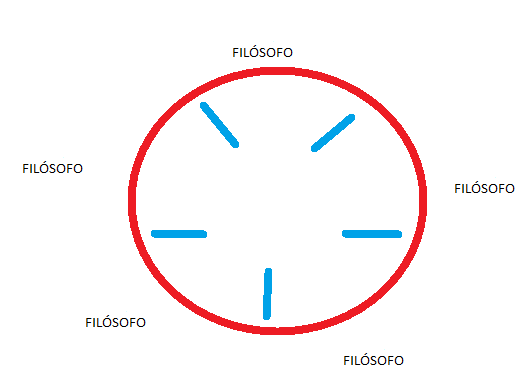
\includegraphics{barberodormilon.png}
\caption{Los  barberos dormilones}\end{figure}


\section{Una (mala) solución al problema de los barberos}
\label{textos/tema2:una-mala-solucion-al-problema-de-los-barberos}
Prueba la siguiente solución:


\subsection{Clase Barbero}
\label{textos/tema2:clase-barbero}
\begin{Verbatim}[commandchars=\\\{\}]
\PYG{k+kd}{public} \PYG{k+kd}{class} \PYG{n+nc}{Barbero} \PYG{k+kd}{implements} \PYG{n}{Runnable} \PYG{o}{\PYGZob{}}
        \PYG{k+kd}{private} \PYG{n}{String}                          \PYG{n}{nombre}\PYG{o}{;}
        \PYG{k+kd}{private} \PYG{n}{GestorConcurrencia}      \PYG{n}{gc}\PYG{o}{;}
        \PYG{k+kd}{private} \PYG{n}{Random}                          \PYG{n}{generador}\PYG{o}{;}
        \PYG{k+kd}{private} \PYG{k+kt}{int}                                     \PYG{n}{MAX\PYGZus{}ESPERA\PYGZus{}SEGS}\PYG{o}{=}\PYG{l+m+mi}{5}\PYG{o}{;}
        \PYG{k+kd}{public} \PYG{n+nf}{Barbero}\PYG{o}{(}\PYG{n}{GestorConcurrencia} \PYG{n}{gc}\PYG{o}{,}\PYG{n}{String} \PYG{n}{nombre}\PYG{o}{)}\PYG{o}{\PYGZob{}}
                \PYG{k}{this}\PYG{o}{.}\PYG{n+na}{nombre}             \PYG{o}{=}\PYG{n}{nombre}\PYG{o}{;}
                \PYG{k}{this}\PYG{o}{.}\PYG{n+na}{gc}                 \PYG{o}{=}\PYG{n}{gc}\PYG{o}{;}
                \PYG{k}{this}\PYG{o}{.}\PYG{n+na}{generador}  \PYG{o}{=}\PYG{k}{new} \PYG{n}{Random}\PYG{o}{(}\PYG{o}{)}\PYG{o}{;}
        \PYG{o}{\PYGZcb{}}

        \PYG{k+kd}{public} \PYG{k+kt}{void} \PYG{n+nf}{esperarTiempoAzar}\PYG{o}{(}\PYG{k+kt}{int} \PYG{n}{max}\PYG{o}{)}\PYG{o}{\PYGZob{}}
                \PYG{c+cm}{/* Se calculan unos milisegundos al azar*/}
                \PYG{k+kt}{int} \PYG{n}{msgs}\PYG{o}{=}\PYG{o}{(}\PYG{l+m+mi}{1}\PYG{o}{+}\PYG{n}{generador}\PYG{o}{.}\PYG{n+na}{nextInt}\PYG{o}{(}\PYG{n}{max}\PYG{o}{)}\PYG{o}{)}\PYG{o}{*}\PYG{l+m+mi}{1000}\PYG{o}{;}
                \PYG{k}{try} \PYG{o}{\PYGZob{}}
                        \PYG{n}{Thread}\PYG{o}{.}\PYG{n+na}{currentThread}\PYG{o}{(}\PYG{o}{)}\PYG{o}{.}\PYG{n+na}{sleep}\PYG{o}{(}\PYG{n}{msgs}\PYG{o}{)}\PYG{o}{;}
                \PYG{o}{\PYGZcb{}} \PYG{k}{catch} \PYG{o}{(}\PYG{n}{InterruptedException} \PYG{n}{e}\PYG{o}{)} \PYG{o}{\PYGZob{}}
                        \PYG{c+c1}{// TODO Auto\PYGZhy{}generated catch block}
                        \PYG{n}{e}\PYG{o}{.}\PYG{n+na}{printStackTrace}\PYG{o}{(}\PYG{o}{)}\PYG{o}{;}
                \PYG{o}{\PYGZcb{}}
        \PYG{o}{\PYGZcb{}}
        \PYG{k+kd}{public} \PYG{k+kt}{void} \PYG{n+nf}{run}\PYG{o}{(}\PYG{o}{)}\PYG{o}{\PYGZob{}}
                \PYG{k}{while} \PYG{o}{(}\PYG{k+kc}{true}\PYG{o}{)}\PYG{o}{\PYGZob{}}
                        \PYG{k+kt}{int} \PYG{n}{num\PYGZus{}silla}\PYG{o}{=}\PYG{n}{gc}\PYG{o}{.}\PYG{n+na}{atenderAlgunCliente}\PYG{o}{(}\PYG{o}{)}\PYG{o}{;}
                        \PYG{k}{while} \PYG{o}{(}\PYG{n}{num\PYGZus{}silla}\PYG{o}{=}\PYG{o}{=}\PYG{o}{\PYGZhy{}}\PYG{l+m+mi}{1}\PYG{o}{)}\PYG{o}{\PYGZob{}}
                                \PYG{c+cm}{/* Mientras no haya nadie a quien}
\PYG{c+cm}{                                 * atender, dormimos}
\PYG{c+cm}{                                 */}
                                \PYG{n}{esperarTiempoAzar}\PYG{o}{(}\PYG{n}{MAX\PYGZus{}ESPERA\PYGZus{}SEGS}\PYG{o}{)}\PYG{o}{;}
                                \PYG{n}{num\PYGZus{}silla}\PYG{o}{=}\PYG{n}{gc}\PYG{o}{.}\PYG{n+na}{atenderAlgunCliente}\PYG{o}{(}\PYG{o}{)}\PYG{o}{;}
                        \PYG{o}{\PYGZcb{}}
                        \PYG{c+cm}{/* Si llegamos aqui es que había algún cliente}
\PYG{c+cm}{                         * Simulamos un tiempo de afeitado}
\PYG{c+cm}{                         */}
                        \PYG{n}{esperarTiempoAzar}\PYG{o}{(}\PYG{n}{MAX\PYGZus{}ESPERA\PYGZus{}SEGS}\PYG{o}{)}\PYG{o}{;}
                        \PYG{c+cm}{/* Tras ese tiempo de afeitado se}
\PYG{c+cm}{                         * libera la silla}
\PYG{c+cm}{                         */}
                        \PYG{n}{gc}\PYG{o}{.}\PYG{n+na}{liberarSilla}\PYG{o}{(}\PYG{n}{num\PYGZus{}silla}\PYG{o}{)}\PYG{o}{;}
                        \PYG{c+cm}{/* Y vuelta a empezar*/}
                \PYG{o}{\PYGZcb{}}
        \PYG{o}{\PYGZcb{}}
\PYG{o}{\PYGZcb{}}
\end{Verbatim}


\subsection{Clase Cliente}
\label{textos/tema2:clase-cliente}
\begin{Verbatim}[commandchars=\\\{\}]
\PYG{k+kd}{public} \PYG{k+kd}{class} \PYG{n+nc}{Cliente} \PYG{k+kd}{implements} \PYG{n}{Runnable}\PYG{o}{\PYGZob{}}
        \PYG{n}{GestorConcurrencia}      \PYG{n}{gc}\PYG{o}{;}
        \PYG{k+kd}{public} \PYG{n+nf}{Cliente}\PYG{o}{(}\PYG{n}{GestorConcurrencia} \PYG{n}{gc}\PYG{o}{)}\PYG{o}{\PYGZob{}}
                \PYG{k}{this}\PYG{o}{.}\PYG{n+na}{gc}         \PYG{o}{=}\PYG{n}{gc}\PYG{o}{;}
        \PYG{o}{\PYGZcb{}}
        \PYG{k+kd}{public} \PYG{k+kt}{void} \PYG{n+nf}{run}\PYG{o}{(}\PYG{o}{)}\PYG{o}{\PYGZob{}}
                \PYG{c+cm}{/* Los clientes no esperan que haya}
\PYG{c+cm}{                 * sillas libres, no hay bucle infinito.}
\PYG{c+cm}{                 * Si no hay sillas libres se van...}
\PYG{c+cm}{                 */}
                \PYG{n}{gc}\PYG{o}{.}\PYG{n+na}{getSillaLibre}\PYG{o}{(}\PYG{o}{)}\PYG{o}{;}
        \PYG{o}{\PYGZcb{}}
\PYG{o}{\PYGZcb{}}
\end{Verbatim}


\subsection{Clase GestorConcurrencia}
\label{textos/tema2:clase-gestorconcurrencia}
\begin{Verbatim}[commandchars=\\\{\}]
\PYG{k+kd}{public} \PYG{k+kd}{class} \PYG{n+nc}{GestorConcurrencia} \PYG{o}{\PYGZob{}}
        \PYG{c+cm}{/* Vector que indica cuantas sillas hay y}
\PYG{c+cm}{         * si están libres o no}
\PYG{c+cm}{         */}
        \PYG{k+kt}{boolean}\PYG{o}{[}\PYG{o}{]} \PYG{n}{sillasLibres}\PYG{o}{;}
        \PYG{c+cm}{/* Indica si el cliente sentado en esa}
\PYG{c+cm}{         * silla está atendido por un barbero o no}
\PYG{c+cm}{         */}
        \PYG{k+kt}{boolean}\PYG{o}{[}\PYG{o}{]} \PYG{n}{clienteEstaAtendido}\PYG{o}{;}

        \PYG{k+kd}{public} \PYG{n+nf}{GestorConcurrencia}\PYG{o}{(}\PYG{k+kt}{int} \PYG{n}{numSillas}\PYG{o}{)}\PYG{o}{\PYGZob{}}
                \PYG{c+cm}{/*Construimos los vectores...*/}
                \PYG{n}{sillasLibres}            \PYG{o}{=}\PYG{k}{new} \PYG{k+kt}{boolean}\PYG{o}{[}\PYG{n}{numSillas}\PYG{o}{]}\PYG{o}{;}
                \PYG{n}{clienteEstaAtendido}     \PYG{o}{=}\PYG{k}{new} \PYG{k+kt}{boolean}\PYG{o}{[}\PYG{n}{numSillas}\PYG{o}{]}\PYG{o}{;}
                \PYG{c+cm}{/* ... los inicializamos*/}
                \PYG{k}{for} \PYG{o}{(}\PYG{k+kt}{int} \PYG{n}{i}\PYG{o}{=}\PYG{l+m+mi}{0}\PYG{o}{;} \PYG{n}{i}\PYG{o}{\PYGZlt{}}\PYG{n}{numSillas}\PYG{o}{;}\PYG{n}{i}\PYG{o}{+}\PYG{o}{+}\PYG{o}{)}\PYG{o}{\PYGZob{}}
                        \PYG{n}{sillasLibres}\PYG{o}{[}\PYG{n}{i}\PYG{o}{]}                 \PYG{o}{=}\PYG{k+kc}{true}\PYG{o}{;}
                        \PYG{n}{clienteEstaAtendido}\PYG{o}{[}\PYG{n}{i}\PYG{o}{]}  \PYG{o}{=}\PYG{k+kc}{false}\PYG{o}{;}
                \PYG{o}{\PYGZcb{}}
        \PYG{o}{\PYGZcb{}}

        \PYG{c+cm}{/**}
\PYG{c+cm}{         * Permite obtener una silla libre, usado por la}
\PYG{c+cm}{         * clase Cliente para saber si puede sentarse}
\PYG{c+cm}{         * en algún sitio o irse}
\PYG{c+cm}{         * @return Devuelve el número de la primera silla}
\PYG{c+cm}{         * que está libre o \PYGZhy{}1 si no hay ninguna}
\PYG{c+cm}{         */}
        \PYG{k+kd}{public} \PYG{k+kd}{synchronized} \PYG{k+kt}{int} \PYG{n+nf}{getSillaLibre}\PYG{o}{(}\PYG{o}{)}\PYG{o}{\PYGZob{}}
                \PYG{k}{for} \PYG{o}{(}\PYG{k+kt}{int} \PYG{n}{i}\PYG{o}{=}\PYG{l+m+mi}{0}\PYG{o}{;} \PYG{n}{i}\PYG{o}{\PYGZlt{}}\PYG{n}{sillasLibres}\PYG{o}{.}\PYG{n+na}{length}\PYG{o}{;} \PYG{n}{i}\PYG{o}{+}\PYG{o}{+}\PYG{o}{)}\PYG{o}{\PYGZob{}}
                        \PYG{c+cm}{/* Si está libre la silla ...*/}
                        \PYG{k}{if} \PYG{o}{(}\PYG{n}{sillasLibres}\PYG{o}{[}\PYG{n}{i}\PYG{o}{]}\PYG{o}{)} \PYG{o}{\PYGZob{}}
                                \PYG{c+cm}{/* ...se marca como ocupada*/}
                                \PYG{n}{sillasLibres}\PYG{o}{[}\PYG{n}{i}\PYG{o}{]}\PYG{o}{=}\PYG{k+kc}{false}\PYG{o}{;}
                                \PYG{n}{System}\PYG{o}{.}\PYG{n+na}{out}\PYG{o}{.}\PYG{n+na}{println}\PYG{o}{(}
                                        \PYG{l+s}{\PYGZdq{}Cliente sentado en silla \PYGZdq{}}\PYG{o}{+}\PYG{n}{i}
                                                \PYG{o}{)}\PYG{o}{;}
                                \PYG{c+cm}{/*.. y devolvemos i...*/}
                                \PYG{k}{return} \PYG{n}{i}\PYG{o}{;}
                        \PYG{o}{\PYGZcb{}}
                \PYG{o}{\PYGZcb{}}
                \PYG{c+cm}{/* Si llegamos aquí es que no había nada libre*/}
                \PYG{k}{return} \PYG{o}{\PYGZhy{}}\PYG{l+m+mi}{1}\PYG{o}{;}
        \PYG{o}{\PYGZcb{}}

        \PYG{c+cm}{/**}
\PYG{c+cm}{         * Nos dice qué silla tiene algun cliente}
\PYG{c+cm}{         * que no está atendido}
\PYG{c+cm}{         * @return un número de silla o \PYGZhy{}1 si no}
\PYG{c+cm}{         * hay clientes sin atender}
\PYG{c+cm}{         */}
        \PYG{k+kd}{public} \PYG{k+kd}{synchronized} \PYG{k+kt}{int} \PYG{n+nf}{atenderAlgunCliente}\PYG{o}{(}\PYG{o}{)}\PYG{o}{\PYGZob{}}
                \PYG{k}{for} \PYG{o}{(}\PYG{k+kt}{int} \PYG{n}{i}\PYG{o}{=}\PYG{l+m+mi}{0}\PYG{o}{;} \PYG{n}{i}\PYG{o}{\PYGZlt{}}\PYG{n}{sillasLibres}\PYG{o}{.}\PYG{n+na}{length}\PYG{o}{;} \PYG{n}{i}\PYG{o}{+}\PYG{o}{+}\PYG{o}{)}\PYG{o}{\PYGZob{}}
                        \PYG{c+cm}{/* Si una silla está ocupada (no libre, false)}
\PYG{c+cm}{                         * y está marcado como \PYGZdq{}sin atender\PYGZdq{} (false)}
\PYG{c+cm}{                         * entonces la marcamos como atendida}
\PYG{c+cm}{                         */}
                        \PYG{k}{if} \PYG{o}{(}\PYG{n}{clienteEstaAtendido}\PYG{o}{[}\PYG{n}{i}\PYG{o}{]}\PYG{o}{=}\PYG{o}{=}\PYG{k+kc}{false}\PYG{o}{)}\PYG{o}{\PYGZob{}}
                                \PYG{n}{clienteEstaAtendido}\PYG{o}{[}\PYG{n}{i}\PYG{o}{]}\PYG{o}{=}\PYG{k+kc}{true}\PYG{o}{;}
                                \PYG{n}{System}\PYG{o}{.}\PYG{n+na}{out}\PYG{o}{.}\PYG{n+na}{println}\PYG{o}{(}
                                                \PYG{l+s}{\PYGZdq{}Afeitando cliente en silla \PYGZdq{}}\PYG{o}{+}\PYG{n}{i}\PYG{o}{)}\PYG{o}{;}
                                \PYG{k}{return} \PYG{n}{i}\PYG{o}{;}
                        \PYG{o}{\PYGZcb{}}
                \PYG{o}{\PYGZcb{}}
                \PYG{k}{return} \PYG{o}{\PYGZhy{}}\PYG{l+m+mi}{1}\PYG{o}{;}
        \PYG{o}{\PYGZcb{}}

        \PYG{c+cm}{/* El cliente de esa silla, se marcha, por lo}
\PYG{c+cm}{         * que se marca esa silla como \PYGZdq{}libre\PYGZdq{}}
\PYG{c+cm}{         * y como \PYGZdq{}sin atender\PYGZdq{}}
\PYG{c+cm}{         */}
        \PYG{k+kd}{public} \PYG{k+kd}{synchronized} \PYG{k+kt}{void} \PYG{n+nf}{liberarSilla}\PYG{o}{(}\PYG{k+kt}{int} \PYG{n}{i}\PYG{o}{)}\PYG{o}{\PYGZob{}}
                \PYG{n}{sillasLibres}\PYG{o}{[}\PYG{n}{i}\PYG{o}{]}                 \PYG{o}{=}\PYG{k+kc}{true}\PYG{o}{;}
                \PYG{n}{clienteEstaAtendido}\PYG{o}{[}\PYG{n}{i}\PYG{o}{]}  \PYG{o}{=}\PYG{k+kc}{false}\PYG{o}{;}
                \PYG{n}{System}\PYG{o}{.}\PYG{n+na}{out}\PYG{o}{.}\PYG{n+na}{println}\PYG{o}{(}
                                \PYG{l+s}{\PYGZdq{}Se marcha el cliente de la silla \PYGZdq{}}\PYG{o}{+}\PYG{n}{i}\PYG{o}{)}\PYG{o}{;}
        \PYG{o}{\PYGZcb{}}
\PYG{o}{\PYGZcb{}}
\end{Verbatim}


\subsection{Clase Lanzador}
\label{textos/tema2:clase-lanzador}
\begin{Verbatim}[commandchars=\\\{\}]
\PYG{k+kd}{public} \PYG{k+kd}{class} \PYG{n+nc}{Lanzador} \PYG{o}{\PYGZob{}}

        \PYG{k+kd}{public} \PYG{k+kd}{static} \PYG{k+kt}{void} \PYG{n+nf}{main}\PYG{o}{(}\PYG{n}{String}\PYG{o}{[}\PYG{o}{]} \PYG{n}{args}\PYG{o}{)} \PYG{o}{\PYGZob{}}

                \PYG{k+kt}{int} \PYG{n}{MAX\PYGZus{}BARBEROS}        \PYG{o}{=}\PYG{l+m+mi}{2}\PYG{o}{;}
                \PYG{k+kt}{int} \PYG{n}{MAX\PYGZus{}SILLAS}          \PYG{o}{=}\PYG{n}{MAX\PYGZus{}BARBEROS}\PYG{o}{+}\PYG{l+m+mi}{1}\PYG{o}{;}
                \PYG{k+kt}{int} \PYG{n}{MAX\PYGZus{}CLIENTES}        \PYG{o}{=}\PYG{n}{MAX\PYGZus{}BARBEROS}\PYG{o}{*}\PYG{l+m+mi}{10}\PYG{o}{;}
                \PYG{k+kt}{int} \PYG{n}{MAX\PYGZus{}ESPERA\PYGZus{}SEGS}     \PYG{o}{=} \PYG{l+m+mi}{3}\PYG{o}{;}
                \PYG{n}{GestorConcurrencia} \PYG{n}{gc}\PYG{o}{;}
                \PYG{n}{gc}\PYG{o}{=}\PYG{k}{new} \PYG{n}{GestorConcurrencia}\PYG{o}{(}\PYG{n}{MAX\PYGZus{}SILLAS}\PYG{o}{)}\PYG{o}{;}

                \PYG{n}{Thread}\PYG{o}{[}\PYG{o}{]} \PYG{n}{vhBarberos}     \PYG{o}{=}\PYG{k}{new} \PYG{n}{Thread}\PYG{o}{[}\PYG{n}{MAX\PYGZus{}BARBEROS}\PYG{o}{]}\PYG{o}{;}
                \PYG{k}{for} \PYG{o}{(}\PYG{k+kt}{int} \PYG{n}{i}\PYG{o}{=}\PYG{l+m+mi}{0}\PYG{o}{;} \PYG{n}{i}\PYG{o}{\PYGZlt{}}\PYG{n}{MAX\PYGZus{}BARBEROS}\PYG{o}{;}\PYG{n}{i}\PYG{o}{+}\PYG{o}{+}\PYG{o}{)}\PYG{o}{\PYGZob{}}
                        \PYG{n}{Barbero} \PYG{n}{b}\PYG{o}{=}\PYG{k}{new} \PYG{n}{Barbero}\PYG{o}{(}\PYG{n}{gc}\PYG{o}{,} \PYG{l+s}{\PYGZdq{}Barbero \PYGZdq{}}\PYG{o}{+}\PYG{n}{i}\PYG{o}{)}\PYG{o}{;}
                        \PYG{n}{Thread} \PYG{n}{hilo}\PYG{o}{=}\PYG{k}{new} \PYG{n}{Thread}\PYG{o}{(}\PYG{n}{b}\PYG{o}{)}\PYG{o}{;}
                        \PYG{n}{vhBarberos}\PYG{o}{[}\PYG{n}{i}\PYG{o}{]}\PYG{o}{=}\PYG{n}{hilo}\PYG{o}{;}
                        \PYG{n}{hilo}\PYG{o}{.}\PYG{n+na}{start}\PYG{o}{(}\PYG{o}{)}\PYG{o}{;}
                \PYG{o}{\PYGZcb{}}

                \PYG{c+cm}{/* Generamos unos cuantos clientes}
\PYG{c+cm}{                 * a intervalos aleatorios}
\PYG{c+cm}{                 */}
                \PYG{n}{Random} \PYG{n}{generador}\PYG{o}{=}\PYG{k}{new} \PYG{n}{Random}\PYG{o}{(}\PYG{o}{)}\PYG{o}{;}
                \PYG{k}{for} \PYG{o}{(}\PYG{k+kt}{int} \PYG{n}{i}\PYG{o}{=}\PYG{l+m+mi}{0}\PYG{o}{;} \PYG{n}{i}\PYG{o}{\PYGZlt{}}\PYG{n}{MAX\PYGZus{}CLIENTES}\PYG{o}{;} \PYG{n}{i}\PYG{o}{+}\PYG{o}{+}\PYG{o}{)}\PYG{o}{\PYGZob{}}
                        \PYG{n}{Cliente} \PYG{n}{c}                       \PYG{o}{=}\PYG{k}{new} \PYG{n}{Cliente}\PYG{o}{(}\PYG{n}{gc}\PYG{o}{)}\PYG{o}{;}
                        \PYG{n}{Thread} \PYG{n}{hiloCliente}      \PYG{o}{=}\PYG{k}{new} \PYG{n}{Thread}\PYG{o}{(}\PYG{n}{c}\PYG{o}{)}\PYG{o}{;}
                        \PYG{n}{hiloCliente}\PYG{o}{.}\PYG{n+na}{start}\PYG{o}{(}\PYG{o}{)}\PYG{o}{;}

                        \PYG{k+kt}{int} \PYG{n}{msegs}\PYG{o}{=}\PYG{n}{generador}\PYG{o}{.}\PYG{n+na}{nextInt}\PYG{o}{(}\PYG{l+m+mi}{3}\PYG{o}{)}\PYG{o}{*}\PYG{l+m+mi}{1000}\PYG{o}{;}
                        \PYG{k}{try} \PYG{o}{\PYGZob{}}
                                \PYG{n}{Thread}\PYG{o}{.}\PYG{n+na}{sleep}\PYG{o}{(}\PYG{n}{msegs}\PYG{o}{)}\PYG{o}{;}
                        \PYG{o}{\PYGZcb{}} \PYG{k}{catch} \PYG{o}{(}\PYG{n}{InterruptedException} \PYG{n}{e}\PYG{o}{)} \PYG{o}{\PYGZob{}}
                                \PYG{c+c1}{// TODO Auto\PYGZhy{}generated catch block}
                                \PYG{n}{e}\PYG{o}{.}\PYG{n+na}{printStackTrace}\PYG{o}{(}\PYG{o}{)}\PYG{o}{;}
                        \PYG{o}{\PYGZcb{}}
                \PYG{o}{\PYGZcb{}} \PYG{c+cm}{/* Fin del for*/}
        \PYG{o}{\PYGZcb{}}
\PYG{o}{\PYGZcb{}}
\end{Verbatim}


\subsection{Críticas a la solución anterior}
\label{textos/tema2:criticas-a-la-solucion-anterior}
¿Cual es el problema?

El problema está en que la forma que tiene el gestor de concurrencia de decirle a un barbero qué silla tiene un cliente sin afeitar es incorrecta: como siempre se empieza a buscar por el principio del vector, los clientes sentados al final \textbf{nunca son atendidos}. Hay que corregir esa asignación para \emph{evitar que los procesos sufrán de inanición}.


\subsection{Método corregido}
\label{textos/tema2:metodo-corregido}
\begin{Verbatim}[commandchars=\\\{\}]
\PYG{k+kd}{public} \PYG{k+kd}{synchronized} \PYG{k+kt}{int} \PYG{n+nf}{atenderAlgunCliente}\PYG{o}{(}\PYG{o}{)}\PYG{o}{\PYGZob{}}
        \PYG{k}{for} \PYG{o}{(}\PYG{k+kt}{int} \PYG{n}{pasos}\PYG{o}{=}\PYG{l+m+mi}{0}\PYG{o}{;}
                        \PYG{n}{pasos}\PYG{o}{\PYGZlt{}}\PYG{n}{clienteEstaAtendido}\PYG{o}{.}\PYG{n+na}{length}\PYG{o}{;}
                        \PYG{n}{pasos}\PYG{o}{+}\PYG{o}{+}\PYG{o}{)}
        \PYG{o}{\PYGZob{}}
                \PYG{k}{if} \PYG{o}{(}
                                \PYG{n}{clienteEstaAtendido}
                                \PYG{o}{[}\PYG{n}{numUltimaSillaExaminada}\PYG{o}{]}
                                                \PYG{o}{=}\PYG{o}{=} \PYG{k+kc}{false}
                                                \PYG{o}{)}
                \PYG{o}{\PYGZob{}}
                        \PYG{c+cm}{/*Atendemos a ese cliente*/}
                        \PYG{n}{clienteEstaAtendido}
                                \PYG{o}{[}\PYG{n}{numUltimaSillaExaminada}\PYG{o}{]}\PYG{o}{=}\PYG{k+kc}{true}\PYG{o}{;}
                        \PYG{n}{System}\PYG{o}{.}\PYG{n+na}{out}\PYG{o}{.}\PYG{n+na}{println}\PYG{o}{(}
                                        \PYG{l+s}{\PYGZdq{}Afeitando cliente en silla \PYGZdq{}}\PYG{o}{+}
                                                        \PYG{n}{numUltimaSillaExaminada}\PYG{o}{)}\PYG{o}{;}
                        \PYG{k}{return} \PYG{n}{numUltimaSillaExaminada}\PYG{o}{;}
                \PYG{o}{\PYGZcb{}} \PYG{k}{else} \PYG{o}{\PYGZob{}}
                        \PYG{n}{numUltimaSillaExaminada}\PYG{o}{=}
                                        \PYG{o}{(}\PYG{n}{numUltimaSillaExaminada}\PYG{o}{+}\PYG{l+m+mi}{1}\PYG{o}{)}\PYG{o}{\PYGZpc{}}
                                        \PYG{n}{clienteEstaAtendido}\PYG{o}{.}\PYG{n+na}{length}\PYG{o}{;}
                \PYG{o}{\PYGZcb{}} \PYG{c+c1}{//Fin del else}
        \PYG{o}{\PYGZcb{}} \PYG{c+c1}{//Fin del for}
        \PYG{c+cm}{/* Si llegamos aquí hemos dado toda}
\PYG{c+cm}{         * una vuelta al vector y no había nadie sin}
\PYG{c+cm}{         * atender devolver \PYGZhy{}1}
\PYG{c+cm}{         */}
        \PYG{k}{return} \PYG{o}{\PYGZhy{}}\PYG{l+m+mi}{1}\PYG{o}{;}
\PYG{o}{\PYGZcb{}} \PYG{c+c1}{//Fin del método}
\end{Verbatim}


\section{Problema: productores y consumidores.}
\label{textos/tema2:problema-productores-y-consumidores}
En un cierto programa se tienen procesos que producen números y procesos que leen esos números. Todos los números se introducen en una cola (o vector) limitada.

Todo el mundo lee y escribe de/en esa cola. Cuando un productor quiere poner un número tendrá que comprobar si la cola está llena. Si está llena, espera un tiempo al azar. Si no está llena pone su número en la última posición libre.

Cuando un lector quiere leer, examina si la cola está vacía. Si lo está espera un tiempo al azar, y sino coge el número que haya al principio de la cola y ese número \emph{ya no está disponible para el siguiente}.

Crear un programa que simule el comportamiento de estos procesos evitando problemas de entrelazado e inanición.


\section{Solución}
\label{textos/tema2:solucion}

\subsection{Una cola limitada en tamaño}
\label{textos/tema2:una-cola-limitada-en-tamano}
\begin{Verbatim}[commandchars=\\\{\}]
\PYG{k+kd}{public} \PYG{k+kd}{class} \PYG{n+nc}{ColaLimitada} \PYG{o}{\PYGZob{}}
        \PYG{k+kt}{int}\PYG{o}{[}\PYG{o}{]} \PYG{n}{cola}\PYG{o}{;}
        \PYG{k+kt}{int} \PYG{n}{posParaEncolar}\PYG{o}{;}
        \PYG{k+kd}{public} \PYG{n+nf}{ColaLimitada}\PYG{o}{(}\PYG{k+kt}{int} \PYG{n}{numElementos}\PYG{o}{)}\PYG{o}{\PYGZob{}}
                \PYG{n}{cola}\PYG{o}{=}\PYG{k}{new} \PYG{k+kt}{int}\PYG{o}{[}\PYG{n}{numElementos}\PYG{o}{]}\PYG{o}{;}
                \PYG{n}{posParaEncolar}\PYG{o}{=}\PYG{l+m+mi}{0}\PYG{o}{;}
        \PYG{o}{\PYGZcb{}}
        \PYG{k+kd}{public} \PYG{k+kt}{void} \PYG{n+nf}{ponerEnCola}\PYG{o}{(}\PYG{k+kt}{int} \PYG{n}{numero}\PYG{o}{)}\PYG{o}{\PYGZob{}}
                \PYG{k}{if} \PYG{o}{(}\PYG{n}{posParaEncolar}\PYG{o}{=}\PYG{o}{=}\PYG{n}{cola}\PYG{o}{.}\PYG{n+na}{length}\PYG{o}{)}\PYG{o}{\PYGZob{}}
                        \PYG{n}{System}\PYG{o}{.}\PYG{n+na}{out}\PYG{o}{.}\PYG{n+na}{println}\PYG{o}{(}
                                        \PYG{l+s}{\PYGZdq{}Cola llena, debe Vd. esperar\PYGZdq{}}\PYG{o}{)}\PYG{o}{;}
                        \PYG{c+c1}{//Cola llena.}
                        \PYG{k}{return} \PYG{o}{;}
                \PYG{o}{\PYGZcb{}}
                \PYG{c+c1}{//Aún queda sitio}
                \PYG{n}{cola}\PYG{o}{[}\PYG{n}{posParaEncolar}\PYG{o}{]}\PYG{o}{=}\PYG{n}{numero}\PYG{o}{;}
                \PYG{n}{posParaEncolar}\PYG{o}{+}\PYG{o}{+}\PYG{o}{;}
        \PYG{o}{\PYGZcb{}}
        \PYG{k+kd}{public} \PYG{k+kt}{int} \PYG{n+nf}{sacarPrimero}\PYG{o}{(}\PYG{o}{)}\PYG{o}{\PYGZob{}}
                \PYG{k}{if} \PYG{o}{(}\PYG{n}{posParaEncolar}\PYG{o}{=}\PYG{o}{=}\PYG{l+m+mi}{0}\PYG{o}{)}\PYG{o}{\PYGZob{}}
                        \PYG{n}{System}\PYG{o}{.}\PYG{n+na}{out}\PYG{o}{.}\PYG{n+na}{println}\PYG{o}{(}
                                        \PYG{l+s}{\PYGZdq{}Warning:cola vacía, devolviendo 0\PYGZdq{}}
                        \PYG{o}{)}\PYG{o}{;}
                        \PYG{k}{return} \PYG{l+m+mi}{0}\PYG{o}{;}
                \PYG{o}{\PYGZcb{}}
                \PYG{k+kt}{int} \PYG{n}{elementoInicial}\PYG{o}{=}\PYG{n}{cola}\PYG{o}{[}\PYG{l+m+mi}{0}\PYG{o}{]}\PYG{o}{;}
                \PYG{c+cm}{/*Movemos los elementos hacia delante*/}
                \PYG{k}{for} \PYG{o}{(}\PYG{k+kt}{int} \PYG{n}{pos}\PYG{o}{=}\PYG{l+m+mi}{1}\PYG{o}{;} \PYG{n}{pos}\PYG{o}{\PYGZlt{}}\PYG{n}{cola}\PYG{o}{.}\PYG{n+na}{length}\PYG{o}{;} \PYG{n}{pos}\PYG{o}{+}\PYG{o}{+}\PYG{o}{)}\PYG{o}{\PYGZob{}}
                        \PYG{n}{cola}\PYG{o}{[}\PYG{n}{pos}\PYG{o}{\PYGZhy{}}\PYG{l+m+mi}{1}\PYG{o}{]}\PYG{o}{=}\PYG{n}{cola}\PYG{o}{[}\PYG{n}{pos}\PYG{o}{]}\PYG{o}{;}
                \PYG{o}{\PYGZcb{}}
                \PYG{c+cm}{/* Ahora la posParaEncolar ha disminuido*/}
                \PYG{n}{posParaEncolar}\PYG{o}{\PYGZhy{}}\PYG{o}{\PYGZhy{}}\PYG{o}{;}
                \PYG{k}{return} \PYG{n}{elementoInicial}\PYG{o}{;}
        \PYG{o}{\PYGZcb{}}
        \PYG{k+kd}{public} \PYG{n}{String} \PYG{n+nf}{toString}\PYG{o}{(}\PYG{o}{)}\PYG{o}{\PYGZob{}}
                \PYG{n}{String} \PYG{n}{cadenaCola}\PYG{o}{=}\PYG{l+s}{\PYGZdq{}\PYGZdq{}}\PYG{o}{;}
                \PYG{k}{for} \PYG{o}{(}\PYG{k+kt}{int} \PYG{n}{pos}\PYG{o}{=}\PYG{l+m+mi}{0}\PYG{o}{;} \PYG{n}{pos}\PYG{o}{\PYGZlt{}}\PYG{n}{posParaEncolar}\PYG{o}{;} \PYG{n}{pos}\PYG{o}{+}\PYG{o}{+}\PYG{o}{)}\PYG{o}{\PYGZob{}}
                        \PYG{n}{cadenaCola}\PYG{o}{+}\PYG{o}{=}\PYG{n}{cola}\PYG{o}{[}\PYG{n}{pos}\PYG{o}{]}\PYG{o}{+}\PYG{l+s}{\PYGZdq{}\PYGZhy{}\PYGZdq{}}\PYG{o}{;}
                \PYG{o}{\PYGZcb{}}
                \PYG{n}{cadenaCola}\PYG{o}{+}\PYG{o}{=}\PYG{l+s}{\PYGZdq{}FIN\PYGZdq{}}\PYG{o}{;}
                \PYG{k}{return} \PYG{n}{cadenaCola}\PYG{o}{;}
        \PYG{o}{\PYGZcb{}}
\PYG{o}{\PYGZcb{}}
\end{Verbatim}


\subsection{Un gestor de concurrencia para la cola}
\label{textos/tema2:un-gestor-de-concurrencia-para-la-cola}
\begin{Verbatim}[commandchars=\\\{\}]
\PYG{k+kd}{public} \PYG{k+kd}{class} \PYG{n+nc}{GestorColasConcurrentes} \PYG{o}{\PYGZob{}}
        \PYG{k+kd}{private} \PYG{n}{ColaLimitada} \PYG{n}{colaProtegida}\PYG{o}{;}
        \PYG{k+kd}{public} \PYG{n+nf}{GestorColasConcurrentes}\PYG{o}{(}\PYG{k+kt}{int} \PYG{n}{numElementos}\PYG{o}{)}\PYG{o}{\PYGZob{}}
                \PYG{n}{colaProtegida}\PYG{o}{=}\PYG{k}{new} \PYG{n}{ColaLimitada}\PYG{o}{(}\PYG{n}{numElementos}\PYG{o}{)}\PYG{o}{;}
        \PYG{o}{\PYGZcb{}}
        \PYG{k+kd}{public} \PYG{k+kd}{synchronized}
                \PYG{k+kt}{void} \PYG{n+nf}{ponerEnCola}\PYG{o}{(}\PYG{k+kt}{int} \PYG{n}{elemento}\PYG{o}{)}\PYG{o}{\PYGZob{}}
                \PYG{n}{colaProtegida}\PYG{o}{.}\PYG{n+na}{ponerEnCola}\PYG{o}{(}\PYG{n}{elemento}\PYG{o}{)}\PYG{o}{;}
        \PYG{o}{\PYGZcb{}}
        \PYG{k+kd}{public} \PYG{k+kd}{synchronized} \PYG{k+kt}{int} \PYG{n+nf}{sacarDeCola}\PYG{o}{(}\PYG{o}{)}\PYG{o}{\PYGZob{}}
                \PYG{k}{return} \PYG{n}{colaProtegida}\PYG{o}{.}\PYG{n+na}{sacarPrimero}\PYG{o}{(}\PYG{o}{)}\PYG{o}{;}
        \PYG{o}{\PYGZcb{}}
\PYG{o}{\PYGZcb{}}
\end{Verbatim}


\subsection{La clase Productor}
\label{textos/tema2:la-clase-productor}
\begin{Verbatim}[commandchars=\\\{\}]
\PYG{k+kd}{public} \PYG{k+kd}{class} \PYG{n+nc}{Productor} \PYG{k+kd}{implements} \PYG{n}{Runnable}\PYG{o}{\PYGZob{}}
        \PYG{k+kd}{private} \PYG{n}{Random}                                                  \PYG{n}{generadorAzar}\PYG{o}{;}
        \PYG{k+kd}{private}         \PYG{n}{GestorColasConcurrentes}         \PYG{n}{gc}\PYG{o}{;}
        \PYG{k+kd}{public} \PYG{n+nf}{Productor}\PYG{o}{(}\PYG{n}{GestorColasConcurrentes} \PYG{n}{gc}\PYG{o}{)}\PYG{o}{\PYGZob{}}
                \PYG{k}{this}\PYG{o}{.}\PYG{n+na}{gc}\PYG{o}{=}\PYG{n}{gc}\PYG{o}{;}
                \PYG{k}{this}\PYG{o}{.}\PYG{n+na}{generadorAzar}\PYG{o}{=}\PYG{k}{new} \PYG{n}{Random}\PYG{o}{(}\PYG{o}{)}\PYG{o}{;}
        \PYG{o}{\PYGZcb{}}
        \PYG{k+kd}{public} \PYG{k+kt}{void} \PYG{n+nf}{run}\PYG{o}{(}\PYG{o}{)}\PYG{o}{\PYGZob{}}
                \PYG{k}{while} \PYG{o}{(}\PYG{k+kc}{true}\PYG{o}{)}\PYG{o}{\PYGZob{}}
                        \PYG{k+kt}{int} \PYG{n}{numero}\PYG{o}{=}\PYG{n}{generadorAzar}\PYG{o}{.}\PYG{n+na}{nextInt}\PYG{o}{(}\PYG{l+m+mi}{20}\PYG{o}{)}\PYG{o}{;}
                        \PYG{n}{gc}\PYG{o}{.}\PYG{n+na}{ponerEnCola}\PYG{o}{(}\PYG{n}{numero}\PYG{o}{)}\PYG{o}{;}
                        \PYG{k+kt}{int} \PYG{n}{milisegs}\PYG{o}{=}\PYG{n}{generadorAzar}\PYG{o}{.}\PYG{n+na}{nextInt}\PYG{o}{(}\PYG{l+m+mi}{2}\PYG{o}{)}\PYG{o}{;}
                        \PYG{k}{try} \PYG{o}{\PYGZob{}}
                                \PYG{n}{Thread}\PYG{o}{.}\PYG{n+na}{currentThread}\PYG{o}{(}\PYG{o}{)}\PYG{o}{.}\PYG{n+na}{sleep}\PYG{o}{(}\PYG{n}{milisegs}\PYG{o}{*}\PYG{l+m+mi}{1000}\PYG{o}{)}\PYG{o}{;}
                        \PYG{o}{\PYGZcb{}} \PYG{k}{catch} \PYG{o}{(}\PYG{n}{InterruptedException} \PYG{n}{e}\PYG{o}{)} \PYG{o}{\PYGZob{}}
                                \PYG{n}{System}\PYG{o}{.}\PYG{n+na}{out}\PYG{o}{.}\PYG{n+na}{println}\PYG{o}{(}
                                                \PYG{l+s}{\PYGZdq{}Productor interrumpido\PYGZdq{}}
                                \PYG{o}{)}\PYG{o}{;}
                                \PYG{k}{return}\PYG{o}{;}
                        \PYG{o}{\PYGZcb{}}
                \PYG{o}{\PYGZcb{}}
        \PYG{o}{\PYGZcb{}}
\PYG{o}{\PYGZcb{}}
\end{Verbatim}


\subsection{La clase consumidor}
\label{textos/tema2:la-clase-consumidor}
\begin{Verbatim}[commandchars=\\\{\}]
\PYG{k+kd}{public} \PYG{k+kd}{class} \PYG{n+nc}{Consumidor} \PYG{k+kd}{implements} \PYG{n}{Runnable} \PYG{o}{\PYGZob{}}
        \PYG{k+kd}{private} \PYG{n}{Random}                                                  \PYG{n}{generadorAzar}\PYG{o}{;}
        \PYG{k+kd}{private} \PYG{n}{GestorColasConcurrentes}         \PYG{n}{gc}\PYG{o}{;}

        \PYG{k+kd}{public} \PYG{n+nf}{Consumidor}\PYG{o}{(}\PYG{n}{GestorColasConcurrentes} \PYG{n}{gc}\PYG{o}{)}\PYG{o}{\PYGZob{}}
                \PYG{k}{this}\PYG{o}{.}\PYG{n+na}{gc}\PYG{o}{=}\PYG{n}{gc}\PYG{o}{;}
                \PYG{k}{this}\PYG{o}{.}\PYG{n+na}{generadorAzar}\PYG{o}{=}\PYG{k}{new} \PYG{n}{Random}\PYG{o}{(}\PYG{o}{)}\PYG{o}{;}
        \PYG{o}{\PYGZcb{}}
        \PYG{k+kd}{public} \PYG{k+kt}{void} \PYG{n+nf}{run}\PYG{o}{(}\PYG{o}{)}\PYG{o}{\PYGZob{}}
                \PYG{k}{while} \PYG{o}{(}\PYG{k+kc}{true}\PYG{o}{)}\PYG{o}{\PYGZob{}}
                        \PYG{k+kt}{int} \PYG{n}{num}\PYG{o}{=}\PYG{n}{gc}\PYG{o}{.}\PYG{n+na}{sacarDeCola}\PYG{o}{(}\PYG{o}{)}\PYG{o}{;}
                        \PYG{k+kt}{int} \PYG{n}{milisegs}\PYG{o}{=}\PYG{n}{generadorAzar}\PYG{o}{.}\PYG{n+na}{nextInt}\PYG{o}{(}\PYG{l+m+mi}{2}\PYG{o}{)}\PYG{o}{;}
                        \PYG{k}{try} \PYG{o}{\PYGZob{}}
                                \PYG{n}{Thread}\PYG{o}{.}\PYG{n+na}{currentThread}\PYG{o}{(}\PYG{o}{)}\PYG{o}{.}\PYG{n+na}{sleep}\PYG{o}{(}\PYG{n}{milisegs}\PYG{o}{*}\PYG{l+m+mi}{1000}\PYG{o}{)}\PYG{o}{;}
                        \PYG{o}{\PYGZcb{}} \PYG{k}{catch} \PYG{o}{(}\PYG{n}{InterruptedException} \PYG{n}{e}\PYG{o}{)} \PYG{o}{\PYGZob{}}
                                \PYG{c+c1}{// TODO Auto\PYGZhy{}generated catch block}
                                \PYG{n}{System}\PYG{o}{.}\PYG{n+na}{out}\PYG{o}{.}\PYG{n+na}{println}\PYG{o}{(}
                                                \PYG{l+s}{\PYGZdq{}Consumidor interrumpido\PYGZdq{}}\PYG{o}{)}\PYG{o}{;}
                                \PYG{k}{return} \PYG{o}{;}
                        \PYG{o}{\PYGZcb{}}
                \PYG{o}{\PYGZcb{}}
        \PYG{o}{\PYGZcb{}}
\PYG{o}{\PYGZcb{}}
\end{Verbatim}


\subsection{Un lanzador}
\label{textos/tema2:un-lanzador}
\begin{Verbatim}[commandchars=\\\{\}]
\PYG{k+kd}{public} \PYG{k+kd}{class} \PYG{n+nc}{Lanzador} \PYG{o}{\PYGZob{}}
        \PYG{k+kd}{public} \PYG{k+kt}{void} \PYG{n+nf}{test}\PYG{o}{(}\PYG{o}{)}\PYG{o}{\PYGZob{}}
                \PYG{n}{ColaLimitada} \PYG{n}{c}\PYG{o}{=}\PYG{k}{new} \PYG{n}{ColaLimitada}\PYG{o}{(}\PYG{l+m+mi}{5}\PYG{o}{)}\PYG{o}{;}
                \PYG{k}{if} \PYG{o}{(}\PYG{n}{c}\PYG{o}{.}\PYG{n+na}{sacarPrimero}\PYG{o}{(}\PYG{o}{)}\PYG{o}{!}\PYG{o}{=}\PYG{l+m+mi}{0}\PYG{o}{)}\PYG{o}{\PYGZob{}}
                        \PYG{n}{System}\PYG{o}{.}\PYG{n+na}{out}\PYG{o}{.}\PYG{n+na}{println}\PYG{o}{(}
                          \PYG{l+s}{\PYGZdq{}Error, no se comprueba el caso cola vacía\PYGZdq{}}
                        \PYG{o}{)}\PYG{o}{;}
                \PYG{o}{\PYGZcb{}}
                \PYG{n}{c}\PYG{o}{.}\PYG{n+na}{ponerEnCola}\PYG{o}{(}\PYG{l+m+mi}{10}\PYG{o}{)}\PYG{o}{;}
                \PYG{n}{c}\PYG{o}{.}\PYG{n+na}{ponerEnCola}\PYG{o}{(}\PYG{l+m+mi}{20}\PYG{o}{)}\PYG{o}{;}
                \PYG{n}{String} \PYG{n}{cadenaCola}\PYG{o}{=}\PYG{n}{c}\PYG{o}{.}\PYG{n+na}{toString}\PYG{o}{(}\PYG{o}{)}\PYG{o}{;}
                \PYG{k}{if} \PYG{o}{(}\PYG{o}{!}\PYG{n}{cadenaCola}\PYG{o}{.}\PYG{n+na}{equals}\PYG{o}{(}\PYG{l+s}{\PYGZdq{}10\PYGZhy{}20\PYGZhy{}FIN\PYGZdq{}}\PYG{o}{)}\PYG{o}{)}\PYG{o}{\PYGZob{}}
                        \PYG{n}{System}\PYG{o}{.}\PYG{n+na}{out}\PYG{o}{.}\PYG{n+na}{println}\PYG{o}{(}\PYG{l+s}{\PYGZdq{}Fallos al encolar\PYGZdq{}}\PYG{o}{)}\PYG{o}{;}
                \PYG{o}{\PYGZcb{}}
        \PYG{o}{\PYGZcb{}}
        \PYG{k+kd}{public} \PYG{k+kd}{static} \PYG{k+kt}{void} \PYG{n+nf}{main}\PYG{o}{(}\PYG{n}{String}\PYG{o}{[}\PYG{o}{]} \PYG{n}{argumentos}\PYG{o}{)}\PYG{o}{\PYGZob{}}
                \PYG{n}{Lanzador} \PYG{n}{l}\PYG{o}{=}\PYG{k}{new} \PYG{n}{Lanzador}\PYG{o}{(}\PYG{o}{)}\PYG{o}{;}
                \PYG{n}{GestorColasConcurrentes} \PYG{n}{gcl}\PYG{o}{=}
                                \PYG{k}{new} \PYG{n+nf}{GestorColasConcurrentes}\PYG{o}{(}\PYG{l+m+mi}{10}\PYG{o}{)}\PYG{o}{;}

                \PYG{k+kt}{int} \PYG{n}{NUM\PYGZus{}PRODUCTORES}\PYG{o}{=}\PYG{l+m+mi}{5}\PYG{o}{;}
                \PYG{n}{Productor}\PYG{o}{[}\PYG{o}{]}     \PYG{n}{productores}\PYG{o}{;}
                \PYG{n}{Thread}\PYG{o}{[}\PYG{o}{]}                        \PYG{n}{hilosProductores}\PYG{o}{;}

                \PYG{n}{productores}             \PYG{o}{=}
                                \PYG{k}{new} \PYG{n}{Productor}\PYG{o}{[}\PYG{n}{NUM\PYGZus{}PRODUCTORES}\PYG{o}{]}\PYG{o}{;}
                \PYG{n}{hilosProductores}        \PYG{o}{=}
                                \PYG{k}{new} \PYG{n}{Thread}\PYG{o}{[}\PYG{n}{NUM\PYGZus{}PRODUCTORES}\PYG{o}{]}\PYG{o}{;}

                \PYG{k}{for} \PYG{o}{(}\PYG{k+kt}{int} \PYG{n}{i}\PYG{o}{=}\PYG{l+m+mi}{0}\PYG{o}{;} \PYG{n}{i}\PYG{o}{\PYGZlt{}}\PYG{n}{NUM\PYGZus{}PRODUCTORES}\PYG{o}{;} \PYG{n}{i}\PYG{o}{+}\PYG{o}{+}\PYG{o}{)}\PYG{o}{\PYGZob{}}
                        \PYG{n}{productores}\PYG{o}{[}\PYG{n}{i}\PYG{o}{]}\PYG{o}{=}\PYG{k}{new} \PYG{n}{Productor}\PYG{o}{(}\PYG{n}{gcl}\PYG{o}{)}\PYG{o}{;}
                        \PYG{n}{hilosProductores}\PYG{o}{[}\PYG{n}{i}\PYG{o}{]}\PYG{o}{=}\PYG{k}{new} \PYG{n}{Thread}\PYG{o}{(}
                                        \PYG{n}{productores}\PYG{o}{[}\PYG{n}{i}\PYG{o}{]}\PYG{o}{)}\PYG{o}{;}
                        \PYG{n}{hilosProductores}\PYG{o}{[}\PYG{n}{i}\PYG{o}{]}\PYG{o}{.}\PYG{n+na}{start}\PYG{o}{(}\PYG{o}{)}\PYG{o}{;}
                \PYG{o}{\PYGZcb{}}

                \PYG{k+kt}{int} \PYG{n}{NUM\PYGZus{}CONSUMIDORES}\PYG{o}{=}\PYG{l+m+mi}{10}\PYG{o}{;}
                \PYG{n}{Consumidor}\PYG{o}{[}\PYG{o}{]}    \PYG{n}{consumidores}\PYG{o}{;}
                \PYG{n}{Thread}\PYG{o}{[}\PYG{o}{]}                        \PYG{n}{hilosConsumidores}\PYG{o}{;}

                \PYG{n}{consumidores}                    \PYG{o}{=}
                                \PYG{k}{new} \PYG{n}{Consumidor}\PYG{o}{[}\PYG{n}{NUM\PYGZus{}CONSUMIDORES}\PYG{o}{]}\PYG{o}{;}
                \PYG{n}{hilosConsumidores}       \PYG{o}{=}
                                \PYG{k}{new} \PYG{n}{Thread}\PYG{o}{[}\PYG{n}{NUM\PYGZus{}CONSUMIDORES}\PYG{o}{]}\PYG{o}{;}


                \PYG{k}{for} \PYG{o}{(}\PYG{k+kt}{int} \PYG{n}{i}\PYG{o}{=}\PYG{l+m+mi}{0}\PYG{o}{;} \PYG{n}{i}\PYG{o}{\PYGZlt{}}\PYG{n}{NUM\PYGZus{}CONSUMIDORES}\PYG{o}{;} \PYG{n}{i}\PYG{o}{+}\PYG{o}{+}\PYG{o}{)}\PYG{o}{\PYGZob{}}
                        \PYG{n}{consumidores}\PYG{o}{[}\PYG{n}{i}\PYG{o}{]}\PYG{o}{=}\PYG{k}{new} \PYG{n}{Consumidor}\PYG{o}{(}\PYG{n}{gcl}\PYG{o}{)}\PYG{o}{;}
                        \PYG{n}{hilosConsumidores}\PYG{o}{[}\PYG{n}{i}\PYG{o}{]}\PYG{o}{=}
                                        \PYG{k}{new} \PYG{n+nf}{Thread}\PYG{o}{(}\PYG{n}{consumidores}\PYG{o}{[}\PYG{n}{i}\PYG{o}{]}\PYG{o}{)}\PYG{o}{;}
                        \PYG{n}{hilosConsumidores}\PYG{o}{[}\PYG{n}{i}\PYG{o}{]}\PYG{o}{.}\PYG{n+na}{start}\PYG{o}{(}\PYG{o}{)}\PYG{o}{;}
                \PYG{o}{\PYGZcb{}}

                \PYG{c+cm}{/* Se debería esperar a que todos terminen*/}
                \PYG{k}{for} \PYG{o}{(}\PYG{k+kt}{int} \PYG{n}{i}\PYG{o}{=}\PYG{l+m+mi}{0}\PYG{o}{;} \PYG{n}{i}\PYG{o}{\PYGZlt{}}\PYG{n}{NUM\PYGZus{}PRODUCTORES}\PYG{o}{;} \PYG{n}{i}\PYG{o}{+}\PYG{o}{+}\PYG{o}{)}\PYG{o}{\PYGZob{}}
                        \PYG{k}{try} \PYG{o}{\PYGZob{}}
                                \PYG{n}{hilosProductores}\PYG{o}{[}\PYG{n}{i}\PYG{o}{]}\PYG{o}{.}\PYG{n+na}{join}\PYG{o}{(}\PYG{o}{)}\PYG{o}{;}
                        \PYG{o}{\PYGZcb{}} \PYG{k}{catch} \PYG{o}{(}\PYG{n}{InterruptedException} \PYG{n}{e}\PYG{o}{)} \PYG{o}{\PYGZob{}}
                                \PYG{n}{e}\PYG{o}{.}\PYG{n+na}{printStackTrace}\PYG{o}{(}\PYG{o}{)}\PYG{o}{;}
                        \PYG{o}{\PYGZcb{}}
                \PYG{o}{\PYGZcb{}}
                \PYG{k}{for} \PYG{o}{(}\PYG{k+kt}{int} \PYG{n}{i}\PYG{o}{=}\PYG{l+m+mi}{0}\PYG{o}{;} \PYG{n}{i}\PYG{o}{\PYGZlt{}}\PYG{n}{NUM\PYGZus{}CONSUMIDORES}\PYG{o}{;} \PYG{n}{i}\PYG{o}{+}\PYG{o}{+}\PYG{o}{)}\PYG{o}{\PYGZob{}}
                        \PYG{k}{try} \PYG{o}{\PYGZob{}}
                                \PYG{n}{hilosConsumidores}\PYG{o}{[}\PYG{n}{i}\PYG{o}{]}\PYG{o}{.}\PYG{n+na}{join}\PYG{o}{(}\PYG{o}{)}\PYG{o}{;}
                        \PYG{o}{\PYGZcb{}} \PYG{k}{catch} \PYG{o}{(}\PYG{n}{InterruptedException} \PYG{n}{e}\PYG{o}{)} \PYG{o}{\PYGZob{}}
                                \PYG{c+c1}{// TODO Auto\PYGZhy{}generated catch block}
                                \PYG{n}{e}\PYG{o}{.}\PYG{n+na}{printStackTrace}\PYG{o}{(}\PYG{o}{)}\PYG{o}{;}
                        \PYG{o}{\PYGZcb{}}
                \PYG{o}{\PYGZcb{}}
        \PYG{o}{\PYGZcb{}}
\PYG{o}{\PYGZcb{}}
\end{Verbatim}


\section{Ejercicio}
\label{textos/tema2:ejercicio}
En unos grandes almacenes hay 300 clientes agolpados en la puerta para intentar conseguir un producto del cual solo hay 100 unidades.

Por la puerta solo cabe una persona, pero la paciencia de los clientes es limitada por lo que solo se harán un máximo de 10 intentos para entrar por la puerta. Si despues de 10 intentos la puerta no se ha encontrado libre ni una sola vez, el cliente desiste y se marcha.

Cuando se consigue entrar por la puerta el cliente puede encontrarse con dos situaciones:
\begin{enumerate}
\item {} 
Quedan productos: el cliente cogerá uno y se marchará.

\item {} 
No quedan productos: el cliente simplemente se marchará.

\end{enumerate}

Realizar la simulación en Java de dicha situación.


\section{Documentación.}
\label{textos/tema2:documentacion}

\section{Depuración.}
\label{textos/tema2:depuracion}

\chapter{Programación de comunicaciones en red}
\label{textos/tema3:programacion-de-comunicaciones-en-red}\label{textos/tema3::doc}

\section{Comunicación entre aplicaciones.}
\label{textos/tema3:comunicacion-entre-aplicaciones}
En Java toda la comunicación vista en primer curso de DAM consiste en dos cosas
\begin{itemize}
\item {} 
Entrada/salida por consola: con las clases \code{System.in} o \code{System.out}.

\item {} 
Lectura/escritura en ficheros: con las clases File y similares.

\end{itemize}

Se puede avanzar un paso más utilizando Java para enviar datos a través de Internet a otro programa Java remoto, que es lo que haremos en este capítulo.


\section{Roles cliente y servidor.}
\label{textos/tema3:roles-cliente-y-servidor}
Cuando se hacen programas Java que se comuniquen lo habitual es que uno o varios actúen de cliente y uno o varios actúen de servidores.
\begin{itemize}
\item {} 
Servidor: espera peticiones, recibe datos de entrada y devuelve respuestas.

\item {} 
Cliente: genera peticiones, las envía a un servidor y espera respuestas.

\end{itemize}

Un factor fundamental en los servidores es que tienen que ser capaces de procesar varias peticiones a la vez: \textbf{deben ser multihilo}.

Su arquitectura típica es la siguiente:

\begin{Verbatim}[commandchars=\\\{\}]
\PYG{k}{while} \PYG{o}{(}\PYG{k+kc}{true}\PYG{o}{)}\PYG{o}{\PYGZob{}}
        \PYG{n}{peticion}\PYG{o}{=}\PYG{n}{esperarPeticion}\PYG{o}{(}\PYG{o}{)}\PYG{o}{;}
        \PYG{n}{hiloAsociado}\PYG{o}{=}\PYG{k}{new} \PYG{n}{Hilo}\PYG{o}{(}\PYG{o}{)}\PYG{o}{;}
        \PYG{n}{hiloAsociado}\PYG{o}{.}\PYG{n+na}{atender}\PYG{o}{(}\PYG{n}{peticion}\PYG{o}{)}\PYG{o}{;}
\PYG{o}{\PYGZcb{}}
\end{Verbatim}


\section{Recordatorio de los flujos en Java}
\label{textos/tema3:recordatorio-de-los-flujos-en-java}

\subsection{InputStreams y OutputStreams}
\label{textos/tema3:inputstreams-y-outputstreams}
Manejan bytes a secas. Por ejemplo, si queremos leer un fichero byte a byte usaremos \code{FileInputStream} y si queremos escribir usaremos \code{FileOutputStream}.

Son operaciones a muy bajo nivel que usaremos muy pocas veces (por ejemplo, solo si quisiéramos cambiar el primer byte de un archivo). En general usaremos otras clases más cómodas de usar.


\subsection{Readers y Writers}
\label{textos/tema3:readers-y-writers}
En lugar de manejar \emph{bytes} manejan \emph{caracteres} (recordemos que hoy en día y con Unicode una letra como la \emph{ñ} en realidad podría ocupar más de un byte).

Así, cuando queramos leer letras de un archivo usaremos clases como \code{FileReader} y \code{FileWriter}.

Las clases \code{Readers} y \code{Writers} en realidad se apoyan sobre las \code{InputStreams} y \code{OutputStreams}.

A veces nos interesará mezclar conceptos y por ejemplo poder tener una clase que use caracteres cuando a lo mejor Java nos ha dado una clase que usa bytes. Así, por ejemplo \code{InputStreamReader} puede coger un objeto que lea bytes y nos devolverá caracteres. De la misma forma \code{OutputStreamWriter} coge letras y devuelve los bytes que la componen.


\subsection{\texttt{BufferedReaders} y \texttt{PrintWriters}}
\label{textos/tema3:bufferedreaders-y-printwriters}
Cuando trabajamos con caracteres (que recordemos pueden tener varios bytes) normalmente no trabajamos de uno en uno. Es más frecuente usar \textbf{líneas} que se leen y escriben de una sola vez. Así por ejemplo, la clase \code{PrintWriter} tiene un método \code{print(ln)} que puede imprimir elementos complejos como \code{floats} o cadenas largas.

Además, Java ofrece clases que gestionan automáticamente los \emph{buffers} por nosotros lo que nos da más comodidad y eficiencia. Por ello es muy habitual hacer cosas como esta:

\begin{Verbatim}[commandchars=\\\{\}]
\PYG{n}{lectorEficiente} \PYG{o}{=} \PYG{k}{new}
        \PYG{n}{BufferedReader}\PYG{o}{(}\PYG{k}{new} \PYG{n}{FileReader}\PYG{o}{(}\PYG{l+s}{\PYGZdq{}fich1.txt\PYGZdq{}}\PYG{o}{)}\PYG{o}{)}\PYG{o}{;}
\PYG{n}{escritorEficiente} \PYG{o}{=} \PYG{k}{new}
        \PYG{n}{BufferedWriter}\PYG{o}{(}\PYG{k}{new} \PYG{n}{FileWriter}\PYG{o}{(}\PYG{l+s}{\PYGZdq{}fich2.txt\PYGZdq{}}\PYG{o}{)}\PYG{o}{)}\PYG{o}{;}
\end{Verbatim}

En el primer caso creamos un objeto \code{FileReader} que es capaz de leer caracteres de \code{fich1.txt}. Como esto nos parece poco práctico creamos otro objeto a partir del primero de tipo \code{BufferedReader} que nos permitirá leer bloques enteros de texto.

De hecho, si se comprueba la ayuda de la clase \code{FileReader} se verá que solo hay un método \code{read} que devuelve un \code{int}, es decir el siguiente \textbf{carácter} disponible, lo que hace que el método sea muy incómodo. Sin embargo \code{BufferedReader}


\section{Elementos de programación de aplicaciones en red. Librerías.}
\label{textos/tema3:elementos-de-programacion-de-aplicaciones-en-red-librerias}
En Java toda la infraestructura de clases para trabajar con redes está en el paquete \code{java.net}.

En muchos casos nuestros programas empezarán con la sentencia \code{import java.net.*} pero muchos entornos (como Eclipse) son capaces de importar automáticamente las clases necesarias.


\subsection{La clase URL}
\label{textos/tema3:la-clase-url}
La clase URL permite gestionar accesos a URLs del tipo \code{http://marca.com/fichero.html} y descargar cosas con bastante sencillez.

Al crear un objeto URL se debe capturar la excepción \code{MalformedURLException} que sucede cuando hay algún error en la URL (como escribir \code{htp://marca.com}).

La clase URL nos ofrece un método \code{openStream} que nos devuelve un flujo básico de bytes. Podemos crear objetos más sofisticados para leer bloques como muestra el programa siguiente:

\begin{Verbatim}[commandchars=\\\{\}]
\PYG{k+kd}{public} \PYG{k+kd}{class} \PYG{n+nc}{GestorDescargas} \PYG{o}{\PYGZob{}}
        \PYG{k+kd}{public} \PYG{k+kt}{void} \PYG{n+nf}{descargarArchivo}\PYG{o}{(}
                        \PYG{n}{String} \PYG{n}{url\PYGZus{}descargar}\PYG{o}{,}
                        \PYG{n}{String} \PYG{n}{nombreArchivo}\PYG{o}{)}\PYG{o}{\PYGZob{}}
                \PYG{n}{System}\PYG{o}{.}\PYG{n+na}{out}\PYG{o}{.}\PYG{n+na}{println}\PYG{o}{(}\PYG{l+s}{\PYGZdq{}Descargando \PYGZdq{}}
                                \PYG{o}{+}\PYG{n}{url\PYGZus{}descargar}\PYG{o}{)}\PYG{o}{;}
                \PYG{k}{try} \PYG{o}{\PYGZob{}}
                        \PYG{n}{URL} \PYG{n}{laUrl}\PYG{o}{=}\PYG{k}{new} \PYG{n}{URL}\PYG{o}{(}\PYG{n}{url\PYGZus{}descargar}\PYG{o}{)}\PYG{o}{;}
                        \PYG{n}{InputStream} \PYG{n}{is}\PYG{o}{=}\PYG{n}{laUrl}\PYG{o}{.}\PYG{n+na}{openStream}\PYG{o}{(}\PYG{o}{)}\PYG{o}{;}
                        \PYG{n}{InputStreamReader} \PYG{n}{reader}\PYG{o}{=}
                                        \PYG{k}{new} \PYG{n+nf}{InputStreamReader}\PYG{o}{(}\PYG{n}{is}\PYG{o}{)}\PYG{o}{;}
                        \PYG{n}{BufferedReader} \PYG{n}{bReader}\PYG{o}{=}
                                        \PYG{k}{new} \PYG{n+nf}{BufferedReader}\PYG{o}{(}\PYG{n}{reader}\PYG{o}{)}\PYG{o}{;}
                        \PYG{n}{FileWriter} \PYG{n}{escritorFichero}\PYG{o}{=}
                                \PYG{k}{new} \PYG{n+nf}{FileWriter}\PYG{o}{(}\PYG{n}{nombreArchivo}\PYG{o}{)}\PYG{o}{;}
                        \PYG{n}{String} \PYG{n}{linea}\PYG{o}{;}
                        \PYG{k}{while} \PYG{o}{(}\PYG{o}{(}\PYG{n}{linea}\PYG{o}{=}\PYG{n}{bReader}\PYG{o}{.}\PYG{n+na}{readLine}\PYG{o}{(}\PYG{o}{)}\PYG{o}{)}\PYG{o}{!}\PYG{o}{=}\PYG{k+kc}{null}\PYG{o}{)}\PYG{o}{\PYGZob{}}
                                \PYG{n}{escritorFichero}\PYG{o}{.}\PYG{n+na}{write}\PYG{o}{(}\PYG{n}{linea}\PYG{o}{)}\PYG{o}{;}
                        \PYG{o}{\PYGZcb{}}
                        \PYG{n}{escritorFichero}\PYG{o}{.}\PYG{n+na}{close}\PYG{o}{(}\PYG{o}{)}\PYG{o}{;}
                        \PYG{n}{bReader}\PYG{o}{.}\PYG{n+na}{close}\PYG{o}{(}\PYG{o}{)}\PYG{o}{;}
                        \PYG{n}{reader}\PYG{o}{.}\PYG{n+na}{close}\PYG{o}{(}\PYG{o}{)}\PYG{o}{;}
                        \PYG{n}{is}\PYG{o}{.}\PYG{n+na}{close}\PYG{o}{(}\PYG{o}{)}\PYG{o}{;}
                \PYG{o}{\PYGZcb{}} \PYG{k}{catch} \PYG{o}{(}\PYG{n}{MalformedURLException} \PYG{n}{e}\PYG{o}{)} \PYG{o}{\PYGZob{}}
                        \PYG{n}{System}\PYG{o}{.}\PYG{n+na}{out}\PYG{o}{.}\PYG{n+na}{println}\PYG{o}{(}\PYG{l+s}{\PYGZdq{}URL mal escrita!\PYGZdq{}}\PYG{o}{)}\PYG{o}{;}
                        \PYG{k}{return} \PYG{o}{;}
                \PYG{o}{\PYGZcb{}} \PYG{k}{catch} \PYG{o}{(}\PYG{n}{IOException} \PYG{n}{e}\PYG{o}{)} \PYG{o}{\PYGZob{}}
                        \PYG{n}{System}\PYG{o}{.}\PYG{n+na}{out}\PYG{o}{.}\PYG{n+na}{println}\PYG{o}{(}
                                        \PYG{l+s}{\PYGZdq{}Fallo en la lectura del fichero\PYGZdq{}}\PYG{o}{)}\PYG{o}{;}
                        \PYG{k}{return} \PYG{o}{;}
                \PYG{o}{\PYGZcb{}}
        \PYG{o}{\PYGZcb{}}
        \PYG{k+kd}{public} \PYG{k+kd}{static} \PYG{k+kt}{void} \PYG{n+nf}{main} \PYG{o}{(}\PYG{n}{String}\PYG{o}{[}\PYG{o}{]} \PYG{n}{argumentos}\PYG{o}{)}\PYG{o}{\PYGZob{}}
                \PYG{n}{GestorDescargas} \PYG{n}{gd}\PYG{o}{=}\PYG{k}{new} \PYG{n}{GestorDescargas}\PYG{o}{(}\PYG{o}{)}\PYG{o}{;}
                \PYG{n}{String} \PYG{n}{base}\PYG{o}{=}
                        \PYG{l+s}{\PYGZdq{}http://10.13.0.20:8000\PYGZdq{}}\PYG{o}{+}
                                        \PYG{l+s}{\PYGZdq{}/ServiciosProcesos/textos/\PYGZdq{}}\PYG{o}{;}
                \PYG{k}{for} \PYG{o}{(}\PYG{k+kt}{int} \PYG{n}{i}\PYG{o}{=}\PYG{l+m+mi}{1}\PYG{o}{;} \PYG{n}{i}\PYG{o}{\PYGZlt{}}\PYG{o}{=}\PYG{l+m+mi}{5}\PYG{o}{;} \PYG{n}{i}\PYG{o}{+}\PYG{o}{+}\PYG{o}{)}\PYG{o}{\PYGZob{}}
                        \PYG{n}{String} \PYG{n}{url}\PYG{o}{=}\PYG{n}{base}\PYG{o}{+}\PYG{l+s}{\PYGZdq{}tema\PYGZdq{}}\PYG{o}{+}\PYG{n}{i}\PYG{o}{+}\PYG{l+s}{\PYGZdq{}.rst\PYGZdq{}}\PYG{o}{;}
                        \PYG{n}{gd}\PYG{o}{.}\PYG{n+na}{descargarArchivo}\PYG{o}{(}\PYG{n}{url}\PYG{o}{)}\PYG{o}{;}
                \PYG{o}{\PYGZcb{}}
        \PYG{o}{\PYGZcb{}}
\PYG{o}{\PYGZcb{}}
\end{Verbatim}


\section{Funciones y objetos de las librerías.}
\label{textos/tema3:funciones-y-objetos-de-las-librerias}
La clase URL proporciona un mecanismo muy sencillo pero por desgracia completamente atado al protocolo de las URL.

Java ofrece otros objetos que permiten tener un mayor control sobre lo que se envía o recibe a través de la red. Por desgracia esto implica que en muchos casos tendremos solo flujos de bajo nivel (streams).

En concreto Java ofrece dos elementos fundamentales para crear programas que usen redes
\begin{itemize}
\item {} 
Sockets

\item {} 
ServerSockets

\end{itemize}


\subsection{Repaso de redes}
\label{textos/tema3:repaso-de-redes}
En redes el protocolo IP es el responsable de dos cuestiones fundamentales:
\begin{itemize}
\item {} 
Establecer un sistema de direcciones universal (direcciones IP)

\item {} 
Establecer los mecanismos de enrutado.

\end{itemize}

Como programadores el segundo no nos interesa, pero el primero será absolutamente fundamental para contactar con programas que estén en una ubicación remota.

Una ubicación remota \emph{siempre} tendrá una dirección
IP pero \emph{solo a veces tendrá un nombre DNS}. Para nosotros no habrá diferencia ya que si es necesario el sistema operativo traducirá de nombre DNS a IP.

Otro elemento necesario en la comunicación en redes es el uso de un puerto de un cierto protocolo:
\begin{itemize}
\item {} 
TCP: ofrece fiabilidad a los programas.

\item {} 
UDP: ofrece velocidad sacrificando la fiabilidad.

\end{itemize}

A partir de ahora cuando usemos un número de puerto habrá que comprobar si ese número ya está usado.

Por ejemplo, es mala idea que nuestros programas usen el puerto 80 TCP, probablemente ya esté en uso.
Antes de usar un puerto en una aplicación comercial deberíamos consultar la lista de ``IANA assigned ports''.

En líneas generales se pueden usar los puertos desde 1024 TCP a 49151 TCP, pero deberíamos comprobar que el número que elegimos no sea un número usado por un puerto de alguna aplicación que haya en la empresa.

En las prácticas de clase usaremos el 9876 TCP. Si se desea conectar desde el instituto con algún programa ejecutado en casa se deberá ``abrir el puerto 9876 TCP''. Abrir un puerto consiste en configurar el router para que \textbf{SÍ ACEPTE TRÁFICO INICIADO DESDE EL EXTERIOR} cosa que no hace nunca por motivos de protección.


\section{Sockets.}
\label{textos/tema3:sockets}
Un \emph{socket} es un objeto Java que nos permite contactar con un programa o servidor remoto. Dicho objeto nos proporcionará flujos de entrada y/o salida y podremos comunicarnos con dicho programa.

Existe otro tipo de sockets, los \emph{ServerSocket}. Se utilizan para crear programas que acepten conexiones o peticiones.

Todos los objetos mencionados en este tema están en el paquete \code{java.net}.


\section{Creación de sockets.}
\label{textos/tema3:creacion-de-sockets}
En el siguiente código puede verse el proceso básico de creación de un socket. En los párrafos siguientes explicaremos el significado de los bloques de código.:

\begin{Verbatim}[commandchars=\\\{\}]
\PYG{k+kd}{public} \PYG{k+kd}{class} \PYG{n+nc}{Conector} \PYG{o}{\PYGZob{}}
        \PYG{k+kd}{public} \PYG{k+kd}{static} \PYG{k+kt}{void} \PYG{n+nf}{main}\PYG{o}{(}\PYG{n}{String}\PYG{o}{[}\PYG{o}{]} \PYG{n}{args}\PYG{o}{)} \PYG{o}{\PYGZob{}}
                \PYG{n}{String} \PYG{n}{destino}\PYG{o}{=}\PYG{l+s}{\PYGZdq{}www.google.com\PYGZdq{}}\PYG{o}{;}
                \PYG{k+kt}{int} \PYG{n}{puertoDestino}\PYG{o}{=}\PYG{l+m+mi}{80}\PYG{o}{;}
                \PYG{n}{Socket} \PYG{n}{socket}\PYG{o}{=}\PYG{k}{new} \PYG{n}{Socket}\PYG{o}{(}\PYG{o}{)}\PYG{o}{;}
                \PYG{n}{InetSocketAddress} \PYG{n}{direccion}\PYG{o}{=}\PYG{k}{new} \PYG{n}{InetSocketAddress}\PYG{o}{(}
                                \PYG{n}{destino}\PYG{o}{,} \PYG{n}{puertoDestino}\PYG{o}{)}\PYG{o}{;}
                \PYG{k}{try} \PYG{o}{\PYGZob{}}
                        \PYG{n}{socket}\PYG{o}{.}\PYG{n+na}{connect}\PYG{o}{(}\PYG{n}{direccion}\PYG{o}{)}\PYG{o}{;}
                        \PYG{c+c1}{//Si llegamos aquí es que la conexión}
                        \PYG{c+c1}{//sí se hizo.}

                        \PYG{n}{InputStream} \PYG{n}{is}\PYG{o}{=}\PYG{n}{socket}\PYG{o}{.}\PYG{n+na}{getInputStream}\PYG{o}{(}\PYG{o}{)}\PYG{o}{;}
                        \PYG{n}{OutputStream} \PYG{n}{os}\PYG{o}{=}\PYG{n}{socket}\PYG{o}{.}\PYG{n+na}{getOutputStream}\PYG{o}{(}\PYG{o}{)}\PYG{o}{;}


                \PYG{o}{\PYGZcb{}} \PYG{k}{catch} \PYG{o}{(}\PYG{n}{IOException} \PYG{n}{e}\PYG{o}{)} \PYG{o}{\PYGZob{}}
                        \PYG{n}{System}\PYG{o}{.}\PYG{n+na}{out}\PYG{o}{.}\PYG{n+na}{println}\PYG{o}{(}
                                \PYG{l+s}{\PYGZdq{}No se pudo establecer la conexion \PYGZdq{}}\PYG{o}{+}
                                \PYG{l+s}{\PYGZdq{} o hubo un fallo al leer datos.\PYGZdq{}}
                        \PYG{o}{)}\PYG{o}{;}
                \PYG{o}{\PYGZcb{}}
        \PYG{o}{\PYGZcb{}}
\PYG{o}{\PYGZcb{}}
\end{Verbatim}

Para poder crear un socket primero necesitamos una dirección con la que contactar. Toda dirección está formada por dirección IP (o DNS) y un puerto. En nuestro caso intentaremos contactar con \code{www.google.com:80}.

\begin{Verbatim}[commandchars=\\\{\}]
\PYG{n}{String} \PYG{n}{destino}\PYG{o}{=}\PYG{l+s}{\PYGZdq{}www.google.com\PYGZdq{}}\PYG{o}{;}
\PYG{k+kt}{int} \PYG{n}{puertoDestino}\PYG{o}{=}\PYG{l+m+mi}{80}\PYG{o}{;}
\PYG{n}{Socket} \PYG{n}{socket}\PYG{o}{=}\PYG{k}{new} \PYG{n}{Socket}\PYG{o}{(}\PYG{o}{)}\PYG{o}{;}
\PYG{n}{InetSocketAddress} \PYG{n}{direccion}\PYG{o}{=}\PYG{k}{new}
        \PYG{n}{InetSocketAddress}\PYG{o}{(}
                        \PYG{n}{destino}\PYG{o}{,} \PYG{n}{puertoDestino}\PYG{o}{)}\PYG{o}{;}
\end{Verbatim}


\section{Enlazado y establecimiento de conexiones.}
\label{textos/tema3:enlazado-y-establecimiento-de-conexiones}
El paso crítico para iniciar la comunicación es llamar al método \code{connect}. Este método puede disparar una excepción del tipo \code{IOException} que puede significar dos cosas:
\begin{itemize}
\item {} 
La conexión no se pudo establecer.

\item {} 
Aunque la conexión se estableció no fue posible leer o escribir datos.

\end{itemize}

Así, la conexión debería realizarse así:

\begin{Verbatim}[commandchars=\\\{\}]
\PYG{k}{try} \PYG{o}{\PYGZob{}}
        \PYG{n}{socket}\PYG{o}{.}\PYG{n+na}{connect}\PYG{o}{(}\PYG{n}{direccion}\PYG{o}{)}\PYG{o}{;}
        \PYG{c+c1}{//Si llegamos aquí es que la conexión}
        \PYG{c+c1}{//sí se hizo.}

        \PYG{n}{InputStream} \PYG{n}{is}\PYG{o}{=}\PYG{n}{socket}\PYG{o}{.}\PYG{n+na}{getInputStream}\PYG{o}{(}\PYG{o}{)}\PYG{o}{;}
        \PYG{n}{OutputStream} \PYG{n}{os}\PYG{o}{=}\PYG{n}{socket}\PYG{o}{.}\PYG{n+na}{getOutputStream}\PYG{o}{(}\PYG{o}{)}\PYG{o}{;}

\PYG{o}{\PYGZcb{}}  \PYG{c+c1}{//Fin del try}
\PYG{k}{catch} \PYG{o}{(}\PYG{n}{IOException} \PYG{n}{e}\PYG{o}{)} \PYG{o}{\PYGZob{}}
        \PYG{n}{System}\PYG{o}{.}\PYG{n+na}{out}\PYG{o}{.}\PYG{n+na}{println}\PYG{o}{(}
                \PYG{l+s}{\PYGZdq{}No se pudo establecer la conexion \PYGZdq{}}\PYG{o}{+}
                \PYG{l+s}{\PYGZdq{} o hubo un fallo al leer datos.\PYGZdq{}}
        \PYG{o}{)}\PYG{o}{;}
\PYG{o}{\PYGZcb{}} \PYG{c+c1}{//Fin del catch IOException}
\end{Verbatim}


\section{Utilización de sockets para la transmisión y recepción de información.}
\label{textos/tema3:utilizacion-de-sockets-para-la-transmision-y-recepcion-de-informacion}
La clase \code{Socket} tiene dos métodos llamados \code{getInputStream} y \code{getOutputSream} que nos permiten obtener \emph{flujos orientados a bytes}. Recordemos que es posible crear nuestros propios flujos, con más métodos que ofrecen más comodidad.


\subsection{El ejemplo completo}
\label{textos/tema3:el-ejemplo-completo}
Podemos contactar con un programa cualquiera escrito en cualquier lenguaje y enviar las peticiones de acuerdo a un protocolo. Nuestro programa podrá leer las respuestas independientemente de como fuera el servidor.

\begin{Verbatim}[commandchars=\\\{\}]
\PYG{k+kd}{public} \PYG{k+kd}{class} \PYG{n+nc}{Conector} \PYG{o}{\PYGZob{}}
        \PYG{k+kd}{public} \PYG{k+kd}{static} \PYG{k+kt}{void} \PYG{n+nf}{main}\PYG{o}{(}\PYG{n}{String}\PYG{o}{[}\PYG{o}{]} \PYG{n}{args}\PYG{o}{)} \PYG{o}{\PYGZob{}}
                \PYG{n}{System}\PYG{o}{.}\PYG{n+na}{out}\PYG{o}{.}\PYG{n+na}{println}\PYG{o}{(}\PYG{l+s}{\PYGZdq{}Iniciando...\PYGZdq{}}\PYG{o}{)}\PYG{o}{;}
                \PYG{n}{String} \PYG{n}{destino}\PYG{o}{=}\PYG{l+s}{\PYGZdq{}10.8.0.253\PYGZdq{}}\PYG{o}{;}
                \PYG{k+kt}{int} \PYG{n}{puertoDestino}\PYG{o}{=}\PYG{l+m+mi}{80}\PYG{o}{;}
                \PYG{n}{Socket} \PYG{n}{socket}\PYG{o}{=}\PYG{k}{new} \PYG{n}{Socket}\PYG{o}{(}\PYG{o}{)}\PYG{o}{;}
                \PYG{n}{InetSocketAddress} \PYG{n}{direccion}\PYG{o}{=}\PYG{k}{new} \PYG{n}{InetSocketAddress}\PYG{o}{(}
                                \PYG{n}{destino}\PYG{o}{,} \PYG{n}{puertoDestino}\PYG{o}{)}\PYG{o}{;}
                \PYG{k}{try} \PYG{o}{\PYGZob{}}
                        \PYG{n}{socket}\PYG{o}{.}\PYG{n+na}{connect}\PYG{o}{(}\PYG{n}{direccion}\PYG{o}{)}\PYG{o}{;}
                        \PYG{c+c1}{//Si llegamos aquí es que la conexión}
                        \PYG{c+c1}{//sí se hizo.}

                        \PYG{n}{InputStream} \PYG{n}{is}\PYG{o}{=}\PYG{n}{socket}\PYG{o}{.}\PYG{n+na}{getInputStream}\PYG{o}{(}\PYG{o}{)}\PYG{o}{;}
                        \PYG{n}{OutputStream} \PYG{n}{os}\PYG{o}{=}\PYG{n}{socket}\PYG{o}{.}\PYG{n+na}{getOutputStream}\PYG{o}{(}\PYG{o}{)}\PYG{o}{;}

                        \PYG{c+c1}{//Flujos que manejan caracteres}
                        \PYG{n}{InputStreamReader} \PYG{n}{isr}\PYG{o}{=}
                                        \PYG{k}{new} \PYG{n+nf}{InputStreamReader}\PYG{o}{(}\PYG{n}{is}\PYG{o}{)}\PYG{o}{;}
                        \PYG{n}{OutputStreamWriter} \PYG{n}{osw}\PYG{o}{=}
                                        \PYG{k}{new} \PYG{n+nf}{OutputStreamWriter}\PYG{o}{(}\PYG{n}{os}\PYG{o}{)}\PYG{o}{;}

                        \PYG{c+c1}{//Flujos de líneas}
                        \PYG{n}{BufferedReader} \PYG{n}{bReader}\PYG{o}{=}
                                        \PYG{k}{new} \PYG{n+nf}{BufferedReader}\PYG{o}{(}\PYG{n}{isr}\PYG{o}{)}\PYG{o}{;}
                        \PYG{n}{PrintWriter} \PYG{n}{pWriter}\PYG{o}{=}
                                        \PYG{k}{new} \PYG{n+nf}{PrintWriter}\PYG{o}{(}\PYG{n}{osw}\PYG{o}{)}\PYG{o}{;}


                        \PYG{n}{pWriter}\PYG{o}{.}\PYG{n+na}{println}\PYG{o}{(}\PYG{l+s}{\PYGZdq{}GET /index.html\PYGZdq{}}\PYG{o}{)}\PYG{o}{;}
                        \PYG{n}{pWriter}\PYG{o}{.}\PYG{n+na}{flush}\PYG{o}{(}\PYG{o}{)}\PYG{o}{;}
                        \PYG{n}{String} \PYG{n}{linea}\PYG{o}{;}
                        \PYG{n}{FileWriter} \PYG{n}{escritorArchivo}\PYG{o}{=}
                                        \PYG{k}{new} \PYG{n+nf}{FileWriter}\PYG{o}{(}\PYG{l+s}{\PYGZdq{}resultado.txt\PYGZdq{}}\PYG{o}{)}\PYG{o}{;}
                        \PYG{k}{while} \PYG{o}{(}\PYG{o}{(}\PYG{n}{linea}\PYG{o}{=}\PYG{n}{bReader}\PYG{o}{.}\PYG{n+na}{readLine}\PYG{o}{(}\PYG{o}{)}\PYG{o}{)} \PYG{o}{!}\PYG{o}{=} \PYG{k+kc}{null} \PYG{o}{)}\PYG{o}{\PYGZob{}}
                                \PYG{n}{escritorArchivo}\PYG{o}{.}\PYG{n+na}{write}\PYG{o}{(}\PYG{n}{linea}\PYG{o}{)}\PYG{o}{;}
                        \PYG{o}{\PYGZcb{}}
                        \PYG{n}{escritorArchivo}\PYG{o}{.}\PYG{n+na}{close}\PYG{o}{(}\PYG{o}{)}\PYG{o}{;}
                        \PYG{n}{pWriter}\PYG{o}{.}\PYG{n+na}{close}\PYG{o}{(}\PYG{o}{)}\PYG{o}{;}
                        \PYG{n}{bReader}\PYG{o}{.}\PYG{n+na}{close}\PYG{o}{(}\PYG{o}{)}\PYG{o}{;}
                        \PYG{n}{isr}\PYG{o}{.}\PYG{n+na}{close}\PYG{o}{(}\PYG{o}{)}\PYG{o}{;}
                        \PYG{n}{osw}\PYG{o}{.}\PYG{n+na}{close}\PYG{o}{(}\PYG{o}{)}\PYG{o}{;}
                        \PYG{n}{is}\PYG{o}{.}\PYG{n+na}{close}\PYG{o}{(}\PYG{o}{)}\PYG{o}{;}
                        \PYG{n}{os}\PYG{o}{.}\PYG{n+na}{close}\PYG{o}{(}\PYG{o}{)}\PYG{o}{;}
                \PYG{o}{\PYGZcb{}} \PYG{k}{catch} \PYG{o}{(}\PYG{n}{IOException} \PYG{n}{e}\PYG{o}{)} \PYG{o}{\PYGZob{}}
                        \PYG{n}{System}\PYG{o}{.}\PYG{n+na}{out}\PYG{o}{.}\PYG{n+na}{println}\PYG{o}{(}
                                \PYG{l+s}{\PYGZdq{}No se pudo establecer la conexion \PYGZdq{}}\PYG{o}{+}
                                \PYG{l+s}{\PYGZdq{} o hubo un fallo al leer datos.\PYGZdq{}}
                        \PYG{o}{)}\PYG{o}{;}
                \PYG{o}{\PYGZcb{}} \PYG{c+c1}{//Fin del catch}
        \PYG{o}{\PYGZcb{}} \PYG{c+c1}{//Fin del main}
\PYG{o}{\PYGZcb{}} \PYG{c+c1}{//Fin de la clase Conector}
\end{Verbatim}


\section{Programación de aplicaciones cliente y servidor.}
\label{textos/tema3:programacion-de-aplicaciones-cliente-y-servidor}
Al crear aplicaciones cliente y servidor puede ocurrir que tengamos que implementar varias operaciones:
\begin{itemize}
\item {} 
Si tenemos que programar el servidor \textbf{deberemos definir un protocolo} de acceso a ese servidor.

\item {} 
Si tenemos que programar solo el cliente \textbf{necesitaremos conocer el protocolo de acceso} a ese servidor.

\item {} 
Si tenemos que programar los dos tendremos que empezar por \textbf{definir el protocolo de comunicación entre ambos}.

\end{itemize}

En el ejemplo siguiente puede verse un ejemplo para Python 3 que implementa un servidor de cálculo. El servidor tiene un protocolo muy rígido (demasiado) que consiste en lo siguiente:
\begin{enumerate}
\item {} 
El servidor espera que primero envíen la operación que puede ser \code{+} o \code{-}. La operación debe terminar con un fin de línea UNIX (\code{\textbackslash{}n})

\item {} 
Despues acepta un número de dos cifras (ni una ni tres) terminado en un fín de línea UNIX.

\item {} 
Despues acepta un segundo número de dos cifras terminado en un fin de línea UNIX.

\end{enumerate}

La comunicación Java con el servidor sería algo así:

\begin{Verbatim}[commandchars=\\\{\}]
\PYG{k+kt}{byte}\PYG{o}{[}\PYG{o}{]} \PYG{n}{bSuma}\PYG{o}{=}\PYG{l+s}{\PYGZdq{}+\PYGZbs{}n\PYGZdq{}}\PYG{o}{.}\PYG{n+na}{getBytes}\PYG{o}{(}\PYG{o}{)}\PYG{o}{;}
\PYG{k+kt}{byte}\PYG{o}{[}\PYG{o}{]} \PYG{n}{bOp1}\PYG{o}{=}\PYG{l+s}{\PYGZdq{}42\PYGZbs{}n\PYGZdq{}}\PYG{o}{.}\PYG{n+na}{getBytes}\PYG{o}{(}\PYG{o}{)}\PYG{o}{;}
\PYG{k+kt}{byte}\PYG{o}{[}\PYG{o}{]} \PYG{n}{bOp2}\PYG{o}{=}\PYG{l+s}{\PYGZdq{}34\PYGZbs{}n\PYGZdq{}}\PYG{o}{.}\PYG{n+na}{getBytes}\PYG{o}{(}\PYG{o}{)}\PYG{o}{;}

\PYG{n}{os}\PYG{o}{.}\PYG{n+na}{write}\PYG{o}{(}\PYG{n}{bSuma}\PYG{o}{)}\PYG{o}{;}
\PYG{n}{os}\PYG{o}{.}\PYG{n+na}{write}\PYG{o}{(}\PYG{n}{bOp1}\PYG{o}{)}\PYG{o}{;}
\PYG{n}{os}\PYG{o}{.}\PYG{n+na}{write}\PYG{o}{(}\PYG{n}{bOp2}\PYG{o}{)}\PYG{o}{;}
\PYG{n}{os}\PYG{o}{.}\PYG{n+na}{flush}\PYG{o}{(}\PYG{o}{)}\PYG{o}{;}

\PYG{n}{InputStreamReader} \PYG{n}{isr}\PYG{o}{=}
        \PYG{k}{new} \PYG{n+nf}{InputStreamReader}\PYG{o}{(}\PYG{n}{is}\PYG{o}{)}\PYG{o}{;}
\PYG{n}{BufferedReader} \PYG{n}{br}\PYG{o}{=}
        \PYG{k}{new} \PYG{n+nf}{BufferedReader}\PYG{o}{(}\PYG{n}{isr}\PYG{o}{)}\PYG{o}{;}
\PYG{n}{String} \PYG{n}{cadenaRecibida}\PYG{o}{=}\PYG{n}{br}\PYG{o}{.}\PYG{n+na}{readLine}\PYG{o}{(}\PYG{o}{)}\PYG{o}{;}
\PYG{n}{System}\PYG{o}{.}\PYG{n+na}{out}\PYG{o}{.}\PYG{n+na}{println}\PYG{o}{(}\PYG{l+s}{\PYGZdq{}Recibido:\PYGZdq{}}\PYG{o}{+}
                \PYG{n}{cadenaRecibida}\PYG{o}{)}\PYG{o}{;}

\PYG{n}{is}\PYG{o}{.}\PYG{n+na}{close}\PYG{o}{(}\PYG{o}{)}\PYG{o}{;}
\PYG{n}{os}\PYG{o}{.}\PYG{n+na}{close}\PYG{o}{(}\PYG{o}{)}\PYG{o}{;}
\PYG{n}{socket}\PYG{o}{.}\PYG{n+na}{close}\PYG{o}{(}\PYG{o}{)}\PYG{o}{;}
\end{Verbatim}


\subsection{Ejemplo de servidor Java}
\label{textos/tema3:ejemplo-de-servidor-java}
Supongamos que se nos pide crear un servidor de operaciones de cálculo que sea menos estricto que el anterior:
\begin{itemize}
\item {} 
Cualquier parámetro que envíe el usuario debe ir terminado en un fin de línea UNIX (``n'').

\item {} 
El usuario enviará primero un símbolo ``+'', ``-'', ``*'' o ``/''.

\item {} 
Despues se puede enviar un positivo de 1 a 8 cifras. El usuario podría equivocarse y enviar en vez de ``3762'' algo como ``37a62''. En ese caso se asume que el parámetro es 0.

\item {} 
Despues se envía un segundo positivo de 1 a 8 cifras igual que el anterior.

\item {} 
Cuando se haya procesado todo el servidor contestará al cliente con un positivo de 1 a 12 cifras.

\end{itemize}

Antes de empezar crear el código que permita procesar estos parámetros complejos.

\begin{Verbatim}[commandchars=\\\{\}]
\PYG{k+kd}{public} \PYG{k+kd}{class} \PYG{n+nc}{ServidorCalculo} \PYG{o}{\PYGZob{}}
        \PYG{k+kd}{public} \PYG{k+kt}{int} \PYG{n+nf}{extraerNumero}\PYG{o}{(}\PYG{n}{String} \PYG{n}{linea}\PYG{o}{)}\PYG{o}{\PYGZob{}}
                \PYG{c+cm}{/* 1. Comprobar si es un número}
\PYG{c+cm}{                 * 2. Ver si el número es correcto (32a75)}
\PYG{c+cm}{                 * 3. Ver si tiene de 1 a 8 cifras}
\PYG{c+cm}{                 */}
                \PYG{k+kt}{int} \PYG{n}{numero}\PYG{o}{;}
                \PYG{k}{try}\PYG{o}{\PYGZob{}}
                        \PYG{n}{numero}\PYG{o}{=}\PYG{n}{Integer}\PYG{o}{.}\PYG{n+na}{parseInt}\PYG{o}{(}\PYG{n}{linea}\PYG{o}{)}\PYG{o}{;}
                \PYG{o}{\PYGZcb{}}
                \PYG{k}{catch} \PYG{o}{(}\PYG{n}{NumberFormatException} \PYG{n}{e}\PYG{o}{)}\PYG{o}{\PYGZob{}}
                        \PYG{n}{numero}\PYG{o}{=}\PYG{l+m+mi}{0}\PYG{o}{;}
                \PYG{o}{\PYGZcb{}}
                \PYG{c+cm}{/* Si el número es mayor de 100 millones no}
\PYG{c+cm}{                 * es válido tampoco}
\PYG{c+cm}{                 */}
                \PYG{k}{if} \PYG{o}{(}\PYG{n}{numero}\PYG{o}{\PYGZgt{}}\PYG{o}{=}\PYG{l+m+mi}{100000000}\PYG{o}{)}\PYG{o}{\PYGZob{}}
                        \PYG{n}{numero}\PYG{o}{=}\PYG{l+m+mi}{0}\PYG{o}{;}
                \PYG{o}{\PYGZcb{}}
                \PYG{k}{return} \PYG{n}{numero}\PYG{o}{;}

        \PYG{o}{\PYGZcb{}}
        \PYG{k+kd}{public} \PYG{k+kt}{void} \PYG{n+nf}{escuchar}\PYG{o}{(}\PYG{o}{)}\PYG{o}{\PYGZob{}}
                \PYG{n}{System}\PYG{o}{.}\PYG{n+na}{out}\PYG{o}{.}\PYG{n+na}{println}\PYG{o}{(}\PYG{l+s}{\PYGZdq{}Arrancado el servidor\PYGZdq{}}\PYG{o}{)}\PYG{o}{;}

                \PYG{k}{while} \PYG{o}{(}\PYG{k+kc}{true}\PYG{o}{)}\PYG{o}{\PYGZob{}}

                \PYG{o}{\PYGZcb{}}
        \PYG{o}{\PYGZcb{}}
\PYG{o}{\PYGZcb{}}
\end{Verbatim}

Así, el código completo del servidor sería:

\begin{Verbatim}[commandchars=\\\{\}]
\PYG{k+kd}{public} \PYG{k+kd}{class} \PYG{n+nc}{ServidorCalculo} \PYG{o}{\PYGZob{}}
        \PYG{k+kd}{public} \PYG{k+kt}{int} \PYG{n+nf}{extraerNumero}\PYG{o}{(}\PYG{n}{String} \PYG{n}{linea}\PYG{o}{)}\PYG{o}{\PYGZob{}}
                \PYG{c+cm}{/* 1. Comprobar si es un número}
\PYG{c+cm}{                 * 2. Ver si el número es correcto (32a75)}
\PYG{c+cm}{                 * 3. Ver si tiene de 1 a 8 cifras}
\PYG{c+cm}{                 */}
                \PYG{k+kt}{int} \PYG{n}{numero}\PYG{o}{;}
                \PYG{k}{try}\PYG{o}{\PYGZob{}}
                        \PYG{n}{numero}\PYG{o}{=}\PYG{n}{Integer}\PYG{o}{.}\PYG{n+na}{parseInt}\PYG{o}{(}\PYG{n}{linea}\PYG{o}{)}\PYG{o}{;}
                \PYG{o}{\PYGZcb{}}
                \PYG{k}{catch} \PYG{o}{(}\PYG{n}{NumberFormatException} \PYG{n}{e}\PYG{o}{)}\PYG{o}{\PYGZob{}}
                        \PYG{n}{numero}\PYG{o}{=}\PYG{l+m+mi}{0}\PYG{o}{;}
                \PYG{o}{\PYGZcb{}}
                \PYG{c+cm}{/* Si el número es mayor de 100 millones no}
\PYG{c+cm}{                 * es válido tampoco}
\PYG{c+cm}{                 */}
                \PYG{k}{if} \PYG{o}{(}\PYG{n}{numero}\PYG{o}{\PYGZgt{}}\PYG{o}{=}\PYG{l+m+mi}{100000000}\PYG{o}{)}\PYG{o}{\PYGZob{}}
                        \PYG{n}{numero}\PYG{o}{=}\PYG{l+m+mi}{0}\PYG{o}{;}
                \PYG{o}{\PYGZcb{}}
                \PYG{k}{return} \PYG{n}{numero}\PYG{o}{;}
        \PYG{o}{\PYGZcb{}}

        \PYG{k+kd}{public} \PYG{k+kt}{int} \PYG{n+nf}{calcular}\PYG{o}{(}\PYG{n}{String} \PYG{n}{op}\PYG{o}{,} \PYG{n}{String} \PYG{n}{n1}\PYG{o}{,} \PYG{n}{String} \PYG{n}{n2}\PYG{o}{)}\PYG{o}{\PYGZob{}}
                \PYG{k+kt}{int} \PYG{n}{resultado}\PYG{o}{=}\PYG{l+m+mi}{0}\PYG{o}{;}
                \PYG{k+kt}{char} \PYG{n}{simbolo}\PYG{o}{=}\PYG{n}{op}\PYG{o}{.}\PYG{n+na}{charAt}\PYG{o}{(}\PYG{l+m+mi}{0}\PYG{o}{)}\PYG{o}{;}
                \PYG{k+kt}{int} \PYG{n}{num1}\PYG{o}{=}\PYG{k}{this}\PYG{o}{.}\PYG{n+na}{extraerNumero}\PYG{o}{(}\PYG{n}{n1}\PYG{o}{)}\PYG{o}{;}
                \PYG{k+kt}{int} \PYG{n}{num2}\PYG{o}{=}\PYG{k}{this}\PYG{o}{.}\PYG{n+na}{extraerNumero}\PYG{o}{(}\PYG{n}{n2}\PYG{o}{)}\PYG{o}{;}
                \PYG{k}{if} \PYG{o}{(}\PYG{n}{simbolo}\PYG{o}{=}\PYG{o}{=}\PYG{l+s+sc}{\PYGZsq{}+\PYGZsq{}}\PYG{o}{)}\PYG{o}{\PYGZob{}}
                        \PYG{n}{resultado}\PYG{o}{=}\PYG{n}{num1}\PYG{o}{+}\PYG{n}{num2}\PYG{o}{;}
                \PYG{o}{\PYGZcb{}}
                \PYG{k}{return} \PYG{n}{resultado}\PYG{o}{;}
        \PYG{o}{\PYGZcb{}}

        \PYG{k+kd}{public} \PYG{k+kt}{void} \PYG{n+nf}{escuchar}\PYG{o}{(}\PYG{o}{)} \PYG{k+kd}{throws} \PYG{n}{IOException}\PYG{o}{\PYGZob{}}
                \PYG{n}{System}\PYG{o}{.}\PYG{n+na}{out}\PYG{o}{.}\PYG{n+na}{println}\PYG{o}{(}\PYG{l+s}{\PYGZdq{}Arrancado el servidor\PYGZdq{}}\PYG{o}{)}\PYG{o}{;}
                \PYG{n}{ServerSocket} \PYG{n}{socketEscucha}\PYG{o}{=}\PYG{k+kc}{null}\PYG{o}{;}
                \PYG{k}{try} \PYG{o}{\PYGZob{}}
                        \PYG{n}{socketEscucha}\PYG{o}{=}\PYG{k}{new} \PYG{n}{ServerSocket}\PYG{o}{(}\PYG{l+m+mi}{9876}\PYG{o}{)}\PYG{o}{;}
                \PYG{o}{\PYGZcb{}} \PYG{k}{catch} \PYG{o}{(}\PYG{n}{IOException} \PYG{n}{e}\PYG{o}{)} \PYG{o}{\PYGZob{}}
                        \PYG{n}{System}\PYG{o}{.}\PYG{n+na}{out}\PYG{o}{.}\PYG{n+na}{println}\PYG{o}{(}
                                        \PYG{l+s}{\PYGZdq{}No se pudo poner un socket \PYGZdq{}}\PYG{o}{+}
                                        \PYG{l+s}{\PYGZdq{}a escuchar en TCP 9876\PYGZdq{}}\PYG{o}{)}\PYG{o}{;}
                        \PYG{k}{return}\PYG{o}{;}
                \PYG{o}{\PYGZcb{}}
                \PYG{k}{while} \PYG{o}{(}\PYG{k+kc}{true}\PYG{o}{)}\PYG{o}{\PYGZob{}}
                        \PYG{n}{Socket} \PYG{n}{conexion}\PYG{o}{=}\PYG{n}{socketEscucha}\PYG{o}{.}\PYG{n+na}{accept}\PYG{o}{(}\PYG{o}{)}\PYG{o}{;}
                        \PYG{n}{System}\PYG{o}{.}\PYG{n+na}{out}\PYG{o}{.}\PYG{n+na}{println}\PYG{o}{(}\PYG{l+s}{\PYGZdq{}Conexion recibida!\PYGZdq{}}\PYG{o}{)}\PYG{o}{;}
                        \PYG{n}{InputStream} \PYG{n}{is}\PYG{o}{=}\PYG{n}{conexion}\PYG{o}{.}\PYG{n+na}{getInputStream}\PYG{o}{(}\PYG{o}{)}\PYG{o}{;}
                        \PYG{n}{InputStreamReader} \PYG{n}{isr}\PYG{o}{=}
                                        \PYG{k}{new} \PYG{n+nf}{InputStreamReader}\PYG{o}{(}\PYG{n}{is}\PYG{o}{)}\PYG{o}{;}
                        \PYG{n}{BufferedReader} \PYG{n}{bf}\PYG{o}{=}
                                        \PYG{k}{new} \PYG{n+nf}{BufferedReader}\PYG{o}{(}\PYG{n}{isr}\PYG{o}{)}\PYG{o}{;}
                        \PYG{n}{String} \PYG{n}{linea}\PYG{o}{=}\PYG{n}{bf}\PYG{o}{.}\PYG{n+na}{readLine}\PYG{o}{(}\PYG{o}{)}\PYG{o}{;}
                        \PYG{n}{String} \PYG{n}{num1}\PYG{o}{=}\PYG{n}{bf}\PYG{o}{.}\PYG{n+na}{readLine}\PYG{o}{(}\PYG{o}{)}\PYG{o}{;}
                        \PYG{n}{String} \PYG{n}{num2}\PYG{o}{=}\PYG{n}{bf}\PYG{o}{.}\PYG{n+na}{readLine}\PYG{o}{(}\PYG{o}{)}\PYG{o}{;}
                        \PYG{c+cm}{/* Calculamos el resultado*/}
                        \PYG{n}{Integer} \PYG{n}{result}\PYG{o}{=}\PYG{k}{this}\PYG{o}{.}\PYG{n+na}{calcular}\PYG{o}{(}\PYG{n}{linea}\PYG{o}{,} \PYG{n}{num1}\PYG{o}{,} \PYG{n}{num2}\PYG{o}{)}\PYG{o}{;}
                        \PYG{n}{OutputStream} \PYG{n}{os}\PYG{o}{=}\PYG{n}{conexion}\PYG{o}{.}\PYG{n+na}{getOutputStream}\PYG{o}{(}\PYG{o}{)}\PYG{o}{;}
                        \PYG{n}{PrintWriter} \PYG{n}{pw}\PYG{o}{=}\PYG{k}{new} \PYG{n}{PrintWriter}\PYG{o}{(}\PYG{n}{os}\PYG{o}{)}\PYG{o}{;}
                        \PYG{n}{pw}\PYG{o}{.}\PYG{n+na}{write}\PYG{o}{(}\PYG{n}{result}\PYG{o}{.}\PYG{n+na}{toString}\PYG{o}{(}\PYG{o}{)}\PYG{o}{+}\PYG{l+s}{\PYGZdq{}\PYGZbs{}n\PYGZdq{}}\PYG{o}{)}\PYG{o}{;}
                        \PYG{n}{pw}\PYG{o}{.}\PYG{n+na}{flush}\PYG{o}{(}\PYG{o}{)}\PYG{o}{;}
                \PYG{o}{\PYGZcb{}}
        \PYG{o}{\PYGZcb{}}
\PYG{o}{\PYGZcb{}}
\end{Verbatim}

Y el cliente sería:

\begin{Verbatim}[commandchars=\\\{\}]
\PYG{k+kd}{public} \PYG{k+kd}{class} \PYG{n+nc}{ClienteCalculo} \PYG{o}{\PYGZob{}}
        \PYG{k+kd}{public} \PYG{k+kd}{static} \PYG{n}{BufferedReader} \PYG{n+nf}{getFlujo}\PYG{o}{(}\PYG{n}{InputStream} \PYG{n}{is}\PYG{o}{)}\PYG{o}{\PYGZob{}}
                \PYG{n}{InputStreamReader} \PYG{n}{isr}\PYG{o}{=}
                                \PYG{k}{new} \PYG{n+nf}{InputStreamReader}\PYG{o}{(}\PYG{n}{is}\PYG{o}{)}\PYG{o}{;}
                \PYG{n}{BufferedReader} \PYG{n}{bfr}\PYG{o}{=}
                                \PYG{k}{new} \PYG{n+nf}{BufferedReader}\PYG{o}{(}\PYG{n}{isr}\PYG{o}{)}\PYG{o}{;}
                \PYG{k}{return} \PYG{n}{bfr}\PYG{o}{;}
        \PYG{o}{\PYGZcb{}}
        \PYG{c+cm}{/**}
\PYG{c+cm}{         * @param args}
\PYG{c+cm}{         * @throws IOException}
\PYG{c+cm}{         */}
        \PYG{k+kd}{public} \PYG{k+kd}{static} \PYG{k+kt}{void} \PYG{n+nf}{main}\PYG{o}{(}\PYG{n}{String}\PYG{o}{[}\PYG{o}{]} \PYG{n}{args}\PYG{o}{)} \PYG{k+kd}{throws} \PYG{n}{IOException} \PYG{o}{\PYGZob{}}
                \PYG{n}{InetSocketAddress} \PYG{n}{direccion}\PYG{o}{=}\PYG{k}{new}
                                \PYG{n}{InetSocketAddress}\PYG{o}{(}\PYG{l+s}{\PYGZdq{}10.13.0.20\PYGZdq{}}\PYG{o}{,} \PYG{l+m+mi}{9876}\PYG{o}{)}\PYG{o}{;}
                \PYG{n}{Socket} \PYG{n}{socket}\PYG{o}{=}\PYG{k}{new} \PYG{n}{Socket}\PYG{o}{(}\PYG{o}{)}\PYG{o}{;}
                \PYG{n}{socket}\PYG{o}{.}\PYG{n+na}{connect}\PYG{o}{(}\PYG{n}{direccion}\PYG{o}{)}\PYG{o}{;}
                \PYG{n}{BufferedReader} \PYG{n}{bfr}\PYG{o}{=}
                                \PYG{n}{ClienteCalculo}\PYG{o}{.}\PYG{n+na}{getFlujo}\PYG{o}{(}
                                                \PYG{n}{socket}\PYG{o}{.}\PYG{n+na}{getInputStream}\PYG{o}{(}\PYG{o}{)}\PYG{o}{)}\PYG{o}{;}
                \PYG{n}{PrintWriter} \PYG{n}{pw}\PYG{o}{=}\PYG{k}{new}
                                \PYG{n}{PrintWriter}\PYG{o}{(}\PYG{n}{socket}\PYG{o}{.}\PYG{n+na}{getOutputStream}\PYG{o}{(}\PYG{o}{)}\PYG{o}{)}\PYG{o}{;}
                \PYG{n}{pw}\PYG{o}{.}\PYG{n+na}{print}\PYG{o}{(}\PYG{l+s}{\PYGZdq{}+\PYGZbs{}n\PYGZdq{}}\PYG{o}{)}\PYG{o}{;}
                \PYG{n}{pw}\PYG{o}{.}\PYG{n+na}{print}\PYG{o}{(}\PYG{l+s}{\PYGZdq{}42\PYGZbs{}n\PYGZdq{}}\PYG{o}{)}\PYG{o}{;}
                \PYG{n}{pw}\PYG{o}{.}\PYG{n+na}{print}\PYG{o}{(}\PYG{l+s}{\PYGZdq{}84\PYGZbs{}n\PYGZdq{}}\PYG{o}{)}\PYG{o}{;}
                \PYG{n}{pw}\PYG{o}{.}\PYG{n+na}{flush}\PYG{o}{(}\PYG{o}{)}\PYG{o}{;}
                \PYG{n}{String} \PYG{n}{resultado}\PYG{o}{=}\PYG{n}{bfr}\PYG{o}{.}\PYG{n+na}{readLine}\PYG{o}{(}\PYG{o}{)}\PYG{o}{;}
                \PYG{n}{System}\PYG{o}{.}\PYG{n+na}{out}\PYG{o}{.}\PYG{n+na}{println}
                        \PYG{o}{(}\PYG{l+s}{\PYGZdq{}El resultado fue:\PYGZdq{}}\PYG{o}{+}\PYG{n}{resultado}\PYG{o}{)}\PYG{o}{;}
        \PYG{o}{\PYGZcb{}}
\PYG{o}{\PYGZcb{}}
\end{Verbatim}


\section{Utilización de hilos en la programación de aplicaciones en red.}
\label{textos/tema3:utilizacion-de-hilos-en-la-programacion-de-aplicaciones-en-red}
En el caso de aplicaciones que necesiten aceptar varias conexiones \textbf{habrá que mover todo el código de gestión de peticiones a una clase que implemente Runnable}

Ahora el servidor será así:

\begin{Verbatim}[commandchars=\\\{\}]
\PYG{k}{while} \PYG{o}{(}\PYG{k+kc}{true}\PYG{o}{)}\PYG{o}{\PYGZob{}}
        \PYG{n}{Socket} \PYG{n}{conexion}\PYG{o}{=}\PYG{n}{socketEscucha}\PYG{o}{.}\PYG{n+na}{accept}\PYG{o}{(}\PYG{o}{)}\PYG{o}{;}
        \PYG{n}{System}\PYG{o}{.}\PYG{n+na}{out}\PYG{o}{.}\PYG{n+na}{println}\PYG{o}{(}\PYG{l+s}{\PYGZdq{}Conexion recibida\PYGZdq{}}\PYG{o}{)}\PYG{o}{;}
        \PYG{n}{Peticion} \PYG{n}{p}\PYG{o}{=}\PYG{k}{new} \PYG{n}{Peticion}\PYG{o}{(}\PYG{n}{conexion}\PYG{o}{)}\PYG{o}{;}
        \PYG{n}{Thread} \PYG{n}{hilo}\PYG{o}{=}\PYG{k}{new} \PYG{n}{Thread}\PYG{o}{(}\PYG{n}{p}\PYG{o}{)}\PYG{o}{;}
        \PYG{n}{hilo}\PYG{o}{.}\PYG{n+na}{start}\PYG{o}{(}\PYG{o}{)}\PYG{o}{;}
\PYG{o}{\PYGZcb{}}
\end{Verbatim}

Pero ahora tendremos una clase Petición como esta:

\begin{Verbatim}[commandchars=\\\{\}]
\PYG{k+kd}{public} \PYG{k+kd}{class} \PYG{n+nc}{Peticion} \PYG{k+kd}{implements} \PYG{n}{Runnable}\PYG{o}{\PYGZob{}}
        \PYG{n}{BufferedReader} \PYG{n}{bfr}\PYG{o}{;}
        \PYG{n}{PrintWriter} \PYG{n}{pw}\PYG{o}{;}
        \PYG{n}{Socket} \PYG{n}{socket}\PYG{o}{;}
        \PYG{k+kd}{public} \PYG{n+nf}{Peticion}\PYG{o}{(}\PYG{n}{Socket} \PYG{n}{socket}\PYG{o}{)}\PYG{o}{\PYGZob{}}
                \PYG{k}{this}\PYG{o}{.}\PYG{n+na}{socket}\PYG{o}{=}\PYG{n}{socket}\PYG{o}{;}
        \PYG{o}{\PYGZcb{}}
        \PYG{k+kd}{public} \PYG{k+kt}{int} \PYG{n+nf}{extraerNumero}\PYG{o}{(}\PYG{n}{String} \PYG{n}{linea}\PYG{o}{)}\PYG{o}{\PYGZob{}}
                \PYG{c+cm}{/* 1. Comprobar si es un número}
\PYG{c+cm}{                 * 2. Ver si el número es correcto (32a75)}
\PYG{c+cm}{                 * 3. Ver si tiene de 1 a 8 cifras}
\PYG{c+cm}{                 */}
                \PYG{k+kt}{int} \PYG{n}{numero}\PYG{o}{;}
                \PYG{k}{try}\PYG{o}{\PYGZob{}}
                        \PYG{n}{numero}\PYG{o}{=}\PYG{n}{Integer}\PYG{o}{.}\PYG{n+na}{parseInt}\PYG{o}{(}\PYG{n}{linea}\PYG{o}{)}\PYG{o}{;}
                \PYG{o}{\PYGZcb{}}
                \PYG{k}{catch} \PYG{o}{(}\PYG{n}{NumberFormatException} \PYG{n}{e}\PYG{o}{)}\PYG{o}{\PYGZob{}}
                        \PYG{n}{numero}\PYG{o}{=}\PYG{l+m+mi}{0}\PYG{o}{;}
                \PYG{o}{\PYGZcb{}}
                \PYG{c+cm}{/* Si el número es mayor de 100 millones no}
\PYG{c+cm}{                 * es válido tampoco}
\PYG{c+cm}{                 */}
                \PYG{k}{if} \PYG{o}{(}\PYG{n}{numero}\PYG{o}{\PYGZgt{}}\PYG{o}{=}\PYG{l+m+mi}{100000000}\PYG{o}{)}\PYG{o}{\PYGZob{}}
                        \PYG{n}{numero}\PYG{o}{=}\PYG{l+m+mi}{0}\PYG{o}{;}
                \PYG{o}{\PYGZcb{}}
                \PYG{k}{return} \PYG{n}{numero}\PYG{o}{;}

        \PYG{o}{\PYGZcb{}}

        \PYG{k+kd}{public} \PYG{k+kt}{int} \PYG{n+nf}{calcular}\PYG{o}{(}\PYG{n}{String} \PYG{n}{op}\PYG{o}{,} \PYG{n}{String} \PYG{n}{n1}\PYG{o}{,} \PYG{n}{String} \PYG{n}{n2}\PYG{o}{)}\PYG{o}{\PYGZob{}}
                \PYG{k+kt}{int} \PYG{n}{resultado}\PYG{o}{=}\PYG{l+m+mi}{0}\PYG{o}{;}
                \PYG{k+kt}{char} \PYG{n}{simbolo}\PYG{o}{=}\PYG{n}{op}\PYG{o}{.}\PYG{n+na}{charAt}\PYG{o}{(}\PYG{l+m+mi}{0}\PYG{o}{)}\PYG{o}{;}
                \PYG{k+kt}{int} \PYG{n}{num1}\PYG{o}{=}\PYG{k}{this}\PYG{o}{.}\PYG{n+na}{extraerNumero}\PYG{o}{(}\PYG{n}{n1}\PYG{o}{)}\PYG{o}{;}
                \PYG{k+kt}{int} \PYG{n}{num2}\PYG{o}{=}\PYG{k}{this}\PYG{o}{.}\PYG{n+na}{extraerNumero}\PYG{o}{(}\PYG{n}{n2}\PYG{o}{)}\PYG{o}{;}
                \PYG{k}{if} \PYG{o}{(}\PYG{n}{simbolo}\PYG{o}{=}\PYG{o}{=}\PYG{l+s+sc}{\PYGZsq{}+\PYGZsq{}}\PYG{o}{)}\PYG{o}{\PYGZob{}}
                        \PYG{n}{resultado}\PYG{o}{=}\PYG{n}{num1}\PYG{o}{+}\PYG{n}{num2}\PYG{o}{;}
                \PYG{o}{\PYGZcb{}}
                \PYG{k}{return} \PYG{n}{resultado}\PYG{o}{;}
        \PYG{o}{\PYGZcb{}}
        \PYG{k+kd}{public} \PYG{k+kt}{void} \PYG{n+nf}{run}\PYG{o}{(}\PYG{o}{)}\PYG{o}{\PYGZob{}}
                \PYG{k}{try} \PYG{o}{\PYGZob{}}
                        \PYG{n}{InputStream} \PYG{n}{is}\PYG{o}{=}\PYG{n}{socket}\PYG{o}{.}\PYG{n+na}{getInputStream}\PYG{o}{(}\PYG{o}{)}\PYG{o}{;}
                        \PYG{n}{InputStreamReader} \PYG{n}{isr}\PYG{o}{=}
                                        \PYG{k}{new} \PYG{n+nf}{InputStreamReader}\PYG{o}{(}\PYG{n}{is}\PYG{o}{)}\PYG{o}{;}
                        \PYG{n}{bfr}\PYG{o}{=}\PYG{k}{new} \PYG{n}{BufferedReader}\PYG{o}{(}\PYG{n}{isr}\PYG{o}{)}\PYG{o}{;}
                        \PYG{n}{OutputStream} \PYG{n}{os}\PYG{o}{=}\PYG{n}{socket}\PYG{o}{.}\PYG{n+na}{getOutputStream}\PYG{o}{(}\PYG{o}{)}\PYG{o}{;}
                        \PYG{n}{pw}\PYG{o}{=}\PYG{k}{new} \PYG{n}{PrintWriter}\PYG{o}{(}\PYG{n}{os}\PYG{o}{)}\PYG{o}{;}
                        \PYG{n}{String} \PYG{n}{linea}\PYG{o}{;}
                        \PYG{k}{while} \PYG{o}{(}\PYG{k+kc}{true}\PYG{o}{)}\PYG{o}{\PYGZob{}}
                                \PYG{n}{linea} \PYG{o}{=} \PYG{n}{bfr}\PYG{o}{.}\PYG{n+na}{readLine}\PYG{o}{(}\PYG{o}{)}\PYG{o}{;}
                                \PYG{n}{String} \PYG{n}{num1}\PYG{o}{=}\PYG{n}{bfr}\PYG{o}{.}\PYG{n+na}{readLine}\PYG{o}{(}\PYG{o}{)}\PYG{o}{;}
                                \PYG{n}{String} \PYG{n}{num2}\PYG{o}{=}\PYG{n}{bfr}\PYG{o}{.}\PYG{n+na}{readLine}\PYG{o}{(}\PYG{o}{)}\PYG{o}{;}
                                \PYG{c+cm}{/* Calculamos el resultado*/}
                                \PYG{n}{Integer} \PYG{n}{result}\PYG{o}{=}\PYG{k}{this}\PYG{o}{.}\PYG{n+na}{calcular}\PYG{o}{(}\PYG{n}{linea}\PYG{o}{,} \PYG{n}{num1}\PYG{o}{,} \PYG{n}{num2}\PYG{o}{)}\PYG{o}{;}
                                \PYG{n}{System}\PYG{o}{.}\PYG{n+na}{out}\PYG{o}{.}\PYG{n+na}{println}\PYG{o}{(}\PYG{l+s}{\PYGZdq{}El servidor dio resultado:\PYGZdq{}}\PYG{o}{+}\PYG{n}{result}\PYG{o}{)}\PYG{o}{;}
                                \PYG{n}{pw}\PYG{o}{.}\PYG{n+na}{write}\PYG{o}{(}\PYG{n}{result}\PYG{o}{.}\PYG{n+na}{toString}\PYG{o}{(}\PYG{o}{)}\PYG{o}{+}\PYG{l+s}{\PYGZdq{}\PYGZbs{}n\PYGZdq{}}\PYG{o}{)}\PYG{o}{;}
                                \PYG{n}{pw}\PYG{o}{.}\PYG{n+na}{flush}\PYG{o}{(}\PYG{o}{)}\PYG{o}{;}
                        \PYG{o}{\PYGZcb{}}
                \PYG{o}{\PYGZcb{}} \PYG{k}{catch} \PYG{o}{(}\PYG{n}{IOException} \PYG{n}{e}\PYG{o}{)} \PYG{o}{\PYGZob{}}
                \PYG{o}{\PYGZcb{}}
        \PYG{o}{\PYGZcb{}}
\PYG{o}{\PYGZcb{}}
\end{Verbatim}


\subsection{Ejercicio: servicio de ordenación}
\label{textos/tema3:ejercicio-servicio-de-ordenacion}
Crear una arquitectura cliente/servidor que permita a un cliente, enviar dos cadenas a un servidor para saber cual de ellas va antes que otra:
\begin{itemize}
\item {} 
Un cliente puede enviar las cadenas ``hola'', ``mundo''. El servidor comprobará que en el diccionario la primera va antes que la segunda, por lo cual contestará ``hola'', ``mundo''.

\item {} 
Si el cliente enviase ``mundo'', ``hola'' el servidor debe devolver la respuesta ``hola'', ``mundo''.

\end{itemize}

Debido a posibles mejoras futuras, se espera que el servidor sea capaz de saber qué versión del protocolo se maneja. Esto es debido a que en el futuro se espera lanzar una versión 2 del protocolo en la que se puedan enviar varias cadenas seguidas.

Crear el protocolo, el código Java del cliente y el código Java del servidor con capacidad para procesar muchas peticiones a la vez (multihilo).

Se debe aceptar que un cliente que ya tenga un socket abierto envíe todas las parejas de cadenas que desee.


\subsection{Una clase Protocolo}
\label{textos/tema3:una-clase-protocolo}
Dado que los protocolos pueden ser variables puede ser útil encapsular el comportamiento del protocolo en una pequeña clase separada:

\begin{Verbatim}[commandchars=\\\{\}]
\PYG{k+kd}{public} \PYG{k+kd}{class} \PYG{n+nc}{Protocolo} \PYG{o}{\PYGZob{}}
        \PYG{k+kd}{private} \PYG{k+kd}{final} \PYG{n}{String} \PYG{n}{terminador}\PYG{o}{=}\PYG{l+s}{\PYGZdq{}\PYGZbs{}n\PYGZdq{}}\PYG{o}{;}
        \PYG{k+kd}{public} \PYG{n}{String} \PYG{n+nf}{getMensajeVersion}\PYG{o}{(}\PYG{k+kt}{int} \PYG{n}{version}\PYG{o}{)}\PYG{o}{\PYGZob{}}
                \PYG{n}{Integer} \PYG{n}{i}\PYG{o}{=}\PYG{n}{version}\PYG{o}{;}
                \PYG{k}{return} \PYG{n}{i}\PYG{o}{.}\PYG{n+na}{toString}\PYG{o}{(}\PYG{o}{)}\PYG{o}{+}\PYG{n}{terminador}\PYG{o}{;}
        \PYG{o}{\PYGZcb{}}
        \PYG{k+kd}{public} \PYG{k+kt}{int} \PYG{n+nf}{getNumVersion}\PYG{o}{(}\PYG{n}{String} \PYG{n}{mensaje}\PYG{o}{)}\PYG{o}{\PYGZob{}}
                \PYG{n}{Integer} \PYG{n}{num}\PYG{o}{=}\PYG{n}{Integer}\PYG{o}{.}\PYG{n+na}{parseInt}\PYG{o}{(}\PYG{n}{mensaje}\PYG{o}{)}\PYG{o}{;}
                \PYG{k}{return} \PYG{n}{num}\PYG{o}{;}
        \PYG{o}{\PYGZcb{}}
        \PYG{k+kd}{public} \PYG{n}{String} \PYG{n+nf}{getMensaje}\PYG{o}{(}\PYG{n}{String} \PYG{n}{cadena}\PYG{o}{)}\PYG{o}{\PYGZob{}}
                \PYG{k}{return} \PYG{n}{cadena}\PYG{o}{+}\PYG{n}{terminador}\PYG{o}{;}
        \PYG{o}{\PYGZcb{}}
\PYG{o}{\PYGZcb{}}
\end{Verbatim}


\subsection{Una clase con funciones de utilidad}
\label{textos/tema3:una-clase-con-funciones-de-utilidad}
Algunas operaciones son muy sencillas, pero muy engorrosas. Alargan el código innecesariamente y lo hacen más difícil de entender. Si además se realizan a menudo puede ser interesante empaquetar toda la funcionalidad en una clase.

\begin{Verbatim}[commandchars=\\\{\}]
\PYG{k+kd}{public} \PYG{k+kd}{class} \PYG{n+nc}{Utilidades} \PYG{o}{\PYGZob{}}
        \PYG{c+cm}{/* Obtiene un flujo de escritura}
\PYG{c+cm}{        a partir de un socket*/}
        \PYG{k+kd}{public} \PYG{n}{PrintWriter} \PYG{n+nf}{getFlujoEscritura}
                \PYG{o}{(}\PYG{n}{Socket} \PYG{n}{s}\PYG{o}{)} \PYG{k+kd}{throws} \PYG{n}{IOException}\PYG{o}{\PYGZob{}}
                \PYG{n}{OutputStream} \PYG{n}{os}\PYG{o}{=}\PYG{n}{s}\PYG{o}{.}\PYG{n+na}{getOutputStream}\PYG{o}{(}\PYG{o}{)}\PYG{o}{;}
                \PYG{n}{PrintWriter} \PYG{n}{pw}\PYG{o}{=}\PYG{k}{new} \PYG{n}{PrintWriter}\PYG{o}{(}\PYG{n}{os}\PYG{o}{)}\PYG{o}{;}
                \PYG{k}{return} \PYG{n}{pw}\PYG{o}{;}
        \PYG{o}{\PYGZcb{}}
        \PYG{c+cm}{/* Obtiene un flujo de lectura}
\PYG{c+cm}{        a partir de un socket*/}
        \PYG{k+kd}{public} \PYG{n}{BufferedReader}
                \PYG{n+nf}{getFlujoLectura}\PYG{o}{(}\PYG{n}{Socket} \PYG{n}{s}\PYG{o}{)}
                                \PYG{k+kd}{throws} \PYG{n}{IOException}\PYG{o}{\PYGZob{}}
                \PYG{n}{InputStream} \PYG{n}{is}\PYG{o}{=}\PYG{n}{s}\PYG{o}{.}\PYG{n+na}{getInputStream}\PYG{o}{(}\PYG{o}{)}\PYG{o}{;}
                \PYG{n}{InputStreamReader} \PYG{n}{isr}\PYG{o}{=}
                                \PYG{k}{new} \PYG{n+nf}{InputStreamReader}\PYG{o}{(}\PYG{n}{is}\PYG{o}{)}\PYG{o}{;}
                \PYG{n}{BufferedReader} \PYG{n}{bfr}\PYG{o}{=}\PYG{k}{new} \PYG{n}{BufferedReader}\PYG{o}{(}\PYG{n}{isr}\PYG{o}{)}\PYG{o}{;}
                \PYG{k}{return} \PYG{n}{bfr}\PYG{o}{;}
        \PYG{o}{\PYGZcb{}}
\PYG{o}{\PYGZcb{}}
\end{Verbatim}


\subsection{La clase Petición}
\label{textos/tema3:la-clase-peticion}
\begin{Verbatim}[commandchars=\\\{\}]
\PYG{k+kd}{public} \PYG{k+kd}{class} \PYG{n+nc}{Peticion} \PYG{k+kd}{implements} \PYG{n}{Runnable} \PYG{o}{\PYGZob{}}
        \PYG{n}{Socket} \PYG{n}{conexionParaAtender}\PYG{o}{;}

        \PYG{k+kd}{public} \PYG{n+nf}{Peticion} \PYG{o}{(} \PYG{n}{Socket} \PYG{n}{s} \PYG{o}{)}\PYG{o}{\PYGZob{}}
                \PYG{k}{this}\PYG{o}{.}\PYG{n+na}{conexionParaAtender}\PYG{o}{=}\PYG{n}{s}\PYG{o}{;}
        \PYG{o}{\PYGZcb{}}
        \PYG{n+nd}{@Override}
        \PYG{k+kd}{public} \PYG{k+kt}{void} \PYG{n+nf}{run}\PYG{o}{(}\PYG{o}{)} \PYG{o}{\PYGZob{}}
                \PYG{k}{try}\PYG{o}{\PYGZob{}}
                        \PYG{n}{PrintWriter} \PYG{n}{flujoEscritura}\PYG{o}{=}
                                \PYG{n}{Utilidades}\PYG{o}{.}\PYG{n+na}{getFlujoEscritura}\PYG{o}{(}
                                                \PYG{k}{this}\PYG{o}{.}\PYG{n+na}{conexionParaAtender}
                                                \PYG{o}{)}\PYG{o}{;}
                        \PYG{n}{BufferedReader} \PYG{n}{flujoLectura}\PYG{o}{=}
                                \PYG{n}{Utilidades}\PYG{o}{.}\PYG{n+na}{getFlujoLectura}\PYG{o}{(}
                                                \PYG{n}{conexionParaAtender}\PYG{o}{)}\PYG{o}{;}
                        \PYG{n}{String} \PYG{n}{protocolo}\PYG{o}{=}
                                        \PYG{n}{flujoLectura}\PYG{o}{.}\PYG{n+na}{readLine}\PYG{o}{(}\PYG{o}{)}\PYG{o}{;}
                        \PYG{k+kt}{int} \PYG{n}{numVersion}\PYG{o}{=}
                                        \PYG{n}{Protocolo}\PYG{o}{.}\PYG{n+na}{getNumVersion}\PYG{o}{(}\PYG{n}{protocolo}\PYG{o}{)}\PYG{o}{;}
                        \PYG{k}{if} \PYG{o}{(}\PYG{n}{numVersion}\PYG{o}{=}\PYG{o}{=}\PYG{l+m+mi}{1}\PYG{o}{)}\PYG{o}{\PYGZob{}}
                                \PYG{n}{String} \PYG{n}{linea1}\PYG{o}{=}
                                                \PYG{n}{flujoLectura}\PYG{o}{.}\PYG{n+na}{readLine}\PYG{o}{(}\PYG{o}{)}\PYG{o}{;}
                                \PYG{n}{String} \PYG{n}{linea2}\PYG{o}{=}
                                                \PYG{n}{flujoLectura}\PYG{o}{.}\PYG{n+na}{readLine}\PYG{o}{(}\PYG{o}{)}\PYG{o}{;}
                                \PYG{c+c1}{//Linea 1 va despues en el}
                                \PYG{k}{if} \PYG{o}{(}\PYG{n}{linea1}\PYG{o}{.}\PYG{n+na}{compareTo}\PYG{o}{(}\PYG{n}{linea2}\PYG{o}{)}\PYG{o}{\PYGZgt{}}\PYG{l+m+mi}{0}\PYG{o}{)}\PYG{o}{\PYGZob{}}
                                         \PYG{n}{dicc}
                                        \PYG{n}{flujoEscritura}\PYG{o}{.}\PYG{n+na}{println}\PYG{o}{(}\PYG{n}{linea2}\PYG{o}{)}\PYG{o}{;}
                                        \PYG{n}{flujoEscritura}\PYG{o}{.}\PYG{n+na}{println}\PYG{o}{(}\PYG{n}{linea1}\PYG{o}{)}\PYG{o}{;}
                                        \PYG{n}{flujoEscritura}\PYG{o}{.}\PYG{n+na}{flush}\PYG{o}{(}\PYG{o}{)}\PYG{o}{;}
                                \PYG{o}{\PYGZcb{}} \PYG{k}{else} \PYG{o}{\PYGZob{}}
                                        \PYG{n}{flujoEscritura}\PYG{o}{.}\PYG{n+na}{println}\PYG{o}{(}\PYG{n}{linea1}\PYG{o}{)}\PYG{o}{;}
                                        \PYG{n}{flujoEscritura}\PYG{o}{.}\PYG{n+na}{println}\PYG{o}{(}\PYG{n}{linea2}\PYG{o}{)}\PYG{o}{;}
                                        \PYG{n}{flujoEscritura}\PYG{o}{.}\PYG{n+na}{flush}\PYG{o}{(}\PYG{o}{)}\PYG{o}{;}
                                \PYG{o}{\PYGZcb{}}
                        \PYG{o}{\PYGZcb{}}
                \PYG{o}{\PYGZcb{}}
                \PYG{k}{catch} \PYG{o}{(}\PYG{n}{IOException} \PYG{n}{e}\PYG{o}{)}\PYG{o}{\PYGZob{}}
                        \PYG{n}{System}\PYG{o}{.}\PYG{n+na}{out}\PYG{o}{.}\PYG{n+na}{println}\PYG{o}{(}
                                        \PYG{l+s}{\PYGZdq{}No se pudo crear algún flujo\PYGZdq{}}\PYG{o}{)}\PYG{o}{;}
                        \PYG{k}{return} \PYG{o}{;}
                \PYG{o}{\PYGZcb{}}
        \PYG{o}{\PYGZcb{}}
\PYG{o}{\PYGZcb{}}
\end{Verbatim}


\subsection{La clase Servidor}
\label{textos/tema3:la-clase-servidor}
\begin{Verbatim}[commandchars=\\\{\}]
\PYG{k+kd}{public} \PYG{k+kd}{class} \PYG{n+nc}{ServidorOrdenacion} \PYG{o}{\PYGZob{}}
        \PYG{k+kd}{public} \PYG{k+kt}{void} \PYG{n+nf}{escuchar}\PYG{o}{(}\PYG{o}{)} \PYG{k+kd}{throws} \PYG{n}{IOException}\PYG{o}{\PYGZob{}}
                \PYG{n}{ServerSocket} \PYG{n}{socket}\PYG{o}{;}
                \PYG{k}{try}\PYG{o}{\PYGZob{}}
                        \PYG{n}{socket}\PYG{o}{=}\PYG{k}{new} \PYG{n}{ServerSocket}\PYG{o}{(}\PYG{l+m+mi}{9876}\PYG{o}{)}\PYG{o}{;}
                \PYG{o}{\PYGZcb{}}
                \PYG{k}{catch}\PYG{o}{(}\PYG{n}{Exception} \PYG{n}{e}\PYG{o}{)}\PYG{o}{\PYGZob{}}
                        \PYG{n}{System}\PYG{o}{.}\PYG{n+na}{out}\PYG{o}{.}\PYG{n+na}{println}\PYG{o}{(}\PYG{l+s}{\PYGZdq{}No se pudo arrancar\PYGZdq{}}\PYG{o}{)}\PYG{o}{;}
                        \PYG{k}{return} \PYG{o}{;}
                \PYG{o}{\PYGZcb{}}
                \PYG{k}{while} \PYG{o}{(}\PYG{k+kc}{true}\PYG{o}{)}\PYG{o}{\PYGZob{}}
                        \PYG{n}{System}\PYG{o}{.}\PYG{n+na}{out}\PYG{o}{.}\PYG{n+na}{println}\PYG{o}{(}\PYG{l+s}{\PYGZdq{}Servidor esperando\PYGZdq{}}\PYG{o}{)}\PYG{o}{;}
                        \PYG{n}{Socket} \PYG{n}{conexionCliente}\PYG{o}{=}
                                        \PYG{n}{socket}\PYG{o}{.}\PYG{n+na}{accept}\PYG{o}{(}\PYG{o}{)}\PYG{o}{;}
                        \PYG{n}{System}\PYG{o}{.}\PYG{n+na}{out}\PYG{o}{.}\PYG{n+na}{println}\PYG{o}{(}\PYG{l+s}{\PYGZdq{}Alguien conectó\PYGZdq{}}\PYG{o}{)}\PYG{o}{;}
                        \PYG{n}{Peticion} \PYG{n}{p}\PYG{o}{=}
                                        \PYG{k}{new} \PYG{n+nf}{Peticion}\PYG{o}{(}\PYG{n}{conexionCliente}\PYG{o}{)}\PYG{o}{;}
                        \PYG{n}{Thread} \PYG{n}{hiloAsociado}\PYG{o}{=}
                                        \PYG{k}{new} \PYG{n+nf}{Thread}\PYG{o}{(}\PYG{n}{p}\PYG{o}{)}\PYG{o}{;}
                        \PYG{n}{hiloAsociado}\PYG{o}{.}\PYG{n+na}{start}\PYG{o}{(}\PYG{o}{)}\PYG{o}{;}
                \PYG{o}{\PYGZcb{}}
        \PYG{o}{\PYGZcb{}} \PYG{c+c1}{// Fin del método escuchar}
        \PYG{k+kd}{public} \PYG{k+kd}{static} \PYG{k+kt}{void}  \PYG{n+nf}{main}\PYG{o}{(}\PYG{n}{String}\PYG{o}{[}\PYG{o}{]} \PYG{n}{argumentos}\PYG{o}{)}\PYG{o}{\PYGZob{}}
                \PYG{n}{ServidorOrdenacion} \PYG{n}{s}\PYG{o}{=}
                                \PYG{k}{new} \PYG{n+nf}{ServidorOrdenacion}\PYG{o}{(}\PYG{o}{)}\PYG{o}{;}
                \PYG{k}{try} \PYG{o}{\PYGZob{}}
                        \PYG{n}{s}\PYG{o}{.}\PYG{n+na}{escuchar}\PYG{o}{(}\PYG{o}{)}\PYG{o}{;}
                \PYG{o}{\PYGZcb{}} \PYG{k}{catch} \PYG{o}{(}\PYG{n}{Exception} \PYG{n}{e}\PYG{o}{)}\PYG{o}{\PYGZob{}}
                        \PYG{n}{System}\PYG{o}{.}\PYG{n+na}{out}\PYG{o}{.}\PYG{n+na}{println}\PYG{o}{(}\PYG{l+s}{\PYGZdq{}No se pudo arrancar\PYGZdq{}}\PYG{o}{)}\PYG{o}{;}
                        \PYG{n}{System}\PYG{o}{.}\PYG{n+na}{out}\PYG{o}{.}\PYG{n+na}{println}\PYG{o}{(}\PYG{l+s}{\PYGZdq{} el cliente o el serv\PYGZdq{}}\PYG{o}{)}\PYG{o}{;}
                \PYG{o}{\PYGZcb{}}
        \PYG{o}{\PYGZcb{}}
\PYG{o}{\PYGZcb{}}
\end{Verbatim}


\subsection{La clase Cliente}
\label{textos/tema3:la-clase-cliente}
\begin{Verbatim}[commandchars=\\\{\}]
\PYG{k+kd}{public} \PYG{k+kd}{class} \PYG{n+nc}{Cliente} \PYG{o}{\PYGZob{}}
        \PYG{k+kd}{public} \PYG{k+kt}{void} \PYG{n+nf}{ordenar}\PYG{o}{(}\PYG{n}{String} \PYG{n}{s1}\PYG{o}{,} \PYG{n}{String} \PYG{n}{s2}\PYG{o}{)} \PYG{k+kd}{throws} \PYG{n}{IOException}\PYG{o}{\PYGZob{}}
                \PYG{n}{InetSocketAddress} \PYG{n}{direccion}\PYG{o}{=}
                                \PYG{k}{new} \PYG{n+nf}{InetSocketAddress}\PYG{o}{(}\PYG{l+s}{\PYGZdq{}10.13.0.20\PYGZdq{}}\PYG{o}{,} \PYG{l+m+mi}{9876}\PYG{o}{)}\PYG{o}{;}
                \PYG{n}{Socket} \PYG{n}{conexion}\PYG{o}{=}
                                \PYG{k}{new} \PYG{n+nf}{Socket}\PYG{o}{(}\PYG{o}{)}\PYG{o}{;}
                \PYG{n}{conexion}\PYG{o}{.}\PYG{n+na}{connect}\PYG{o}{(}\PYG{n}{direccion}\PYG{o}{)}\PYG{o}{;}
                \PYG{n}{System}\PYG{o}{.}\PYG{n+na}{out}\PYG{o}{.}\PYG{n+na}{println}\PYG{o}{(}\PYG{l+s}{\PYGZdq{}Conexion establecida\PYGZdq{}}\PYG{o}{)}\PYG{o}{;}
                \PYG{c+cm}{/* Ahora hay que crear flujos de salida, enviar}
\PYG{c+cm}{                 * cadenas por allí y esperar los resultados.}
\PYG{c+cm}{                 */}
                \PYG{k}{try}\PYG{o}{\PYGZob{}}

                        \PYG{n}{BufferedReader} \PYG{n}{flujoLectura}\PYG{o}{=}
                                \PYG{n}{Utilidades}\PYG{o}{.}\PYG{n+na}{getFlujoLectura}\PYG{o}{(}\PYG{n}{conexion}\PYG{o}{)}\PYG{o}{;}
                        \PYG{n}{PrintWriter} \PYG{n}{flujoEscritura}\PYG{o}{=}
                                \PYG{n}{Utilidades}\PYG{o}{.}\PYG{n+na}{getFlujoEscritura}\PYG{o}{(}\PYG{n}{conexion}\PYG{o}{)}\PYG{o}{;}

                        \PYG{n}{flujoEscritura}\PYG{o}{.}\PYG{n+na}{println}\PYG{o}{(}\PYG{l+s}{\PYGZdq{}1\PYGZdq{}}\PYG{o}{)}\PYG{o}{;}
                        \PYG{n}{flujoEscritura}\PYG{o}{.}\PYG{n+na}{println}\PYG{o}{(}\PYG{n}{s1}\PYG{o}{)}\PYG{o}{;}
                        \PYG{n}{flujoEscritura}\PYG{o}{.}\PYG{n+na}{println}\PYG{o}{(}\PYG{n}{s2}\PYG{o}{)}\PYG{o}{;}
                        \PYG{n}{flujoEscritura}\PYG{o}{.}\PYG{n+na}{flush}\PYG{o}{(}\PYG{o}{)}\PYG{o}{;}
                        \PYG{n}{String} \PYG{n}{linea1}\PYG{o}{=}\PYG{n}{flujoLectura}\PYG{o}{.}\PYG{n+na}{readLine}\PYG{o}{(}\PYG{o}{)}\PYG{o}{;}
                        \PYG{n}{String} \PYG{n}{linea2}\PYG{o}{=}\PYG{n}{flujoLectura}\PYG{o}{.}\PYG{n+na}{readLine}\PYG{o}{(}\PYG{o}{)}\PYG{o}{;}
                        \PYG{n}{System}\PYG{o}{.}\PYG{n+na}{out}\PYG{o}{.}\PYG{n+na}{println}\PYG{o}{(}\PYG{l+s}{\PYGZdq{}El servidor devolvió \PYGZdq{}}\PYG{o}{+}
                                        \PYG{n}{linea1} \PYG{o}{+} \PYG{l+s}{\PYGZdq{} y \PYGZdq{}}\PYG{o}{+}\PYG{n}{linea2}\PYG{o}{)}\PYG{o}{;}
                \PYG{o}{\PYGZcb{}} \PYG{k}{catch} \PYG{o}{(}\PYG{n}{IOException} \PYG{n}{e}\PYG{o}{)}\PYG{o}{\PYGZob{}}

                \PYG{o}{\PYGZcb{}}
        \PYG{o}{\PYGZcb{}}
        \PYG{k+kd}{public} \PYG{k+kd}{static} \PYG{k+kt}{void} \PYG{n+nf}{main}\PYG{o}{(}\PYG{n}{String}\PYG{o}{[}\PYG{o}{]} \PYG{n}{args}\PYG{o}{)} \PYG{o}{\PYGZob{}}
                \PYG{n}{Cliente} \PYG{n}{c}\PYG{o}{=}\PYG{k}{new} \PYG{n}{Cliente}\PYG{o}{(}\PYG{o}{)}\PYG{o}{;}
                \PYG{k}{try} \PYG{o}{\PYGZob{}}
                        \PYG{n}{c}\PYG{o}{.}\PYG{n+na}{ordenar}\PYG{o}{(}\PYG{l+s}{\PYGZdq{}aaa\PYGZdq{}}\PYG{o}{,} \PYG{l+s}{\PYGZdq{}bbb\PYGZdq{}}\PYG{o}{)}\PYG{o}{;}
                \PYG{o}{\PYGZcb{}} \PYG{k}{catch} \PYG{o}{(}\PYG{n}{IOException} \PYG{n}{e}\PYG{o}{)} \PYG{o}{\PYGZob{}}
                        \PYG{n}{System}\PYG{o}{.}\PYG{n+na}{out}\PYG{o}{.}\PYG{n+na}{println}\PYG{o}{(}\PYG{l+s}{\PYGZdq{}Fallo la conexion o \PYGZdq{}}\PYG{o}{)}\PYG{o}{;}
                        \PYG{n}{System}\PYG{o}{.}\PYG{n+na}{out}\PYG{o}{.}\PYG{n+na}{println}\PYG{o}{(}\PYG{l+s}{\PYGZdq{}los flujos\PYGZdq{}}\PYG{o}{)}\PYG{o}{;}
                \PYG{o}{\PYGZcb{}} \PYG{c+c1}{//Fin del catch}
        \PYG{o}{\PYGZcb{}} \PYG{c+c1}{//Fin del main}
\PYG{o}{\PYGZcb{}} \PYG{c+c1}{//Fin de la clase}
\end{Verbatim}


\section{Depuración.}
\label{textos/tema3:depuracion}

\chapter{Generación de servicios en red}
\label{textos/tema4::doc}\label{textos/tema4:generacion-de-servicios-en-red}

\section{Protocolos estándar de comunicación en red a nivel de aplicación}
\label{textos/tema4:protocolos-estandar-de-comunicacion-en-red-a-nivel-de-aplicacion}

\subsection{Telnet}
\label{textos/tema4:telnet}

\subsection{FTP}
\label{textos/tema4:ftp}

\subsection{HTTP}
\label{textos/tema4:http}

\subsection{POP3}
\label{textos/tema4:pop3}

\subsection{SMTP}
\label{textos/tema4:smtp}

\section{Librerías de clases y componentes.}
\label{textos/tema4:librerias-de-clases-y-componentes}

\section{Utilización de objetos predefinidos.}
\label{textos/tema4:utilizacion-de-objetos-predefinidos}

\section{Propiedades de los objetos predefinidos.}
\label{textos/tema4:propiedades-de-los-objetos-predefinidos}

\section{Métodos y eventos de los objetos predefinidos.}
\label{textos/tema4:metodos-y-eventos-de-los-objetos-predefinidos}

\section{Establecimiento y finalización de conexiones.}
\label{textos/tema4:establecimiento-y-finalizacion-de-conexiones}

\section{Transmisión de información.}
\label{textos/tema4:transmision-de-informacion}

\section{Programación de aplicaciones cliente.}
\label{textos/tema4:programacion-de-aplicaciones-cliente}

\section{Programación de servidores.}
\label{textos/tema4:programacion-de-servidores}

\section{Implementación de comunicaciones simultáneas.}
\label{textos/tema4:implementacion-de-comunicaciones-simultaneas}

\section{Documentación.}
\label{textos/tema4:documentacion}

\section{Depuración.}
\label{textos/tema4:depuracion}

\section{Monitorización de tiempos de respuesta.}
\label{textos/tema4:monitorizacion-de-tiempos-de-respuesta}

\chapter{Utilización de técnicas de programación segura}
\label{textos/tema5::doc}\label{textos/tema5:utilizacion-de-tecnicas-de-programacion-segura}

\section{Prácticas de programación segura.}
\label{textos/tema5:practicas-de-programacion-segura}

\section{Criptografía de clave pública y clave privada.}
\label{textos/tema5:criptografia-de-clave-publica-y-clave-privada}

\section{Principales aplicaciones de la criptografía.}
\label{textos/tema5:principales-aplicaciones-de-la-criptografia}

\section{Protocolos criptográficos.}
\label{textos/tema5:protocolos-criptograficos}

\section{Política de seguridad.}
\label{textos/tema5:politica-de-seguridad}

\section{Programación de mecanismos de control de acceso.}
\label{textos/tema5:programacion-de-mecanismos-de-control-de-acceso}

\section{Encriptación de información.}
\label{textos/tema5:encriptacion-de-informacion}

\section{Protocolos seguros de comunicaciones.}
\label{textos/tema5:protocolos-seguros-de-comunicaciones}

\section{Programación de aplicaciones con comunicaciones seguras.}
\label{textos/tema5:programacion-de-aplicaciones-con-comunicaciones-seguras}

\section{Pruebas y depuración.}
\label{textos/tema5:pruebas-y-depuracion}


\renewcommand{\indexname}{Índice}
\printindex
\end{document}
